\documentclass[preprint2,numberedappendix,tighten]{aastex6}  % USE THIS TO MAKE BIB, THEN FORMAT USING EMULATEAPJ
%\documentclass[twocolumn,numberedappendix]{emulateapj}
\shorttitle{Characterizing Signal Loss in the 21\,cm Reionization Power Spectrum}
\shortauthors{Cheng et al.}

\usepackage{amsmath}
\usepackage{graphicx}
\usepackage[figuresright]{rotating}
\usepackage{natbib}
\usepackage{ctable}
\usepackage{comment}
\usepackage{bm}
%\usepackage{mathtools}
\usepackage{xparse}
%\usepackage{titlesec}
\citestyle{aa}

\defcitealias{ali_et_al2015}{A15}

%Math stuff from Danny
\NewDocumentCommand{\evalat}{sO{\big}mm}{%
  \IfBooleanTF{#1}
   {\mleft. #3 \mright|_{#4}}
   {#3#2|_{#4}}%
}

%		Math Shortcuts from Adrian
%\def\b{\mathbf{b}}
%\def\k{\mathbf{k}}
%\def\r{\mathbf{r}}
%\def\q{\mathbf{q}}
%\def\b{\mathbf{b}}
%\def\kp{\mathbf{k}^\prime}
%\def\kpp{\mathbf{k}^{\prime\prime}}
%\def\V{\mathbb{V}}
%\def\At{\tilde{A}}
%\def\Vt{\tilde{V}}
%\def\Tt{\tilde{T}}
%\def\tb{\langle T_b\rangle}
%\newcommand{\vis}{\mathbf{v}}
\newcommand{\x}{\mathbf{x}}
\newcommand{\f}{\mathbf{f}}
\newcommand{\s}{\mathbf{s}}
\newcommand{\e}{\mathbf{e}}
\newcommand{\p}{\mathbf{p}}
\newcommand{\phat}{\widehat{\mathbf{p}}}
\newcommand{\C}{\mathbf{C}}
\newcommand{\Chat}{\mathbf{\widehat{C}}}
\newcommand{\F}{\mathbf{F}}
\newcommand{\Fhat}{\mathbf{\widehat{F}}}
\newcommand{\Q}{\mathbf{Q}}
\newcommand{\I}{\mathbf{I}}
%\newcommand{\xhat}{\widehat{\mathbf{x}}}
%\newcommand{\nhat}{\widehat{\mathbf{n}}}
%\newcommand{\A}{\mathbf{A}}
%\newcommand{\N}{\mathbf{N}}
%\newcommand{\rhat}{\widehat{\mathbf{r}}}
%\newcommand{\khat}{\widehat{\mathbf{k}}}
%\newcommand{\btheta}{\boldsymbol \theta}

\newcommand{\cc}[1]{{\color{purple} \textbf{[CC: #1]}}}
\newcommand{\acl}[1]{{\color{red} \textbf{[ACL:  #1]}}}
\newcommand{\dcj}[1]{{\color{orange} \textbf{[DCJ: #1]}}}
\newcommand{\mjk}[1]{ {\color{olive} \textbf{[MJK: #1]}} }
\newcommand{\jea}[1]{{\color{blue} \textbf{[JEA: #1]}} }
\newcommand{\jp}[1]{ {\color{pink} \textbf{[JCP: #1]}} } %y'all picked all the good colors

% Math shortcuts from James
\newcommand{\invC}{\ensuremath{\C^{-1}}}
\newcommand{\dC}[1]{\ensuremath{\C_{,#1}}}
\DeclareMathOperator{\Tr}{tr}
\newcommand{\half}{\ensuremath{\frac{1}{2}}}
\newcommand{\PDeriv}[2]{\ensuremath{\frac{\partial #1}{\partial #2}}}

% Math shortcuts from Danny
\newcommand{\Prob}{\mathbf{P}}


\begin{document}
\title{Characterizing Signal Loss in the 21\,cm Reionization Power Spectrum: \\A Revised Study of PAPER-64}

\author{
Carina Cheng\altaffilmark{1}$^{,\diamond}$,
Aaron R. Parsons\altaffilmark{1,2},
Matthew Kolopanis \altaffilmark{3},
Daniel C. Jacobs\altaffilmark{3}, 
Adrian Liu\altaffilmark{1,4}$^{,\dagger}$, 
Saul A. Kohn\altaffilmark{5},
James E.~Aguirre\altaffilmark{5},
Jonathan C. Pober\altaffilmark{6}, 
Zaki S. Ali\altaffilmark{1}, 
Gianni Bernardi\altaffilmark{7,8,9}, 
Richard F. Bradley\altaffilmark{10,11,12},
Chris L. Carilli\altaffilmark{13,14},
David R. DeBoer\altaffilmark{2}, 
Matthew R. Dexter\altaffilmark{2},
Joshua S. Dillon\altaffilmark{1}$^{,*}$,
Pat Klima\altaffilmark{11},
David H. E. MacMahon\altaffilmark{2},
David F. Moore\altaffilmark{5},
Chuneeta D. Nunhokee\altaffilmark{8},
William P. Walbrugh\altaffilmark{7},
Andre Walker\altaffilmark{7}
}

\altaffiltext{1}{Astronomy Dept., U. California, Berkeley, CA}
\altaffiltext{2}{Radio Astronomy Lab., U. California, Berkeley CA}
\altaffiltext{3}{School of Earth and Space Exploration, Arizona State U., Tempe AZ}
\altaffiltext{4}{Berkeley Center for Cosmological Physics, Berkeley, CA} 
\altaffiltext{5}{Dept. of Physics and Astronomy, U. Penn., Philadelphia PA} 
\altaffiltext{6}{Dept. of Physics, Brown University, Providence RI}
\altaffiltext{7}{Square Kilometer Array, S. Africa, Cape Town South Africa}
\altaffiltext{8}{Dept. of Physics and Electronics, Rhodes University, South Africa}
\altaffiltext{9}{INAF-Instituto di Radioastronomia, Bologna Italy}
\altaffiltext{10}{Dept. of Electrical and Computer Engineering, U. Virginia, Charlottesville VA}
\altaffiltext{11}{National Radio Astronomy Obs., Charlottesville VA}
\altaffiltext{12}{Dept. of Astronomy, U. Virginia, Charlottesville VA}
\altaffiltext{13}{National Radio Astronomy Obs., Socorro NM}
\altaffiltext{14}{Cavendish Lab., Cambridge UK}

%		Notes	
	
%Reference section with: \ref{sec:Intro}
%Reference equation with: \eqref{eq:eqtest}
%Reference figure with: \ref{fig:figtest}
%Cite paper inside sentence: \citet{ref}
%Cite paper at end of sentence: \citep{ref}
%Cite paper inside a parenthetical sentence: \citealt{ref}

%To compile with references shown, compile in BibTeX once and LaTeX twice


%		Sample Equation Syntax
%\begin{equation}
%\label{eqtest}
%\langle \widetilde{T} (\mathbf{k}) \widetilde{T}^* (\mathbf{k^\prime}) \rangle = (2 \pi)^3 \delta^D (\mathbf{k} - \mathbf{k}^\prime) P(k),
%\end{equation}


% ABSTRACT ---------------------------------------------------------------------------------

\begin{abstract}
The Epoch of Reionization (EoR) is an uncharted era in our Universe's history during which the birth of the first stars and 
galaxies led to the ionization of neutral hydrogen in the intergalactic medium. There are many experiments investigating the 
EoR by tracing the 21\,cm line of neutral hydrogen. Because this signal is very faint and difficult to isolate, it is crucial to develop analysis techniques that maximize sensitivity and suppress contaminants in data. It is also imperative to understand the trade-offs between different analysis methods and their effects on power spectrum estimates. Specifically, with a statistical power spectrum detection in HERA's foreseeable future, it has become increasingly important to understand how certain analysis choices can lead to the loss of the EoR signal. In this paper, we focus on signal loss associated with power spectrum estimation. We describe the origin of this loss using both toy models and data taken by the 64-element configuration of the Donald C. Backer Precision Array for Probing the Epoch of Reionization (PAPER). In particular, we highlight how detailed investigations of signal loss have led to a revised, higher 21\,cm power spectrum upper limit from PAPER-64. Additionally, we summarize errors associated with power spectrum error estimation that were previously unaccounted for. We focus on a subset of PAPER-64 data in this paper; revised power spectrum limits from the PAPER experiment are presented in a forthcoming paper by Kolopanis et al. (\textit{in prep.}) and supersede results from previously published PAPER analyses.
\end{abstract}

% INTRO ---------------------------------------------------------------------------------

\section{Introduction}
\label{sec:Intro}

{\let\thefootnote\relax\footnote{$^{\diamond}$\href{mailto:ccheng@berkeley.edu}{ccheng@berkeley.edu}}}
{\let\thefootnote\relax\footnote{$^{\dagger}$Hubble Fellow}}
{\let\thefootnote\relax\footnote{$^{*}$NSF AAPF Fellow}}
\setcounter{footnote}{0}

By about one billion years after the Big Bang ($z \sim 6$), the first stars and galaxies are thought to have ionized all the 
neutral hydrogen that dominated the baryonic matter content in the Universe. This transition period, during which the first 
luminous structures formed from gravitational collapse and began to emit intense radiation that ionized the cold neutral gas 
into a plasma, is known as the Epoch of Reionization (EoR). The EoR is a relatively unexplored era in our Universe's history, which spans the birth of the first stars to the full reionization of the intergalactic medium (IGM). This epoch encodes important information regarding the nature of the first galaxies and the processes of structure formation. 
Direct measurements of the EoR would unlock powerful characteristics about the IGM, revealing connections 
between the matter distribution exhibited via cosmic microwave background (CMB) studies and the highly structured 
web of galaxies we observe today (for a review, see \citet{barkana_and_loeb2001}, \citet{furlanetto_et_al2006} and \citet{loeb_furlanetto_2013}).

One promising technique to probe the EoR is to target the 21\,cm wavelength signal that is emitted and absorbed by neutral hydrogen via 
its spin-flip transition (\citealt{furlanetto_et_al2006}; \citealt{barkana_and_loeb2008}; \citealt{morales_and_wyithe2010}; \citealt{pritchard_and_loeb2010}; \citealt{pritchard_loeb2012}). This technique is powerful because it can be observed both spatially and as a function of redshift --- that is, the wavelength 
of the signal reaching our telescopes can be directly mapped to a distance from where the emission originated before 
stretching out as it traveled through expanding space. Hence, 21\,cm tomography offers a unique window into both the spatial and temporal
evolution of ionization, temperature, and density fluctuations.

In addition to the first tentative detection of our \textit{Cosmic Dawn} (pre-reionization era) made by the Experiment to Detect the Global EoR Signature (EDGES; \citealt{bowman_et_al2018}; \citealt{bowman2010}), there are several radio telescope experiments that have succeeded in using 
the 21\,cm signal from hydrogen to place constraints on the brightness of the signal. Examples of experiments investigating the 
mean brightness temperature of the 21\,cm signal relative to the CMB are the Large Aperture Experiment to Detect the Dark Ages (LEDA; \citealt{bernardi_et_al2016}), the 
Dark Ages Radio Explorer (DARE; \citealt{burns2012}), the Sonda Cosmol\'ogica de las Islas para la Detecci\'on de 
Hidr\'ogeno NeutroSciHi (SCI-HI; \citealt{voytek2014}), the Broadband Instrument for Global HydrOgen ReioNisation Signal 
(BIGHORNS; \citealt{sokolowski2015}), and the Shaped Antenna measurement of the background RAdio Spectrum (SARAS; 
\citealt{patra2015}). Radio interferometers which seek to measure statistical power spectra include the Giant Metre-wave 
Radio Telescope (GMRT; \citealt{paciga_et_al2013}), the LOw Frequency ARray (LOFAR; \citealt{van_haarlem_et_al2013}), 
the Murchison Widefield Array (MWA; \citealt{tingay_et_al2013}), the 21 Centimeter Array (21CMA; 
\citealt{peterson_et_al2004}; \citealt{wu2009}), the Square Kilometre Array (SKA; \citealt{koopmans_et_al2015}), and PAPER (\citealt{parsons_et_al2010}). The Hydrogen Epoch of 
Reionization Array (HERA), which is currently being built, is a next-generation instrument that aims to combine lessons 
learned from previous experiments and has a forecasted sensitivity capable of a high-significance power spectrum 
detection with an eventual $350$ elements using current analysis techniques (\citealt{pober_et_al2014}; \citealt{liu_parsons_2016}; \citealt{dillon_parsons2016}; \citealt{deboer_et_al2017}).

The major challenge that faces all 21\,cm experiments is isolating a small signal that is buried underneath foregrounds and 
instrumental systematics that are, when combined, four to five orders of magnitude brighter \citep[e.g.,][]{santos_et_al2005, ali_et_al2008, deOliveiraCosta_et_al2008, jelic_et_al2008, bernardi_et_al2009, bernardi_et_al2010, ghosh_et_al2011, pober_et_al2013b, bernardi_et_al2013, dillon_et_al2014, kohn_et_al2016}. A clean measurement therefore requires an intimate understanding of how data analysis choices, which are often tailored to maximize sensitivity and minimize contaminants, affect power spectrum results. More specifically, it is imperative to develop techniques that ensure 
the accurate extraction and recovery of the EoR signal, despite the analysis method chosen and how much loss (of both contaminants and the EoR signal) accompanies the method. In this paper, we specifically discuss signal loss --- the loss of the \textit{cosmological} signal --- associated with power spectrum estimation. This is an issue that is essential to investigate for a robust 21\,cm power spectrum analysis and one that has motivated a revised PAPER analysis. We first approach this topic from a broad perspective, and then perform a detailed 
case study using data from the 64-element configuration of PAPER. In this study we use a subset of PAPER-64 data to illustrate our revised analysis methods, while a related paper, Kolopanis et al. (\textit{in prep.}), builds off of the methods in this paper to present revised PAPER-64 results for multiple redshifts and baseline types.

Finally, we also highlight several additional errors made in previous PAPER analyses, including those related to bootstrapping and error estimation. This paper accompanies the erratum of \citet{ali_et_al2018} and adds to the growing foundations of lessons which have been documented, for example, in \citet{Paciga2013}, \citet{Patil2016}, and \citet{Jacobs2016}, by the GMRT, LOFAR, and MWA projects respectively. These lessons are imperative as the community as a whole moves towards higher sensitivities and potential EoR detections.

This paper is organized into three main sections. In Section \ref{sec:SiglossOverview} we use toy models to develop intuition about signal loss, its origin, and its subtleties. In Section \ref{sec:CaseStudy}, we present a case study using data from the PAPER-64 array, highlighting key changes from the signal loss methods used in the published result in \citet{ali_et_al2015}, henceforth known as \citetalias{ali_et_al2015}, which previously underestimated loss. In Section \ref{sec:OtherErrors}, we summarize additional lessons learned since \citetalias{ali_et_al2015} that have shaped our revised analysis. Finally, we conclude in Section \ref{sec:Con}.


% SECTION 2 SIGLOSS TOY MODEL ---------------------------------------------------------------------------------
%\color{blue}

\section{Signal Loss Toy Models}
\label{sec:SiglossOverview}
% JEA - We never totally nail down what ``signal loss'' is ...

Signal loss refers to attenuation of the target cosmological signal 
in a power spectrum estimate. Certain analysis techniques can cause this loss, and if the amount of loss is not quantified accurately, it could lead to false non-detections and overly aggressive upper limits. Determining whether an analysis pipeline is lossy, and estimating the amount of loss if so, has subtle challenges but is necessary to ensure the accuracy of any result. 

One type of signal loss can occur when weighting data by itself. Broadly speaking, a dataset can be weighted to emphasize certain features and minimize others. For example, one flavor of weighting employed by previous PAPER analyses is inverse covariance weighting in frequency, which is a generalized version of inverse variance weighting that also takes into account frequency correlations (\citealt{liu_tegmark2011}; \citealt{dillon_et_al2013a}; \citealt{liu_et_al2014a}; \citealt{liu_et_al2014b}; \citealt{dillon_et_al2014}; \citealt{dillon_et_al2015}). Using such a technique enables the down-weighting of contaminant modes that obey a different covariance structure from that of cosmological modes. However, a challenge of inverse covariance 
weighting is in estimating a covariance matrix that is closest to the true covariance of the data; the discrepancy between the two, as we will see, can have large impacts on signal loss. In this paper we focus specifically on loss associated with the use of an empirically estimated covariance matrix with the ``optimal quadratic estimator'' formalism.
This loss was significantly 
%applying a weighting matrix to data, a loss that can be significant depending on the choice of weighting and one that was previously 
underestimated in the \citetalias{ali_et_al2015} analysis and is the main reason motivating a revised power spectrum result.

% JEA - Put all of the (O)QE / ICW theory here, rather than sprinkled throughout this section.

\subsection{The Quadratic Estimator Method}
\label{sec:QE}

%AAAICW

We begin with an overview of the quadratic estimator (QE) formalism used for power spectrum estimation. The goal of power spectrum analysis is to produce an unbiased estimator of the EoR power spectrum in the presence of both noise and foreground emission. Prior to power spectrum estimation, the data will often have been prepared to have minimal foregrounds by some method of subtraction, so this foreground emission may appear either directly (because it was not subtracted) or as a residual of some subtraction process not in the power spectrum domain. If an accurate estimate of the total covariance of the data is known, including both the desired signal and any contaminants, then the ``optimal quadratic estimator'' formalism provides a method of producing a minimum variance, unbiased estimator of the desired signal, as shown in 
% JEA - I cut this b/c I wanted to step back and explain a bit more clearly what we were actually hoping for 
%Driven by the need to mitigate foreground bias, PAPER's previous analyses use a weighting method that aims to down-weight foregrounds. This weighting is applied to data, which is then propagated into a final estimator using the power spectrum estimation technique of quadratic estimators (QE) as done in 
\citet{liu_tegmark2011}, \citet{dillon_et_al2013a}, \citet{liu_et_al2014a}, \citet{liu_et_al2014b}, \citet{trott_et_al2012}, \citet{dillon_et_al2014}, \citet{dillon_et_al2015}, \citet{switzer_et_al2015}, and \citet{trott_et_al2016}. 
%Before showing how signal loss can arise when using different weighting matrices, we first summarize QE as performed in the PAPER analysis.

% JEA - The discussion of dimensions here is confusing ... "a baseline" is mentioned, but it's not clear if the redundant baseline averaging has already happened or what.  I believe we are only considering covariance between frequencies, but this isn't explicitly said, and the matrix equations don't make sense unless all the dimensions are N_f N_t.  
%We begin with our 
Suppose that the measured visibilities for a single baseline in Jy are arranged as a data vector, $\textbf{x}$. It has length $N_{t} N_{f}$,
% JEA - not sure this helps
%, but in practice we manipulate it as an array with dimensions ($N_{f}, N_{t}$), 
where $N_{t}$ is the number of time integrations and $N_{f}$ is the number of frequency channels. The covariance of the data is given by 
\begin{equation}
\textbf{C} \equiv \langle\textbf{xx}^{\dagger}\rangle = \textbf{S} + \textbf{U}
\end{equation}
where the average over an ensemble of data realizations produces the true covariance, and we further assume it may be written as the sum of the desired cosmological signal $\textbf{S}$ and other terms $\textbf{U}$.  

We are interested in estimating the three-dimensional power spectrum of the EoR.  
Visibilities are measurements of the Fourier transform of the sky along two spatial dimensions (using the flat-sky approximation), and since we are interested in three-dimensional Fourier modes we only need to take one Fourier transform of our visibilities along the line-of-sight dimension.  We consider band powers $P^\alpha$ of the power spectrum of $\textbf{x}$ over some range in cosmological $\mathbf{k}$, where $\alpha$ indexes a waveband in $k_{\parallel}$ (a cosmological wavenumber $k_{\parallel}$ is the Fourier dual to frequency under the delay approximation (\citealt{parsons_et_al2012b}), which is a good approximation for the short baselines that PAPER analyzes).  The fundamental dependence of the covariance on the power spectrum band powers $P^\alpha$ is encoded as 
% JEA - Should distinguish slightly more clearly between Q and dC/dp_alpha
\begin{equation}
\textbf{S} = \sum_\alpha P^\alpha \frac{\partial\textbf{C}}{\partial P^\alpha} \equiv \sum_\alpha P^\alpha \textbf{Q}^\alpha
%\textbf{S} = p_{\alpha} \frac{\partial\textbf{C}}{\partial p_{\alpha}}
%\frac{\partial\textbf{C}}{\partial p_{\alpha}} \equiv \textbf{Q}^{\alpha}
\end{equation}
where we define $\frac{\partial\textbf{C}}{\partial P^\alpha} \equiv \textbf{Q}^{\alpha}$. In other words, $\textbf{Q}$ describes the response of the covariance to a change in the power spectrum, relating a quadratic statistic of the data (the covariance) to a quadratic statistic in Fourier-space (the power spectrum). 
% JEA - ah, the dimensions again
% which has dimensions ($N_{f}$,$N_{f}$).

The optimal quadratic estimator prescription is then to compute
\begin{equation}
\label{eq:OQE}
\widehat{P}^{\alpha}  = \sum_\beta ({\F^{-1}})^{\alpha\beta} (\widehat{q}^{\beta} - \widehat{b}^{\beta} )
\end{equation}
where $\F$ is the Fisher matrix (which determines errors on the power spectrum estimate)
\begin{equation}
F^{\alpha \beta} \equiv \frac{1}{2} \textrm{tr} \left( \C^{-1} \textbf{Q}^{\alpha} \C^{-1} \textbf{Q}^{\beta} \right),
\end{equation}
$\widehat{q}$ is the un-normalized power spectrum estimate
\begin{equation}
\label{eq:OQEQuadratic}
\widehat{q}^\alpha =  \half \textbf{x}^\dagger \invC \textbf{Q}^{\alpha}  \invC \textbf{x},
\end{equation}
and $\widehat{b}$ is the additive bias
\begin{equation}
\label{eq:OQELinear}
\widehat{b}^{\alpha} = \half \Tr\left( \mathbf{U} \invC \textbf{Q}^{\alpha} \invC \right).
\end{equation}
The power spectrum estimator in Equation \eqref{eq:OQE} is the minimum variance (smallest error bar) estimate of the power spectrum subject to the constraint that it is also unbiased; that is, the ensemble average of the estimator is equal to its true value
\begin{equation}
\label{eq:super_unbiased}
\langle \widehat{P}^{\alpha} \rangle = P^\alpha
\end{equation}
\citep{tegmark_et_al1997a,bond_et_al1998}.

Intuitively, the estimator must be capable of ``suppressing" or ``removing" the effects of contaminants in order to obtain an unbiased estimate of the power spectrum. By construction, the subtraction of the residual foreground and noise bias accomplishes this, removing any additive bias. However, the $\mathbf{C}^{-1}$ piece of Equation \eqref{eq:OQEQuadratic} also has the effect of suppressing residual foregrounds and noise, in both the additive bias and any contributions the residuals may have to the variance. 

More specifically, the effect of the weighting in Equation \eqref{eq:OQEQuadratic} is to project out the modes of $\textbf{U}$ with a different covariance structure than $\mathbf{S}$ in the power spectrum estimate, and the effect of Equation \eqref{eq:OQELinear} is to subtract out the remaining bias. Similar effects for a realistic model of the EoR and foregrounds are shown in \citet{liu_tegmark2011}. If the covariance structure of the contaminants is sufficiently different from the desired power spectrum, then the linear bias term may be expected to be quite small, and it is only necessary to know $\C$ and $\textbf{Q}^{\alpha}$, but not $\mathbf{U}$. Since the foregrounds are expected to be strongly correlated between frequencies whereas the EoR is not, we expect different covariance structures and therefore a small linear bias. Moreover, because the linear bias is always positive and there is no multiplicative bias, the quadratic-only term will always produce an estimate which is {\it high} relative to the true value, and which can conservatively be interpreted as an upper limit. These considerations, and the difficulty of obtaining an estimate for $\mathbf{U}$, motivate the neglect of the linear bias in the rest of this analysis.

%We do this when forming the un-normalized power spectrum estimate $\widehat{q}_{\alpha}$:
Motivated by the desire to retain the advantageous behavior of suppressing contributions of $\mathbf{U}$ to estimates of the EoR power spectrum, we note that is possible to define a modified version of the quadratic estimator 
%which may still produce an unbiased estimate, 
where Equation \eqref{eq:OQEQuadratic} is replaced by
\begin{equation}
\label{eq:qhat}
\widehat{q}^{\alpha} = \frac{1}{2}\textbf{x}^{\dagger}\textbf{R}\textbf{Q}^{\alpha}\textbf{R}\textbf{x}
\end{equation}
where $\textbf{R}$ is a weighting matrix chosen by the data analyst.  For example, inverse covariance weighting (the optimal form of QE) would set $\textbf{R} \equiv \textbf{C}^{-1}$ and a uniform-weighted case would use $\textbf{R} \equiv \textbf{I}$, the identity matrix.
Again, the matrix $\textbf{Q}^{\alpha}$ encodes the dependence of the covariance on the power spectrum but in practice also also does other things, including implementing a transform of the frequency domain visibilities to $\mathbf{k}$-space, taking into account cosmological scalings, and converting the visibilities from Jansky to Kelvin.
%with dimensions ($N_{f}$,$N_{f}$) --- as 

%%% COME BACK HERE
% Need to still explain the motivation for this
With an appropriate normalization matrix $\textbf{M}$, the quantity
%We normalize our power spectrum estimates using the matrix $\textbf{M}$:
\begin{equation}
\label{eq:phat}
\widehat{\textbf{P}} = \textbf{M}\widehat{\textbf{q}}
\end{equation}
is a sensible \textit{estimate} of the \textit{true} power spectrum $\textbf{P}$. 

To ensure that $\textbf{M}$ correctly normalizes our power spectrum, one may take the expectation value of Equation \eqref{eq:phat} to obtain
\begin{eqnarray}
\langle \widehat{P}^\alpha \rangle &=& \frac{1}{2} \sum_{\beta \gamma} M^{\alpha \gamma}  \textrm{tr} \left( \textbf{R}\textbf{Q}^{\gamma}\textbf{R} \textbf{Q}^{\beta}\right) P^\beta +\frac{1}{2} \sum_{ \gamma}  \Tr\left( \mathbf{U} \textbf{R} \textbf{Q}^{\gamma} \mathbf{R} \right) \nonumber \\
&\equiv & \sum_{\beta} W^{\alpha \beta} P^\beta +\frac{1}{2} \sum_{ \gamma}  \Tr\left( \mathbf{U} \textbf{R} \textbf{Q}^{\gamma} \mathbf{R} \right), \label{eq:Wpplusbias}
\end{eqnarray}
where $W^{\alpha \beta}$ are elements of a window function matrix. Considering the first term of this expression (again, we are assuming that the linear bias term is significantly suppressed; and if this is not the case, we are simply assuming that we are setting a conservative upper limit), if $\mathbf{W}$ ends up being the identity matrix for our choices of $\mathbf{R}$ and $\mathbf{M}$, then we recover Equation \eqref{eq:super_unbiased} for the first term, and we have an estimator that has no multiplicative matrix bias. However, Equation \eqref{eq:super_unbiased} is a rather restrictive condition, and it is possible to violate it and still have a sensible (and correctly normalized) power spectrum estimate. In particular, as long as the rows of $\mathbf{W}$ sum to unity, our power spectrum will be correctly normalized. Beyond this, the data analyst has a choice for $
\textbf{M}$, and for simplicity throughout this paper we choose $\textbf{M}$ to be diagonal. In a preview of what is to come, we also stress that the derivation that leads to Equation \eqref{eq:Wpplusbias} assumes that $\mathbf{R}$ and $\mathbf{x}$ are not correlated. If this assumption is violated, a simple application of the (now incorrect) formulae in this section can result in an improperly normalized power spectrum estimator that does not conserve power, i.e., one that has signal loss.
% JEA - is one really free to choose M and R independently?

% JEA - I don't think it's attractive at all
%Without a perfect model for the covariance matrix $\textbf{C}$ of our data, one attractive way to estimate it is to empirically derive it from the data $\textbf{x}$ itself. 
Given the advantages of inverse covariance weighting, a question arises of how one goes about estimating $\C$.  One method is to empirically derive it from the data $\textbf{x}$ itself.
Similar types of weightings that are based on variance information in data are done in \citet{chang_et_al2010} and \citet{switzer_et_al2015}. In previous PAPER analyses, one time-averages the data to obtain:
\begin{equation}
\widehat{\textbf{C}} \equiv \langle\textbf{xx}^{\dagger}\rangle_{t} \approx \langle  \textbf{xx}^{\dagger}\rangle,
\end{equation}
assuming $\langle\textbf{x}\rangle_{t} = 0$ (a reasonable assumption since fringes average to zero over a sufficient 
amount of time), where $\langle \rangle_{t}$ denotes a finite average over time. The weighting matrix for our empirically estimated inverse covariance weighting is then $
\textbf{R} \equiv \widehat{\textbf{C}}^{-1}$, where we use a hat symbol to distinguish the empirical covariance from the true covariance $\textbf{C}$.

In the next three sections, we use toy models to investigate the effects of weighting matrices on signal loss by experimenting with different matrices $\textbf{R}$ and examining their impact on the resulting power spectrum estimates $\widehat{\textbf{P}}$. Our goal in experimenting with weighting is to suppress foregrounds and investigate EoR losses associated with it. We note that we purposely take a thorough and pedagogical approach to describing the toy model examples given in the next few sections. The specifics of how signal loss appears in PAPER's analysis is later described in Section \ref{sec:CaseStudy}.

%\item While the correct covariance will remove this contamination, there is no particular harm in having these modes be strongly correlated with the data, since we desire their projection in any case.  

As a brief preview, we summarize our findings in the following sections here:

\begin{itemize}

\item If the covariance matrix is estimated from the data, a strong correlation between the estimated modes and the data will in general produce an estimate of the signal power spectrum which is strongly biased {\it low} relative to the true value.  In this context, this is what we call ``signal loss''  (Section \ref{sec:toymodel}).

\item The effect of the bias is worsened when the number of independent samples used to estimate the covariance matrix is reduced (Section \ref{sec:toymodel_frf}).

\item The rate at which empirical eigenvectors converge to their true forms depends on the sample variance in the empirical estimate and the shape of the empirical eigenspectrum. In general, larger sample variances lead to more loss (Section \ref{sec:toymodel_frf}).

%\item The convergence of the modes of the empirical covariance matrix to the true matrix depends on the size of the eigenvalues, with the modes with the largest eigenvalues converging more quickly (in norm) to the true eigenvector than those with smaller eigenvalues. Thus, in estimating the covariance matrix empirically, larger eigenvalue modes are likely to be more reliable (Section \ref{sec:toymodel_frf}).

\item Knowing these things, there are some simple ways of altering the empirical covariance matrix to decouple it from the data and produce unbiased power spectrum estimates (Section \ref{sec:otherweight}).

% JEA - I really struggle with whether this is intuitively obvious ... it's hard to get a sense of what "noise" is averaging down slower.  All modes have the same number of samples going into the estimate.  Should I think of the size of he eigenvalue is an estimate of its "signal/noise" in the given data realization? 
% Also, have we shown this sufficiently rigorously?  Is the toy model sufficiently general?  (Probably.)  But, for any dataset you kind of have to make a decision about where you think "reliable" is, i.e., where in eigenvalue would you make a cut?  Is Figure 20 basically trying to argue for the real data that this is ~a few modes?

\end{itemize}


\subsection{Empirical Inverse Covariance Weighting}
\label{sec:toymodel}

% JEA  - This material was moved up
%One choice for the weighting matrix $\textbf{R}$ used in power spectrum analysis is an inverse covariance matrix. This type of weighting is attractive for power spectrum analyses because it yields the smallest possible error bars on a measurement. Said differently, it gives the minimum variance estimate of the power spectrum (\citealt{tegmark_et_al1997a}; \citealt{bond_et_al1998}). In \citet{liu_tegmark2011}, it was shown that inverse covariance weighting also serves as a way to down-weight some portion of foregrounds (namely, those which do not share the same covariance structure as the cosmological signal), motivating our use of the weighting for previous PAPER analyses.
%
%One important feature of weighting data by its true inverse covariance is that, while it can suppress some foregrounds, it cannot suppress the EoR signal (nor foreground modes that masquerade as signal-like modes). By construction, inverse covariance weighting in the quadratic estimator does not lead to signal loss. Therefore, in an ideal world with perfect foreground, 
%instrumental, and EoR models, we could form $\textbf{C}$ in a way that accurately describes our measured data and use inverse covariance weighting to produce minimum variance power spectrum estimates without destroying the signal. In other words, the optimal quadratic estimator is by construction an unbiased estimator of the power spectrum.

%In practice, we do not have perfect models for $\textbf{C}$, and it is the use of an estimated covariance $\widehat{\textbf{C}}$ instead of the true covariance $\textbf{C}$ that can lead to loss. 
Using a toy model, we will now build intuition into how weighting by the inverse of the empirically estimated covariance, $\widehat{\textbf{C}}^{-1}$, can give rise to signal loss.  We construct a simple dataset that contains visibility data with $100$ time integrations and $20$ frequency channels. This model represents realistic dimensions of about an hour of PAPER data which might be used for a power spectrum analysis. For PAPER-64 (both the \citetalias{ali_et_al2015} analysis and our new analysis) we use $\sim8$ hours of data (with channel widths of $0.5$ MHz and integration times of $43$ seconds), but here we scale it down with no loss of generality. 

We create mock visibilities, $\textbf{x}$, and assume a non-tracking, drift-scan observation. Hence, flat spectrum sources (away from zenith) lead to measured visibilities which oscillate in time and frequency. We therefore form a mock visibility measurement of a bright foreground signal, $\textbf{x}_{\rm FG}$, as a complex sinusoid that varies smoothly in time and frequency, a simplistic but realistic representation of a single bright source. We also create a mock visibility measurement of an EoR signal $\textbf{x}_{\rm EoR}$ as a complex, Gaussian random signal. A more realistic EoR signal would have a sloped power spectrum in $p(k)$ (instead of flat, as in the case of white noise), which could be simulated by introducing frequency correlations into the mock EoR signal. However, here we treat all $k$'s separately, so a simplistic white noise approximation can be used. Our combined data vector is then $\textbf{x} = 
\textbf{x}_{\rm FG} + \textbf{x}_{\rm EoR}$, to which we apply different weighting schemes throughout Section \ref{sec:SiglossOverview}. The three data components are shown in Figure 
\ref{fig:toy_sigloss1}. 

\begin{figure}
	\centering
	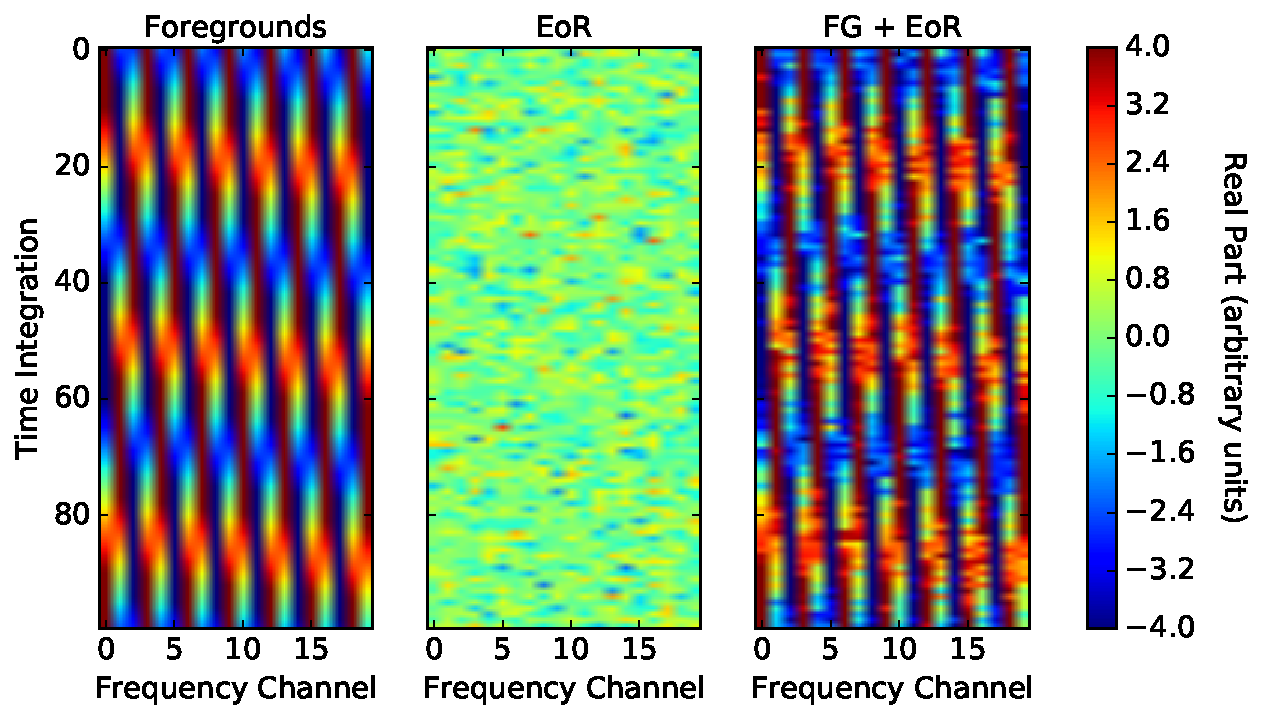
\includegraphics[trim={0cm 0cm 0cm 0cm},clip,width=\columnwidth]{plots/toy_sigloss1.pdf}
	\caption{Our toy model dataset to which we apply different weighting schemes to in order to investigate signal loss. We model a mock foreground-only visibility with a sinusoid signal that varies smoothly in 
time and frequency. We model a mock visibility of an EoR signal as a random Gaussian signal. We add the two together to form $\textbf{x} = 
\textbf{x}_{\rm FG} + \textbf{x}_{\rm EoR}$. Real parts are shown here.}
	\label{fig:toy_sigloss1}
\end{figure}

%First, 
We compute the power spectrum of our toy model dataset $\textbf{x}$ using Equations \eqref{eq:qhat} and \eqref{eq:phat}, with $\textbf{R} \equiv \widehat{\textbf{C}}^{-1}$.  Figure \ref{fig:toy_sigloss12} shows the estimated covariances of our toy model datasets along with the $\widehat{\textbf{C}}^{-1}$ weighted data. The foreground sinusoid is clearly visible in $\widehat{\textbf{C}}_{\rm FG}$.  The power spectrum result is shown in green in the left plot of Figure \ref{fig:toy_sigloss3}. Also plotted in the figure are the uniform-weighted ($\textbf{R} \equiv \textbf{I}$) power spectrum of the individual components $\textbf{x}_{\rm FG}$ (blue) and $\textbf{x}_{\rm EoR}$ (red). As shown, our $\widehat{\textbf{C}}^{-1}$ weighted result successfully suppresses foregrounds,
%For our toy model, the successful suppression of the foreground mode is 
demonstrated in Figure \ref{fig:toy_sigloss3} by the missing foreground peak in the weighted power spectrum estimate (green).  It is also evident that our result fails to recover the EoR signal --- it exhibits the correct shape, but the amplitude level is slightly low.  It is this behavior which we describe as signal loss.

\begin{figure}
	\centering
	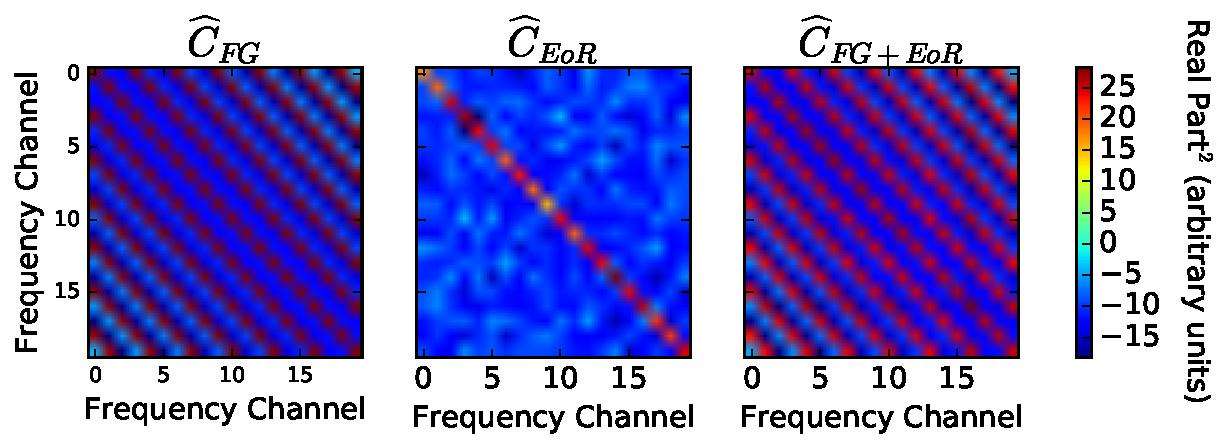
\includegraphics[trim={0cm 0cm 0cm 0cm},clip,width=\columnwidth]{plots/toy_sigloss12.pdf}
	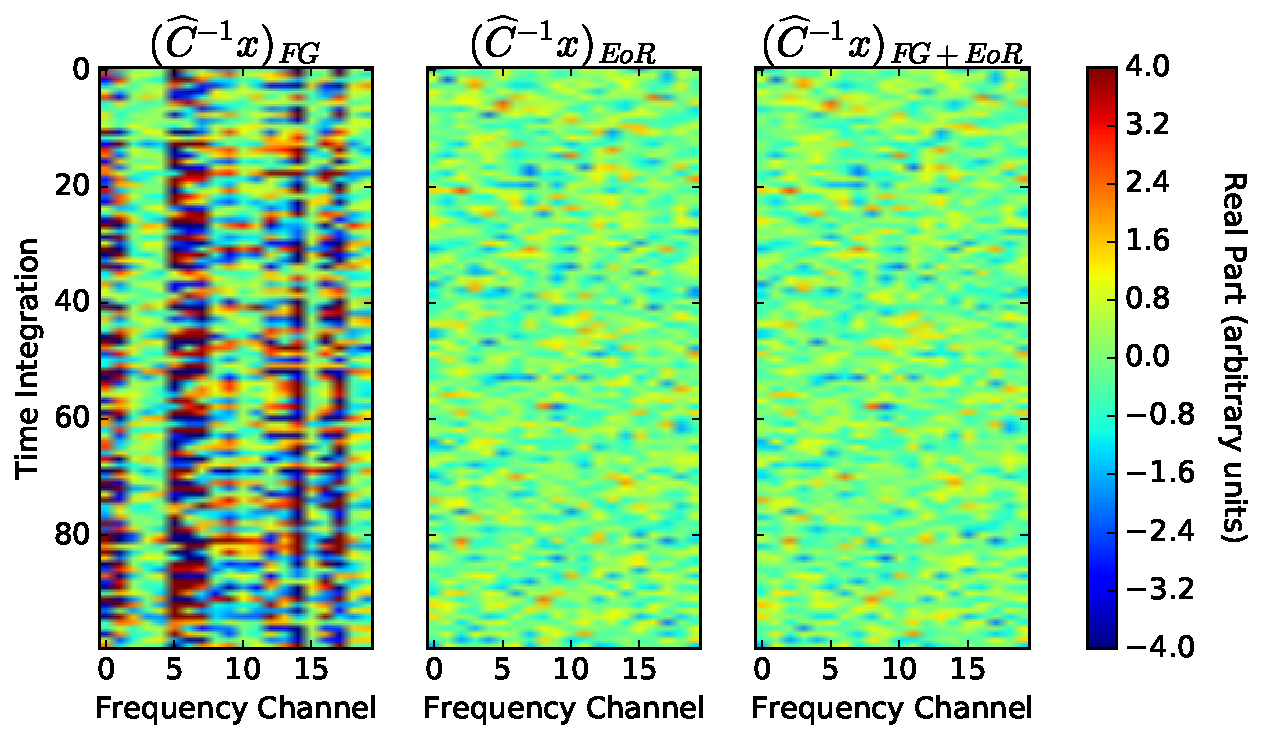
\includegraphics[trim={0cm 0cm 0cm 0cm},clip,width=\columnwidth]{plots/toy_sigloss13.pdf}
	\caption{The estimated covariance matrices (top row) and inverse covariance-weighted data (bottom row) for FG only (left), EoR only 
(middle), and FG + EoR (right). Real parts are shown here.}
	\label{fig:toy_sigloss12}
\end{figure}

\begin{figure*}
	\centering
	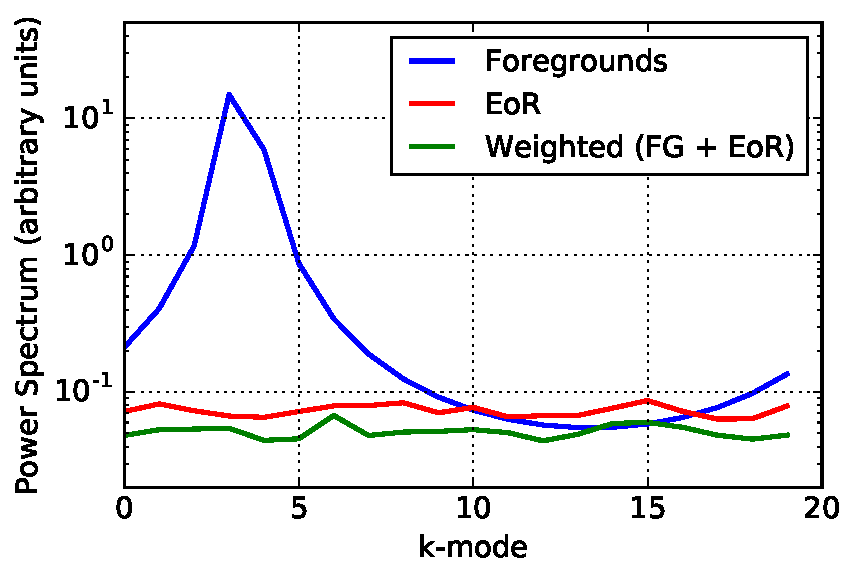
\includegraphics[trim={0cm 0cm 0cm 0cm},clip,height=0.33\textwidth]{plots/toy_sigloss3.pdf}
	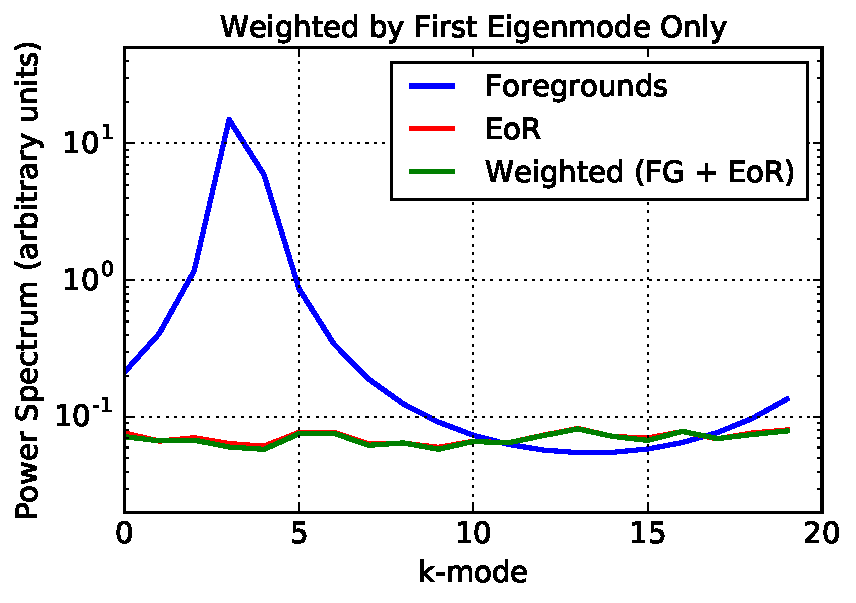
\includegraphics[trim={0cm 0cm 0cm 0cm},clip,height=0.33\textwidth]{plots/toy_sigloss4.pdf}
	\caption{Resulting power spectrum estimates for the toy model simulation described in Section \ref{sec:toymodel} --- foregrounds only (blue), EoR only (red), and the weighted FG + EoR dataset (green). The power spectrum of the foregrounds peaks at a $k$-mode based on the frequency of the sinusoid used to create the mock FG signal. In the two panels, we compare using empirically estimated inverse covariance weighting where $\textbf{C}$ is derived from the data (left), and projecting out the zeroth eigenmode only (right). In the former case, signal loss arises from the coupling of the eigenmodes of $\widehat{\textbf{C}}$ to the data. 
% JEA - redundant
%For an empirically estimated $\widehat{\textbf{C}}$, 
%its eigenvalues differ from those of the true covariance, where 
%the coupling between EoR-dominated eigenmodes and the data can lead to loss.
%Hence, 
There is negligible signal loss when all eigenmodes besides the foreground one are no longer correlated with the data.
%assigning identical weights to all eigenmodes except the first, 
%constructing a covariance proportional to the identity and the outer product of the sinusoid eigenmode, since we are only down-weighting the FG-dominated mode in this case.
}
	\label{fig:toy_sigloss3}
\end{figure*}

As discussed in Section \ref{sec:QE}, this behavior is {\it not} expected in the case that we were to use a true $\textbf{C}^{-1}$ weighting.  Rather, we would obtain %the behavior shown in the toy model in Appendix \ref{sec:icw_appendix}\footnote{Note that there the true covariance matrix is also the sum of a diagonal portion describing the signal, and a single mode describing the contaminant (similar to Figure \ref{fig:toy_sigloss12}).}, with suppression of the foreground mode resulting in 
a nearly unbiased estimate of the power spectrum.   The key difference is that since $\widehat{\textbf{C}}$ is estimated from the data, its eigenvectors and eigenvalues are strongly coupled to the particular data realization that was used to compute it, and this coupling leads to loss.

For the case of an eigenmode which can be safely assumed to be predominantly a foreground, its presence in the true covariance matrix will result in the desired suppression via a kind of projection; whether or not it is strongly correlated with the the actual data vector is irrelevant.  However, in the case of an empirically estimated covariance matrix, the eigenmodes of $\widehat{\textbf{C}}_{\rm EoR}$ will both be incorrect and can be correlated with the data. If these incorrect eigenmodes are not correlated with the data, it will lead to non-minimum variance estimates but will not produce the suppression of the power spectrum amplitude as seen in the left plot of Figure \ref{fig:toy_sigloss3}. As described in Section \ref{sec:siglossmethod}, however, if $\widehat{\mathbf{C}}_{\rm EoR}$ $\textit{is}$ correlated with the data vector $\mathbf{x}$, there is a kind of projection of power in the {\it non}-foreground modes from the resulting power spectrum estimate, thus producing an estimate that is biased low.  In short, {\it if the covariance is computed from the data itself, it carries the risk of overfitting information in the data and introducing a multiplicative bias (per $k$) to estimates of the signal.} 

%For a toy model mathematical derivation of signal loss arising from a data-estimated covariance matrix, see Appendix \ref{sec:sigloss_appendix}. Here we will describe the origin of this signal loss intuitively.

%% JEA - I don't think the eigenspectrum really helps, but at some point we probably want to show it ...
%To begin to understand the lossy behavior of this result, we can closely study our estimated covariance eigenspectrum, shown in Figure \ref{fig:toy_sigloss2}. Since it is estimated from our data, its eigenspectrum differs from the eigenspectrum of the true covariance $\textbf{C}$, and this difference has important consequences on our result. 
%
%An eigenspectrum ranks the eigenvalues of a matrix from highest to lowest and can be thought of as a spectrum of weights that are given to each spectral mode in the data. In other words, the eigenvalues encode the strength of different shapes in the dataset. The eigenspectrum of the identity matrix $\textbf{I}$ is flat (all $1$'s) because it gives equal weighting to all modes. In our application, covariance matrices tend to have sloped eigenspectra, meaning that modes are given different weights in QE power spectrum estimation. 
%% JEA - I think this is actually NOT true - see the toy model as an example.  The size of the eigenvalues isn't what determines that the undesired mode is downweighted and the others left alone.  I haven't computed the eigenvalues explicitly, but down-weighting of m occurs regardless of the relative size of s and u.
%The modes with the highest eigenvalues are down-weighted the most. 

%\begin{figure}
%	\centering
%	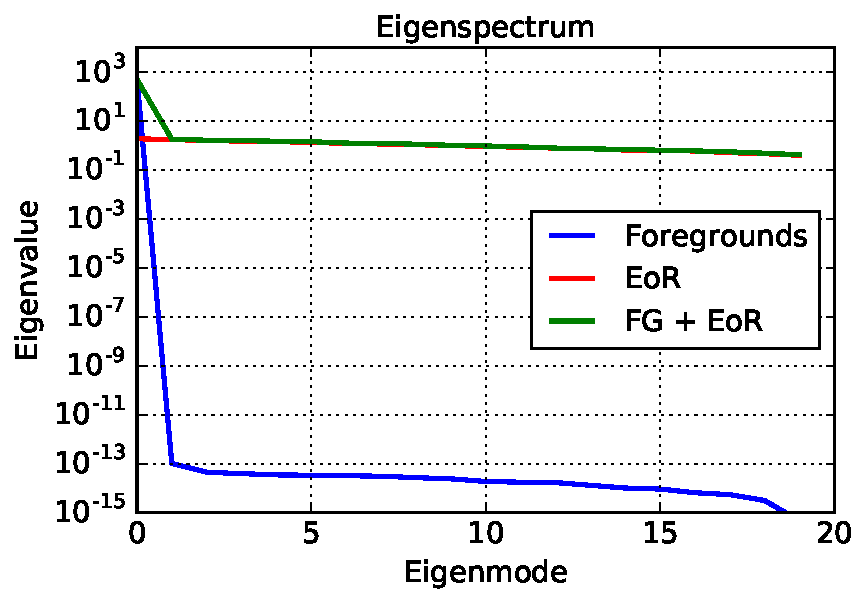
\includegraphics[trim={0cm 0cm 0cm 0cm},clip,width=\columnwidth]{plots/toy_sigloss2.pdf}
%	\caption{Eigenspectrum of $\widehat{\textbf{C}}_{\rm FG}$ (blue), $\widehat{\textbf{C}}_{\rm EoR}$ (red), and $\widehat{\textbf{C}}_{\rm FG+EoR}$ 
%(green). The eigenspectrum of $\widehat{\textbf{C}}_{\rm FG}$ peaks at the zeroth eigenmode, due to the presence of only one sinusoid. These empirically estimated covariance matrices have eigenspectra that are different from that of the true $\textbf{C}$. Specifically, these eigenmodes have the risk of being down-weighted more significantly than they should be because they are coupled to the data in a way that produces loss.}
%	\label{fig:toy_sigloss2}
%\end{figure}

%We show the {\it eigenspectrum} (the eigenvalues of the matrix in descending order) of this toy model in Figure \ref{fig:toy_sigloss2}.  In this case,
%For example, 
%the largest-valued eigenmode of $\widehat{\textbf{C}}$ (highest eigenvalue) describes the sinusoid foreground mode in the toy model (the peak in Figure \ref{fig:toy_sigloss3}). 
% 


%In general, the highest-valued eigenmodes of $\widehat{\textbf{C}}$ typically (but not always) describe bright foregrounds --- the most prominent shapes in a dataset. For these FG-dominated modes, where foregrounds outshine the EoR signal, down-weighting is beneficial. In some sense, we desire signal loss in this regime, if by `signal' we mean `foregrounds.' In this case it is beneficial for these eigenmodes to be coupled to the data in a way that produces loss. 



%If the true covariance matrix $\textbf{C}$ of our data was known, then every single eigenvalue and eigenvector of $\textbf{C}$ would be 
%representative of real fluctuations in the data. However, when using an estimated $\widehat{\textbf{C}}$ that is derived from one 
%particular data realization, its eigenvalues and eigenvectors may differ from the truth. Said differently, shapes that may not exist (or exist rarely) in a true covariance may appear stronger in the estimated covariance. Hence, they will be down-weighted 
%more than they should be.



The danger of an empirically estimated covariance matrix comes mostly from not being able to describe the EoR-dominated eigenmodes of $\textbf{C}$ accurately, for which the EoR signal is brighter than foregrounds. In such a case, the coupling between these modes to the data realization leads to the overfitting and subtraction of the EoR signal. More specifically, the coupling between the estimated covariance and the data is anti-correlated in nature (which is explained in more detail in Section \ref{sec:siglossmethod}), which leads to loss. Mis-estimating $\textbf{C}$ for EoR-dominated eigenmodes is therefore more harmful than for FG-dominated modes, and since the lowest-valued eigenmodes of an eigenspectrum are typically EoR-dominated, using this part of the spectrum for weighting is most dangerous.

Armed with this information,
%Using what we've learned about the eigenspectrum, 
we can tweak the covariance in a simple way to suppress foregrounds and yield minimal signal loss. Recall that our toy model foreground 
% JEA - modes need not be sinusoids; the point is that there is one outer product describing this in the covariance
%is a sinusoid, so it 
can be perfectly described by a single eigenmode. Using the full dataset's (foreground plus EoR signal) empirical covariance, we can 
project out the zeroth eigenmode and 
%then flatten the rest of the spectrum to have eigenvalues of 1, thereby down-weighting the foreground-dominated mode more than the rest of the modes. Hence, we are changing the EoR-dominating part of the spectrum to be less coupled to the data, limiting the amount of overfitting that can happen for those modes (i.e., only allowing overfitting to occur for the first mode).
then take the remaining covariance to be the identity matrix.  
This decouples the covariance from the data for the EoR modes.  The resulting power spectrum estimate for this case is shown in the right plot of Figure \ref{fig:toy_sigloss3}. 
In this case we recover the EoR signal, demonstrating that if we can disentangle the foreground-dominated modes and EoR-dominated modes, we can suppress
% down-weight them 
foregrounds with negligible signal loss. 

Altering $\widehat{\textbf{C}}$ as such is one specific example of a regularization method for this toy model, in which we are changing $\widehat{\textbf{C}}$ in a way that reduces its coupling to the data realization. There are several other simple ways to regularize $\widehat{\textbf{C}}$, and we will discuss some in Section 
\ref{sec:otherweight}.

\subsection{Fringe-Rate Filtering}
\label{sec:toymodel_frf}

We have shown how signal loss can arise due to the coupling of EoR-dominated eigenmodes to the data. We will next show how this effect is exacerbated by reducing the total number of independent samples in a dataset. 

A fringe-rate filter is an analysis technique designed to maximize sensitivity by integrating in time (\citealt{parsons_et_al2016}). Rather than a traditional box-car average in time, a time domain filter can be designed to up-weight temporal modes consistent with the sidereal motion on the sky, while down-weighting modes that are noise-like. 

Because fringe-rate filtering is analogous to averaging in time, it comes at the cost of reducing the total number of independent samples in the data. With fewer independent modes, it becomes more difficult for the empirical covariance to estimate the true covariance matrix of the fringe-rate filtered data. We can quantify this effect by evaluating a convergence metric $\varepsilon(\Chat)$ for the empirical covariance, which we define as

% JEA - Death to eigenspectra!
%The resulting eigenspectrum as compared to the green curve (FG + EoR) in Figure \ref{fig:toy_sigloss2} is shown in Figure \ref{fig:toy_sigloss15}. 

\begin{equation}
\label{eq:converge}
\varepsilon (\Chat) \equiv \sqrt{\frac{\sum_{ij} (\widehat{C}_{ij} - {C}_{ij})^2}{\sum_{ij} {C}_{ij}^2}},
\end{equation}
where $\C$ is the true covariance matrix. To compute this metric, we draw different numbers of realizations (different draws of Gaussian noise) of our toy model EoR measurement, $\textbf{x}_{\rm EoR}$, and take their ensemble average. We then compare this to the ``true" covariance, which in our simulation is set to be the empirical covariance after a large number ($500$) of realizations. As shown in Figure \ref{fig:toy_sigloss16}, we perform this computation for a range of total independent ensemble realizations (horizontal axis) and number of independent samples in the data following time-averaging, or ``fringe-rate filtering" (different colors). With more independent time samples (i.e., more realizations) in the data, one converges to the true fringe-rate filtered covariance more quickly. 

The situation here with using a finite number of time samples to estimate our covariance is analogous to a problem faced in galaxy surveys, where the non-linear covariance 
of the matter power spectrum is estimated using a large --- but finite --- number of expensive simulations. There, the limited 
number of independent simulations results in inaccuracies in estimated covariance matrices 
\citep{dodelson_schneider2013,taylor_joachimi_etal2014}, which in turn result in biases in the final parameter constraints 
\citep{hartlap_et_al2007}. In our case, the empirically estimated covariances are used for estimating the power spectrum, and 
as we discussed in the previous section (and will argue more thoroughly in Section \ref{sec:siglossmethod}), couplings between these covariances and the data can lead to power spectrum estimates that are biased 
\emph{low}---which is precisely signal loss. In future work, it will be fruitful to investigate whether advanced techniques from the 
galaxy survey literature for estimating accurate covariance matrices can be successfully adapted for $21\,\textrm{cm}$ 
cosmology. These techniques include the imposition of sparsity priors \citep{padmanabhan_et_al2016}, the fitting of 
theoretically motivated parametric forms \citep{pearson_samushia2016}, covariance tapering \citep{paz_sanchez2015}, 
marginalization over the true covariance \citep{sellentin_heavens2016}, and shrinkage methods 
\citep{pope_szapudi2008,joachimi_2017}.

%Just as important as the eigenvalues are the eigenvectors of our empirical covariances. 
The overall convergence of the covariance is important, but also noteworthy is the fact that different eigenvectors converge to their true forms at different rates. This is illustrated by Figure \ref{fig:toy_sigloss17}, which shows the convergence of eigenvectors in an empirical estimate of a covariance matrix. For this particular toy model, we construct a covariance whose true form combines the same mock foreground from the previous toy models with an EoR component that is modeled as a diagonal matrix with eigenvalues spanning one order of magnitude (more specifically, we construct the EoR covariance as a diagonal matrix in the Fourier domain, where the signal is expected to be uncorrelated; its Fourier transform is then the true covariance of the EoR in the frequency domain, or $\textbf{C}_{\rm EoR}$). For different numbers of realizations, we draw random EoR signals that are consistent with $\textbf{C}_{\rm EoR}$, add them to the mock foreground data, and compute the combined empirical covariance by averaging over the realizations. The eigenvectors of this empirical covariance are then compared to the true eigenvectors $\widehat{\textbf{v}}$, where we use as a convergence metric $\varepsilon(\widehat{\textbf{v}})$, defined as:
\begin{equation}
\label{eq:converge_eig}
\varepsilon (\widehat{\textbf{v}}) \equiv \sqrt{\sum_{i}^{N_{f}}|\textbf{v}-\widehat{\textbf{v}}|_{i}^2},
\end{equation}
where $N_{f}$ is the number of frequencies ($20$) in the mock data. The eigenmode convergence curves in Figure \ref{fig:toy_sigloss17} are ranked ordered by eigenvalue, such that ``Eigenmode \#0" illustrates the convergence of the eigenvector with the largest eigenvalue, ``Eigenmode \#1" for the second largest eigenvalue, and so on. We see that the zeroth eigenmode --- the mode describing the foreground signal --- is quickest to converge.

Our numerical test reveals that the convergence rates of empirical eigenvectors is related to the sample variance in our empirical estimate. In general, computing an empirical covariance from a finite ensemble average means that the empirical eigenmodes have sample variances. Consider first a limiting case where all eigenvalues are equal. In such a scenario, any linear combination of eigenvectors is also an eigenvector, and thus there is no sensible way to define the convergence of eigenvectors. In our current test, aside from the zeroth mode, the eigenvalues have similar values but are not precisely equal. Hence, there is a well-defined set of eigenvectors to converge to. However, due to the sample variance of our empirical covariance estimate, there may be accidental degeneracies between modes, where some modes are mixing and swapping with others. Therefore, the steeper an eigenspectrum, the easier it is for the eigenmodes to decouple from each other and approach their true forms. A particularly drastic example of this can be seen in the behavior of mode $0$ (the foreground mode), whose eigenvalue differs enough from the others that it is able to converge reasonably quickly despite substantial sample variance in our empirical covariance estimate. To break degeneracies in the remaining modes, however, requires many more realizations.

While the connection between the rate of convergence of an empirical eigenvector with the sample variance of an eigenspectrum is interesting, it is also important to note that regardless of convergence rate, any mode that is coupled to the data is susceptible to signal loss. The true eigenvectors are not correlated with the data realizations; thus, if our empirical eigenvectors are converged fully, there will not be any signal loss. However, an unconverged eigenvector estimate will retain some memory of the data realizations used in its generation, leading to signal loss.

In the toy models throughout Section \ref{sec:SiglossOverview}, we exploit the fact that the strongest eigenmode (highest eigenvalue mode) is dominated by foregrounds in order to purposely incur signal loss for that mode. Even for the case of real PAPER data (Section \ref{sec:CaseStudy}), we make the assumption that the strongest eigenmodes are likely the most contaminated by foregrounds. However, in general, foregrounds need not be restricted to the strongest eigenmodes, and as we have seen, it is really the degeneracies between modes that determines how quickly they converge, and hence how much signal loss can result.

%One sees that the highest-valued eigenmodes converge to their true eigenvectors more quickly. With only a small number of realizations, these empirically estimated modes already retain little correlation with the specific realizations of data that were used to form the empirical covariance. As we will see in the next section, using only these eigenmodes, which are less coupled to data realizations, minimizes signal loss. In contrast, the lower-valued eigenmodes retain more memory of the data realizations, which leads to correlations that induce signal loss. 
% JEA - this is redundant
%Said differently, a steep covariance eigenspectrum can be especially dangerous because the eigenmodes that converge the slowest are typically also EoR-dominated and are therefore susceptible to the most loss.  %\acl{Think about whether we need to do the Fourier space version as well.}

% JEA - death to eigenspectra!
%\begin{figure}
%	\centering
%	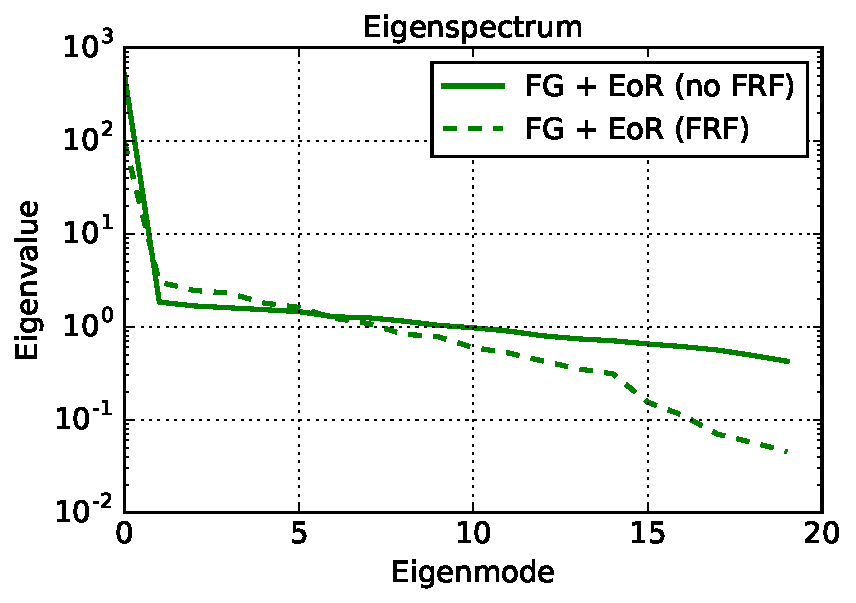
\includegraphics[trim={0cm 0cm 0cm 0cm},clip,height=0.31\textwidth]{plots/toy_sigloss15.pdf}
%	\caption{Eigenspectrum of $\widehat{\textbf{C}}_{\rm FG+EoR}$, in the case of no fringe-rate filtering (solid green) and with fringe-rate filtering (dashed green). The dashed, steep eigenspectrum has a greater risk of signal loss because its lowest-valued eigenmodes are both more strongly coupled to the data (than those of the solid eigenspectrum) and, in this example, are also EoR-dominated.}
%	\label{fig:toy_sigloss15}
%\end{figure}

\begin{figure}
	\centering
	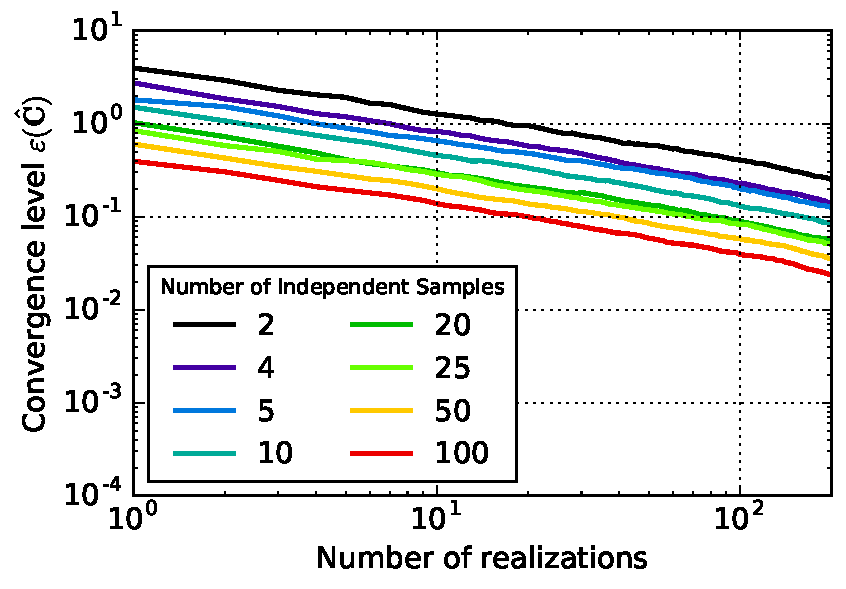
\includegraphics[width=\columnwidth]{plots/toy_sigloss16.pdf}
	\caption{The convergence level, as defined by Equation \eqref{eq:converge}, of empirically estimated covariances of mock EoR signals with different numbers of independent samples. In red, the mock EoR signal is comprised entirely of independent samples (100 of them). Subsequent colors show time-averaged signals. As the number of realizations increases, we see that the empirical covariances approach the true covariances. With more independent samples, the quicker an empirical covariance converges (i.e., the quicker it decouples from the data), and the less signal loss we would expect to result.}
	\label{fig:toy_sigloss16}
\end{figure}

\begin{figure}
	\centering
	\includegraphics[width=\columnwidth]{plots/toy_sigloss17.pdf}
	\caption{The convergence level, as defined by Equation \eqref{eq:converge_eig}, of empirically estimated eigenvectors for different numbers of mock data realizations. The colors span from the 0th eigenmode (has the highest eigenvalue) to the 19th eigenmode (has the lowest eigenvalue), where they are ordered by eigenvalue in descending order. This figure shows that the zeroth eigenmode converges the quickest, implying that eigenvectors with eigenvalues that are substantially different than the rest (the FG-dominated mode has a much higher eigenvalue than the EoR modes) are able to converge to the true eigenvectors the quickest. On the other hand, eigenmodes $1$-$19$ have similar eigenvalues and are slower to converge because of degeneracies between them.}
	\label{fig:toy_sigloss17}
\end{figure}

\begin{figure}
	\centering
	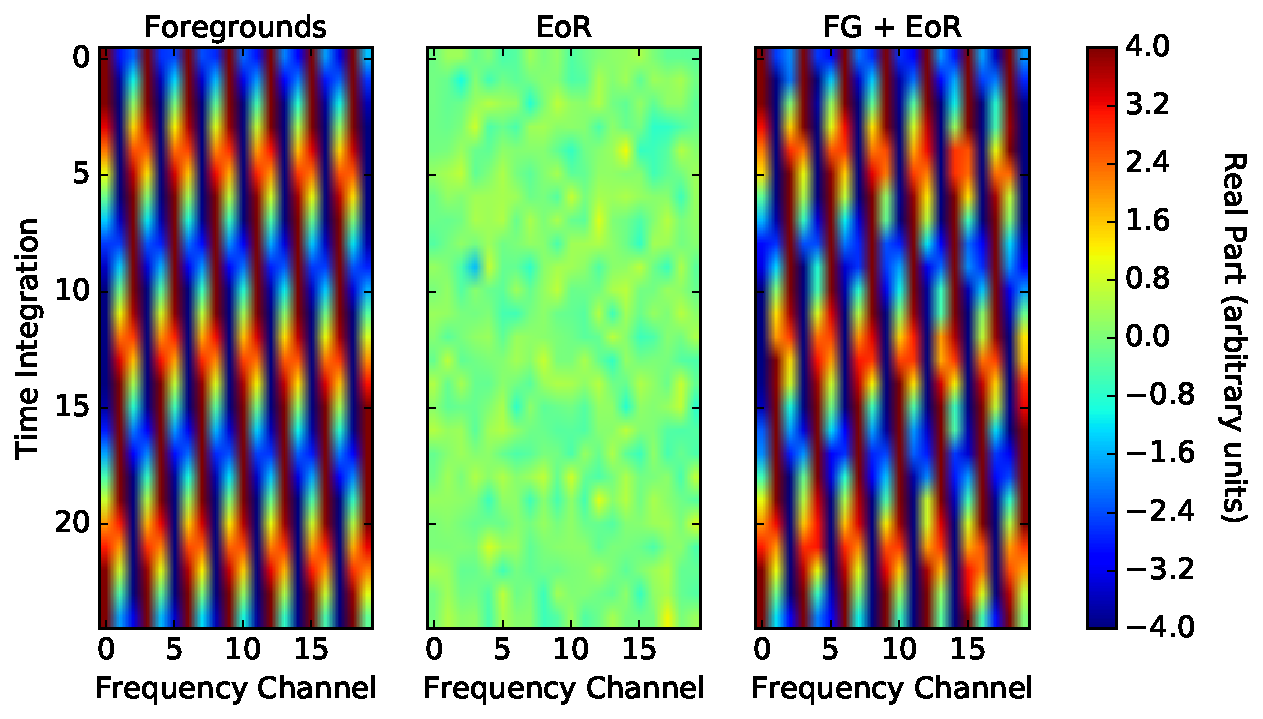
\includegraphics[width=\columnwidth]{plots/toy_sigloss5.pdf}
	\caption{Our ``fringe-rate filtered" (time-averaged) toy model dataset. We average every four samples together, 
yielding $25$ independent samples in time. Real parts are shown here.}
	\label{fig:toy_sigloss5}
\end{figure}

\begin{figure}
	\centering
	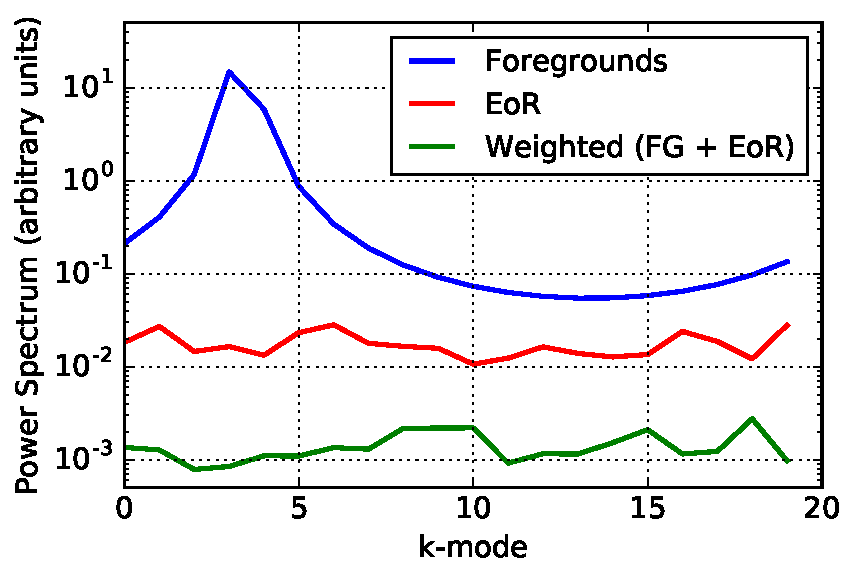
\includegraphics[trim={0cm 0cm 0cm 0cm},clip,width=\columnwidth]{plots/toy_sigloss7.pdf}
	\caption{Resulting power spectrum estimate for the ``fringe-rate filtered" (time-averaged) toy model simulation --- foregrounds only (blue), 
EoR only (red), and the weighted FG + EoR dataset (green). We use empirically estimated inverse covariance weighting where $\textbf{C}$ is 
computed from the data. There is a larger amount of signal loss than for the non-averaged data, a consequence of weighting by eigenmodes that are more strongly coupled to the data due to there being fewer independent modes in the data.}
	\label{fig:toy_sigloss7}
\end{figure}


With Figures \ref{fig:toy_sigloss16} and \ref{fig:toy_sigloss17} establishing the connection between convergence rates (of empirical covariances and eigenvectors) and number of realizations, we now turn back to our original toy model used in Section \ref{sec:toymodel}, which is comprised of a mock foreground and mock EoR signal. We mimic a fringe-rate filter by averaging every four time integrations of our toy model dataset together, yielding $25$ independent samples in time (Figure \ref{fig:toy_sigloss5}). We choose these numbers so that the total number of independent samples is similar to the number of frequency channels --- hence our matrices will be full rank. We use this ``fringe-rate filtered" mock data for the remainder of Section \ref{sec:SiglossOverview}.
%\footnote{If instead we average every $20$ samples together, yielding only $5$ independent samples in time, we are left with a rank deficient covariance matrix. In this case... \cc{fill in}}

The power spectrum results for this model are shown in Figure \ref{fig:toy_sigloss7}, and as 
expected there is a much larger amount of signal loss for this time-averaged dataset since we do a worse job estimating the true covariance. In addition, as a result of having fewer independent samples, we obtain an estimate with more scatter. This is evident by noticing that the 
green curve in Figure \ref{fig:toy_sigloss7} fails to trace the shape of the uniform-weighted EoR power spectrum (red). %It is worth noting that a hybrid method, where the empirical covariance is calculated using the original dataset (not fringe-rate filtered) but applied to the filtered dataset, results in less loss than what is exhibited in Figure \ref{fig:toy_sigloss7} (though still lossy). This approach is worth exploring in future work; however in this paper we focus solely on ways to calculate and minimize loss associated with weighting a dataset based on itself (rather than weights associated with a dataset produced by a separate analysis).

Using our toy model, we have seen that a sensitivity-driven analysis technique like fringe-rate filtering has trade-offs of signal 
loss and noisier estimates when using data-estimated covariance matrices. Longer integrations increase sensitivity but reduce 
the number of independent samples, resulting in 
eigenmodes correlated with the data
% JEA - it's not that they are wrong, but that they are correlated
%poorly characterized, steep eigenspectra 
that can overfit signal greatly. We 
note that a fringe-rate filter does have a range of benefits, many described in \citet{parsons_et_al2016}, so it can still be 
advantageous to use one despite the trade-offs.

\subsection{Other Weighting Options}
\label{sec:otherweight}

In Section \ref{sec:toymodel} we showed one example of how altering $\widehat{\textbf{C}}$ can 
make the difference between nearly zero and some signal loss. We will now use our toy model to describe several other ways to tailor $\widehat{\textbf{C}}$ 
in order to minimize signal loss. We choose four independent regularization methods to highlight in this section, which have 
been chosen due to their simplicity in implementation and straightforward interpretations. We illustrate the resulting power 
spectra for the different cases in Figure \ref{fig:toy_sigloss8}.
% and \ref{fig:toy_sigloss14}. 
These examples are not meant to be taken as suggested analysis methods but rather as illustrative cases. 

As a first test, we model the covariance matrix of EoR as a proof of concept that if perfect models are known, signal loss can be 
avoided. We know that our simulated EoR signal should have a covariance matrix that mimics the identity matrix, with its 
variance encoded along the diagonal. We model $\textbf{C}_{\rm EoR}$ as such (i.e., the identity), instead of computing it based on $\textbf{x}
_{\rm EoR}$ itself. Next, we add $\textbf{C}_{\rm EoR} + \widehat{\textbf{C}}_{\rm FG}$ (where $\widehat{\textbf{C}}_{\rm FG} = \langle\textbf{x}_{\rm FG}
\textbf{x}_{\rm FG}^{\dagger}\rangle_{t}$) to obtain a final $\widehat{\textbf{C}}_{\rm reg}$ (regularized empirical covariance matrix) to use in weighting. In Figure \ref{fig:toy_sigloss8} (upper 
left), we see that there is negligible signal loss. This is because by modeling $\textbf{C}_{\rm EoR}$, we avoid overfitting EoR fluctuations in the data that our model doesn't know about (but, an empirically derived $\widehat{\textbf{C}}_{\rm EoR}$ would know about the fluctuations). 
%This is also shown by comparing the (steeper) green and (flatter) red curves in Figure \ref{fig:toy_sigloss14}. 
In practice such a weighting option is not feasible, as it is difficult to model $\textbf{C}_{\rm EoR}$, and $\widehat{\textbf{C}}_{\rm FG}$ is unknown because we do not know how to separate out the foregrounds from the EoR in our data.

\begin{figure*}
	\centering
	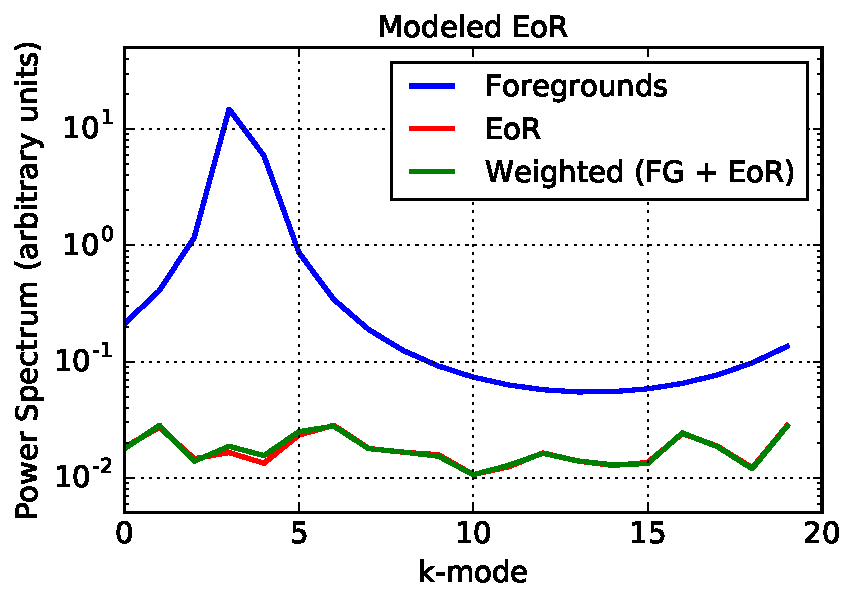
\includegraphics[trim={0cm 0cm 0cm 0cm},clip,height=0.3\textwidth]{plots/toy_sigloss10.pdf}
	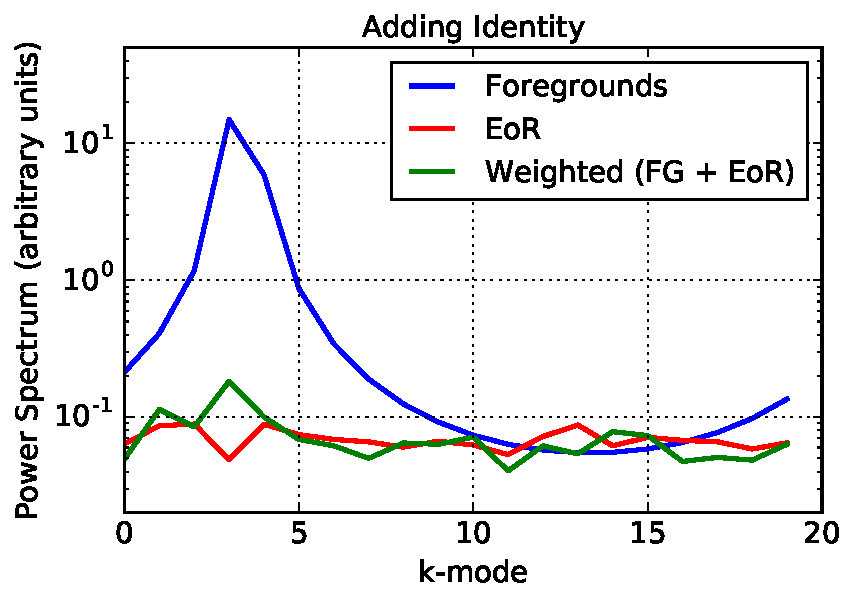
\includegraphics[trim={0cm 0cm 0cm 0cm},clip,height=0.3\textwidth]{plots/toy_sigloss8.pdf}
	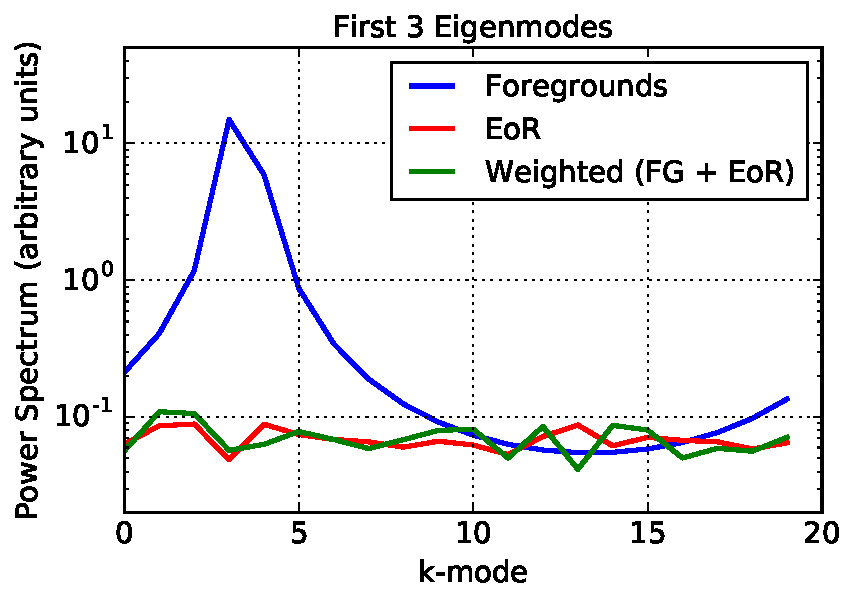
\includegraphics[trim={0cm 0cm 0cm 0cm},clip,height=0.3\textwidth]{plots/toy_sigloss9.pdf}
	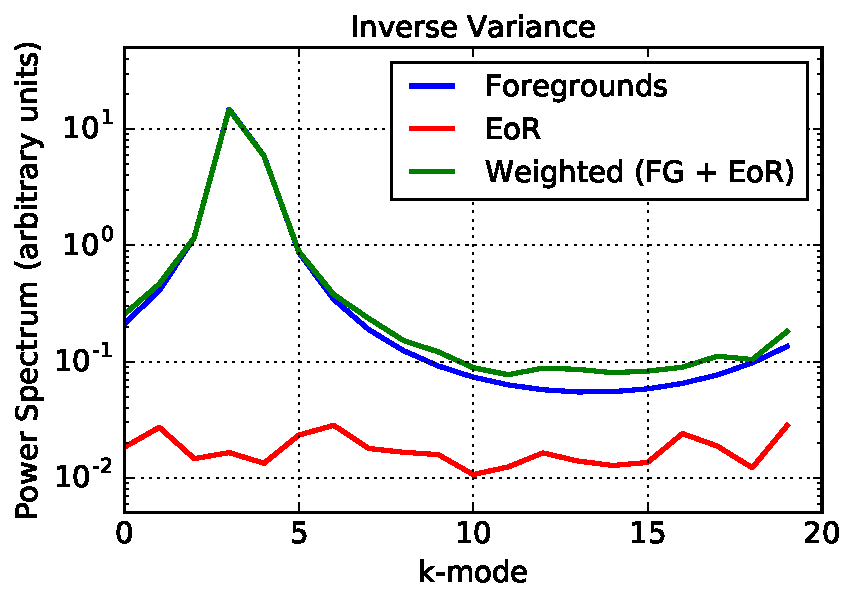
\includegraphics[trim={0cm 0cm 0cm 0cm},clip,height=0.3\textwidth]{plots/toy_sigloss11.pdf}
	\caption{Resulting power spectra estimates for our ``fringe-rate filtered" (time-averaged) toy model simulation --- foregrounds only (blue), EoR only (red), and the weighted FG + EoR dataset (green). We show four alternate weighting options that each minimize signal loss, including modeling the covariance matrix of EoR (upper left), regularizing $\widehat{\textbf{C}}$ by adding an identity matrix to it (upper right), using only the first three eigenmodes of $\widehat{\textbf{C}}$ (lower left), and keeping only the diagonal elements of $\widehat{\textbf{C}}$ (lower right). The first case (upper left) is not feasible in practice since we do not know $\textbf{C}_{\rm FG}$ and $\textbf{C}_{\rm EoR}$ like we do in the toy model.}
	\label{fig:toy_sigloss8}
\end{figure*}

%\begin{figure}
%	\centering
%	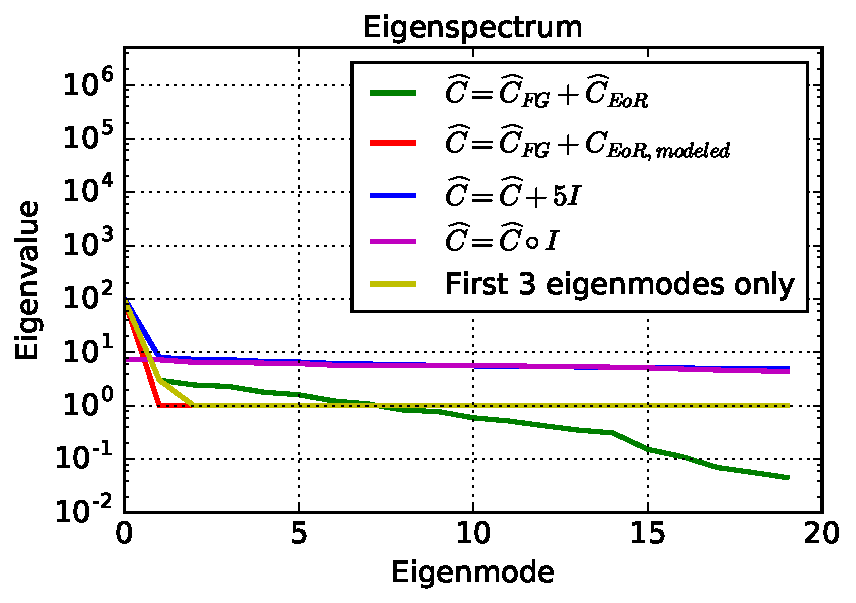
\includegraphics[trim={0cm 0cm 0cm 0cm},clip,width=\columnwidth]{plots/toy_sigloss14.pdf}
%	\caption{We compare the eigenspectrum of an empirically calculated $\widehat{\textbf{C}}$ (green) to that of four alternate 
%weighting options, including modeling the covariance matrix of EoR (red), regularizing $\widehat{\textbf{C}}$ by adding an identity 
%matrix to it (blue), using only the first three eigenmodes of $\widehat{\textbf{C}}$ (yellow), and multiplying an identity matrix with $
%\widehat{\textbf{C}}$ (magenta). All eigenspectra (except the green) are relatively flat and don't exhibit signal loss. All were 
%computed for the `fringe-rate filtered' (time-averaged) toy model case presented in Section \ref{sec:toymodel_frf}.}
%	\label{fig:toy_sigloss14}
%\end{figure}
%
The second panel (top right) in Figure \ref{fig:toy_sigloss8} uses a regularization method of setting $\widehat{\textbf{C}}_{\rm reg} \equiv 
\widehat{\textbf{C}} + \gamma\textbf{I}$, where $\gamma = 5$ (an arbitrary strength 
of $\textbf{I}$ for the purpose of this toy model). By adding the identity matrix, element-wise, we are weighting the diagonal 
elements of the estimated covariance matrix more heavily than those off-diagonal. Since the identity component does not know anything about the data realization, it alters the covariance to be less coupled to the data and there is no loss. %Although there is negligible signal loss using this regularization, the small green peak at the fourth $k$-mode represents residual foregrounds that still exist since the shapes encoded in the off-diagonal frequency correlations of the covariance matrix were deemed not as prominent as the diagonal elements using this weighting scheme. 

The third panel (bottom left) in Figure \ref{fig:toy_sigloss8} minimizes signal loss by only using the first three eigenmodes of the estimated covariance. Recalling that our toy model foregrounds can be described entirely by the zeroth eigenmode, this 
method intentionally projects out the highest-valued modes only by replacing all but the three highest weights in the 
eigenspectrum with $1$'s (equal weights). Again, avoiding the overfitting of EoR-dominated modes which are coupled to the data results in negligible signal loss. While this case is illuminating for the toy model, in practice it is not obvious which eigenmodes are foreground or EoR dominated (and they could be mixed as well), so determining which subset of modes to down-weight is not trivial. We experiment with this idea using PAPER data in Section \ref{sec:Weight}.

The last regularization scheme we are highlighting here is setting $\widehat{\textbf{C}}_{\rm reg} \equiv \widehat{\textbf{C}} \circ \textbf{I}$ (element-wise multiplication), or inverse variance weighting (i.e., keeping only the diagonal elements of $\widehat{\textbf{C}}$). In the bottom right 
panel of Figure \ref{fig:toy_sigloss8}, we see that this method does not down-weight the foregrounds at all --- this regularization altered $\widehat{\textbf{C}}$ in a way where it is no longer coupled to \textit{any} of the empirically estimated eigenmodes, including the FG-dominated one. To understand this, we recall that our foregrounds are spread out in frequency and therefore have non-negligible frequency-frequency correlations. Multiplying by 
the identity matrix, element-wise, results in a diagonal matrix, meaning we do not have any correlation information. Because of this, we do a poor job 
suppressing the foreground. But because we decoupled the whole eigenspectrum from the data, we also avoid signal loss. Although this method did not successfully recover the EoR signal for this particular simulation, it is important that we show that there 
are many options for estimating a covariance matrix, and some may down-weight certain eigenmodes more effectively than others based on the spectral nature 
of the components in a dataset. 
%One may imagine a situation where a particular systematic is contained to an isolated 
%frequency (such as radio frequency interference or crosstalk). In such a case, preserving only the diagonal elements of $
%\widehat{\textbf{C}}$ would be an effective way of removing this contamination. 

In summary, we have shown how signal loss is caused by weighting a dataset by itself, and in particular how estimated covariances can overfit EoR modes when they are coupled to data and not converged to their true forms. We have also seen that there are trade-offs between a chosen weighting method, its foreground-removal effectiveness, the number of independent samples in a dataset, and the amount of resulting signal loss. 


% SECTION 3 CASE STUDY ---------------------------------------------------------------------------------

\section{Signal Loss in PAPER-64}
\label{sec:CaseStudy}

We now turn to a detailed signal loss investigation using a subset of the PAPER-64 dataset from \citetalias{ali_et_al2015}. In the previous section we showed how signal loss arises when weighting data with empirically estimated covariances; in this section we highlight how the amount of this loss was underestimated in the previous analysis. Additionally, we illustrate how we have revised our analysis pipeline in light of our growing understandings.

As a brief review, PAPER is a dedicated 21\,cm experiment located in the Karoo Desert in South Africa. The PAPER-64 
configuration consists of 64 dual-polarization drift-scan elements that are arranged in a grid layout. For our case study, we 
focus solely on Stokes I estimated data \citep{moore_et_al2013} from PAPER's $30$ m East/West baselines (Figure 
\ref{fig:ant_layout}). All data is compressed, calibrated (using self-calibration and redundant calibration), delay-filtered (to remove foregrounds inside the wedge), LST-binned, and fringe-rate filtered. For detailed information about the backend system of PAPER-64, its observations, and data reduction pipeline, we 
refer the reader to \citet{parsons_et_al2010} and \citetalias{ali_et_al2015}. We note that all data processing steps are identical to those in \citetalias{ali_et_al2015} until after the LST-binning step in Figure 3 of \citetalias{ali_et_al2015}.

\begin{figure}
	\centering
	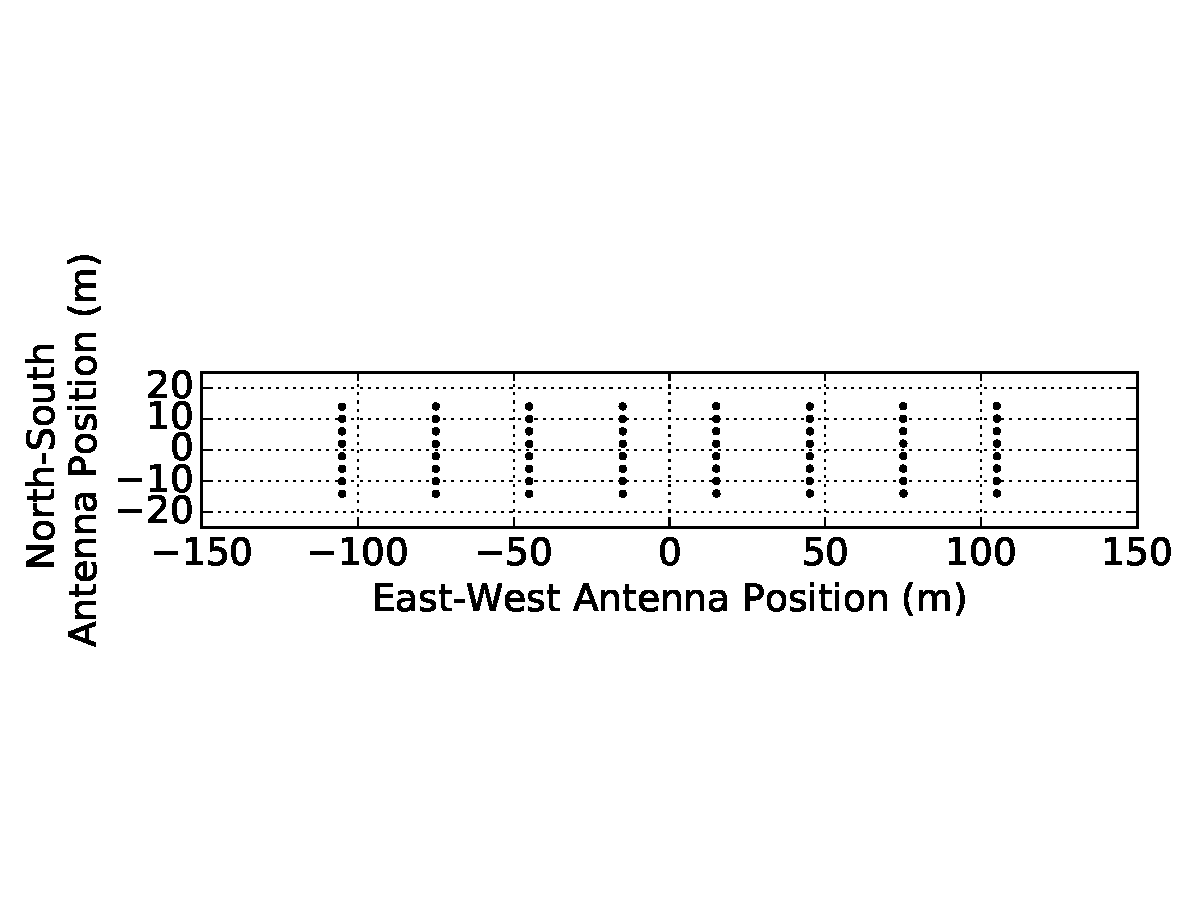
\includegraphics[trim={0cm 0cm 0cm 0cm},width=\columnwidth]{plots/ant_layout_aspect.pdf}
	\caption{The PAPER-64 antenna layout. We use only $10$ of the $30$ m East/West baselines for the analysis in this 
paper (i.e., a subset of the shortest horizontal spacings).}
	\label{fig:ant_layout}
\end{figure}

The previously best published 21\,cm upper limit result from \citetalias{ali_et_al2015} placed a $2\sigma$ upper limit 
on $\Delta^{2}(k)$, defined as

\begin{equation}
\Delta^{\textbf{2}}(k) = \frac{k^{3}}{2\pi^{2}}\,\hat{P}(k),
\end{equation}

\noindent of $(22.4$ mK$)^{2}$ in the range $0.15 < k < 0.5$\,$h$ Mpc$^{-1}$ at $z = 8.4$. The need to revise this limit stems mostly from previously underestimated signal loss, which we 
address in this section.

For the analysis in this paper, we use $8.1$ hours of LST, namely an RA range of $0.5$-$8.6$ hours (\citetalias{ali_et_al2015} uses a slightly longer RA 
range of $0$-$8.6$ hours; we found that some early LSTs were more severely foreground contaminated). We also use only $10$ baselines, a subset of the $51$ total East/West baselines used in \citetalias{ali_et_al2015}, in order to illustrate our revised methods. All power spectrum results are produced for a center frequency of 151\,MHz using a width of 10\,MHz ($20$ channels), identical to the analysis in \citetalias{ali_et_al2015}. In the case study in this paper, we only use one baseline type instead of the three as in 
\citetalias{ali_et_al2015}, but Kolopanis et al. (\textit{in prep.}) uses the full dataset presented in \citetalias{ali_et_al2015} to revise the result and place limits on the EoR at multiple redshifts (using a straightforward and not lossy approach to avoid many of the issues that will be made clear later on).

The most significant changes from \citetalias{ali_et_al2015} occur in our revised power spectrum analysis, which is explained in the rest of this paper, but we also note that the applied fringe-rate filter is also slightly different. In \citetalias{ali_et_al2015}, the 
applied filter was not equivalent to the optimal fringe-rate filter (which is designed to maximize power spectrum sensitivity). Instead, the optimal filter was degraded slightly by widening it in fringe-rate space. This was chosen in order to increase the number of independent 
modes and reduce signal loss associated with the quadratic estimator, though as we will explain in the next section, this signal loss was still underestimated. With the development of a new, 
robust method for assessing signal loss, we choose to use the optimal filter in order to maximize sensitivity. This filter is 
computed for a fiducial 30\,m baseline at 150\,MHz, the center frequency in our band. The filter in both the fringe-rate 
domain and time domain is shown in Figure \ref{fig:frp}.

Finally, we emphasize that the discussion that follows is solely focused on signal loss associated with empirical covariance weighting. As mentioned in Section \ref{sec:SiglossOverview}, there are a number of steps in our analysis pipeline which could lead to loss, including gain calibration, delay filtering, and fringe-rate filtering, which have been investigated at various levels of detail in \citet{parsons_et_al2014} and \citetalias{ali_et_al2015} but are clearly the subject of future work. Here we only focus on the most significant source of loss we have identified and note that Kolopanis et al. (\textit{in prep.}) and other future work will consider additional sources of signal loss and exercise increased caution in reporting results.

\begin{figure}
	\centering
	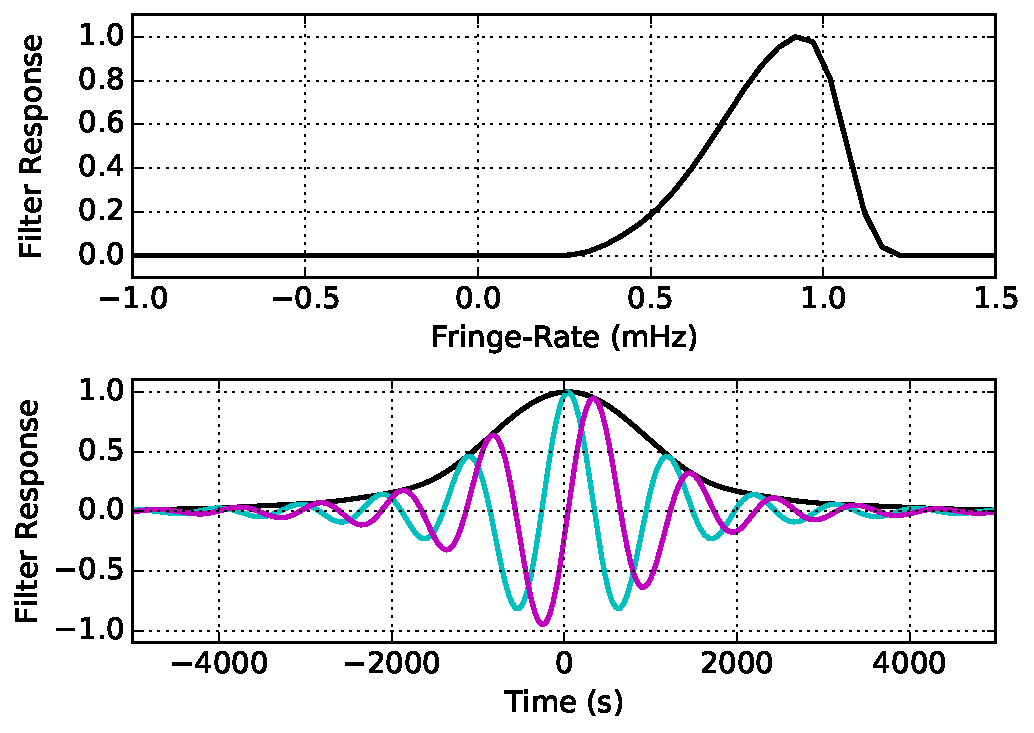
\includegraphics[width=\columnwidth]{plots/frp.pdf}
	\caption{Top: the normalized optimal power-spectrum sensitivity weighting in fringe-rate space for our fiducial baseline and 
Stokes I polarization beam. Bottom: the time domain convolution kernel corresponding to the top panel. Real and imaginary 
components are illustrated in cyan and magenta, respectively, with the absolute amplitude in black. The fringe-rate filter acts as 
an integration in time, increasing sensitivity but reducing the number of independent samples in the dataset.}
	\label{fig:frp}
\end{figure}

We present our PAPER-64 signal loss investigation in three parts. We first give an overview of our signal injection framework which is used to estimate loss. In this framework (and as in \citetalias{ali_et_al2015}), we inject simulated cosmological signals into our data and test the recovery of those signals (an approach also taken by \citet{masui_et_al2013}). As we will see, correlations between the injected signals and the data are significant complicating factors which were previously not taken into account. Next, we describe our methodology in practice and detail how we map our simulations into a posterior for the EoR signal. Finally, we build off of the previous section by experimenting with different regularization schemes on PAPER data in order to minimize loss. Throughout each section, we also highlight major differences from the signal loss computation used in \citetalias{ali_et_al2015}.


% SECTION 3 SIGNAL LOSS ---------------------------------------------------------------------------------

\subsection{Signal Loss Methodology} 
\label{sec:siglossmethod}
In short, our method for estimating signal loss consists of adding an EoR-like signal into visibility data and then measuring how much of this injected signal would be detectable given any attenuation of this signal by the (lossy) data analysis pipeline.  To capture the full statistical likelihood of signal loss, one requires a quick way to generate many realizations of simulated 21\,cm signal visibilities. Here we use the same method as in \citetalias{ali_et_al2015}, where mock Gaussian noise visibilities (mock EoR signals) 
are filtered in time using an optimal fringe-rate filter to retain only ``sky-like" modes. Since the optimal filter has a shape that matches the rate of the sidereal motion of the sky, this transforms the Gaussian noise into a measurement that PAPER could make. This signal is then added to the visibility data.\footnote{One 
specific change from \citetalias{ali_et_al2015} is that we add this simulated signal - which has been fringe-rate filtered once already in order to transform it into a ``sky-like" signal - into the analysis pipeline before a fringe-rate filter is 
applied to the data (i.e., prior to the analysis step of fringe-rate filtering). Previously, the addition was done after the fringe-rate filter analysis step.  This change results in an increased 
estimate of signal loss, %(by a factor of $\sim$$10$), 
likely due to the use of the fringe-rate filter as a simulator. However, this pipeline difference, while significant, is not the dominant reason why signal loss was underestimated in \citetalias{ali_et_al2015} (the dominant reason is explained in the main text in Section \ref{sec:siglossmethod}).}

Mathematically, suppose that $\textbf{e}$ is the mock injected EoR signal (at some amplitude level). We do not know the true EoR signal contained within our visibility data, $\textbf{x}$, so $\textbf{e}$ takes on the role of the true EoR signal (for which we measure its loss). Furthermore, one can make the assumption that the true EoR signal is small within our measured data, so the data vector $\textbf{x}$ itself is representative of mostly contaminants. Using this assumption, the sum of $\textbf{x}$ and $\textbf{e}$, defined as $\textbf{r}$:

\begin{equation}
\label{eq:rxe}
\textbf{r} = \textbf{x} + \textbf{e},
\end{equation}
can be thought of as the sum of contaminants plus EoR. The quantity $\textbf{r}$ then becomes the dataset for which we are measuring how much loss of $\textbf{e}$ there is due to our power spectrum pipeline.

We are interested in quantifying how much variance in $\textbf{e}$ is lost after weighting $\textbf{r}$ and estimating the power 
spectrum according to QE formalism. We investigate this by comparing two quantities we call the input power spectrum and 
output power spectrum: $\widehat{P}_{\rm in}$ and $\widehat{P}_{\rm out}$, estimated using QE as

\begin{equation}
\label{eq:Pin}
\widehat{P}_{\rm in}^{\alpha} \equiv \text{M}^{\alpha}_{\rm in}\textbf{e}^{\dagger}\textbf{I}\textbf{Q}^{\alpha}\textbf{I}\textbf{e}
\end{equation}

\noindent and

\begin{eqnarray}
\label{eq:sigloss}
\widehat{P}_{\rm out}^{\alpha} &\equiv& \widehat{\textbf{P}}_{r}^{\alpha} \nonumber\\%-\widehat{\textbf{P}}_{x,\alpha} \nonumber \\
&=& \text{M}^{\alpha}_{r}\textbf{r}^{\dagger}\textbf{R}_{r}\textbf{Q}^{\alpha}\textbf{R}_{r}\textbf{r},% - \text{M}^{\alpha}_{x}\textbf{x}^{\dagger}\textbf{R}_{x}\textbf{Q}^{\alpha}\textbf{R}_{x}\textbf{x},
\end{eqnarray}
where, for illustrative purposes and notational simplicity, we have written these equations with scalar normalizations M, even though for our numerical results we choose a diagonal matrix normalization using $\mathbf{M}$ as in Equation \eqref{eq:phat}.

The quantity $\widehat{P}_{\rm in}$, defined by Equation \eqref{eq:Pin}, is a uniformly weighted estimator of the power spectrum of $\mathbf{e}$. It can be considered the power spectrum of this particular realization of the EoR; alternatively, it can be viewed as the true power spectrum of the injected signal up to cosmic variance fluctuations. The role of $\widehat{P}_{\rm in}$ in our analysis is to serve as a reference for the power spectrum that would be measured if there were no signal loss or other systematics. The input power spectrum is then to be compared to $\widehat{P}_{\rm out}$, which approximates the (lossy) power spectrum estimate that is output by our analysis pipeline prior to any signal loss adjustments. 

%In the limit where no significant cross-correlations between the data and the injected signals are found, this will recover the amount of injected power spectrum remaining after the covariance weighting operation (i.e., the amount of background EoR power, $P_{\rm eor}$, not removed by the foreground down-weighting procedure). In other words, we make the anzatz that 

%\begin{equation}
%\widehat{P}_{\rm out} = \widehat{\textbf{P}}_{x} \label{eqn:anzatz},
%\end{equation}
%and folding in our definition from Equation \eqref{eq:sigloss}, this ansatz implies that we are seeking the injected 
%signal amplitude which causes a power doubling ($\phat_r = 2 \phat_x$). \cc{I am unsure of this power doubling thing} 

Under this injection framework, we can begin to see explicitly why there can be large signal loss. Expanding out Equation \eqref{eq:sigloss}, $\widehat{P}_{\rm out}$ becomes:

%
%In short, we can approximate a signal loss estimate as the ratio of $\widehat{P}_{\rm out}/P_{\rm in}$, evaluated at the data level $\widehat{\textbf{P}}_{x}$. We motivate the fact that we can evaluate the output-to-input power spectrum ratio at $\widehat{\textbf{P}}_{x}$ by the following reasoning (and then detail our signal loss estimation in practice in the sections that follow).
%
%In the limit of no instrumental noise, the data that we measure, $\x$, is comprised of two signals, such that
%\begin{equation}
%\x \equiv \f + \s,
%\end{equation}
%where $\mathbf{f}$ represents the foregrounds and $\mathbf{s}$ represents the cosmological signal. In general, suppose that our power spectrum algorithm passes the data through some function $g$, yielding a lossy estimate of the power spectrum $\phat_{x}$. This can be parametrized as
%\begin{equation}
%\label{eq:LinearPspecSum}
%\langle \phat_{x} \rangle  = \langle g(\x) \rangle = \ell_{\rm fg} \p_{\rm fg} + \ell_{\rm eor} \p_{\rm eor},
%\end{equation}
%where $\ell_{\rm eor}$ and $\ell_{\rm fg}$ are multiplicative factors accounting for the signal loss in the true EoR 
%power spectrum $\p_{\rm eor}$ and true foreground power spectrum $\p_{\rm fg}$, respectively. It is not 
%\emph{a priori} obvious why this parameterization is suitable; we thus provide a toy model in Appendix 
%\ref{sec:sigloss_appendix} to motivate this, although it should be noted that the derivation is an approximation 
%which assumes that the covariance used in the QE analysis is close to the true covariance with effects due to 
%small sample size limited to first order perturbations and thus neglects cross-correlation between $x$ and $e$.  
%In actual fact the sample size is similar to the number of independent modes, a case were one expects cross 
%terms to be remain significant.   
%
%Given this form, a suitable estimate for $\p_{\rm eor}$ would be $\phat_{x} / \ell_{\rm eor}$, or the uncorrected power spectrum of data divided by the signal loss estimate. Although such an estimate leaves an additive bias from foregrounds (see Section \ref{sec:BiasTypes}) that must be mitigated by other methods (as is the case for any attempt to measure the $21\,\textrm{cm}$ power spectrum), it normalizes $\p_{\rm eor}$ back to its correct level such that there is no multiplicative bias. The most conceptually straightforward way to compute $\ell_{\rm eor}$ is to model the foregrounds and EoR signal via simulations, and then to form the quantity
%\begin{equation}
%\label{eq:Deriv1}
%\widehat{\ell}_{\rm eor} = \frac{g(\f + \s) - g(\f)}{\p_{\rm eor}}.
%\end{equation}
%However, this approach assumes that we have sufficiently good knowledge of our foreground and signal models, which is certainly not the case --- if it were, it would be simpler to construct our covariance matrices from our models, avoiding signal loss altogether! Instead, we can use the data itself as our model of the foregrounds, injecting a new EoR signal $\e$ (with power spectrum $P_{in}$), computing instead
%\begin{equation}
%\label{eq:Deriv2}
%\widehat{\ell}_{\rm eor} = \frac{g(\x+ \e) - g(\x)}{P_{in}},
%\end{equation}
%which reduces to the same result because of the linearity of Equation \eqref{eq:LinearPspecSum}. Essentially, one is computing the slope of $\langle \phat_{x} \rangle$ with respect to $\p_{\rm eor}$ (note that both Equations \eqref{eq:Deriv1} and \eqref{eq:Deriv2} take the form of finite difference derivatives). Under the approximation that the relation between the two quantities is linear, it does not matter whether this slope is evaluated about $\x$ or $\f$. In reality, one expects some deviations from linearity, but Equation \eqref{eq:Deriv2} remains a good approximation of Equation \eqref{eq:Deriv1} as long as $\x$ is dominated by $\f$. 
%
%Using this motivation, the numerator of Equation \eqref{eq:Deriv2} is precisely our expression for $\widehat{P}_{\rm out}$ (Equation \eqref{eq:sigloss}), and the denominator is $P_{\rm in}$ (Equation \eqref{eq:Pin}), where the function $g$ is our QE power spectrum pipeline. \dcj{Here is the post-hoc justification for this signal loss method.  Except goes back to assumption of equation for g which just \emph{assumes} that there are no cross-terms in the estimation of a power spectrum. So we're just kicking the can down the road.} \acl{Ok, in my defense, Equation \eqref{eq:LinearPspecSum} is a little better than an \emph{assumption}. Appendix \eqref{sec:sigloss_appendix} does in fact illustrate this with an example. The crucial question is whether we're allowed to motivate our method based on a relationship that is only true in expectation. Note that this expectation includes allowances for signal loss due to the cross-correlation between signal and foregrounds, with an example of this being Appendix \ref{sec:sigloss_appendix}.}
%\jp{I'm fine with leaving the text as is and calling this note closed with the addition of the appendix, but will wait for sign off from DCJ.}
%\dcj{ Assuming that expansion to "leading order in $\eta$" means $\eta<<1$ then the approximation is that the 
%covariance is nearly perfectly calculated from the data with only small effects due to finite samples. Thus 
%correlations don't make it into the expression and foregrounds remain uncorrelated with eor or injected signals.  
%I added words explaining this but it still looks strange for us to be saying that loss is linear in one section and 
%then explaining in the next section exactly how cross-terms were what messed us up in the first go round.} 
%\acl{Ok, I'm open to suggestions as to how to phrase this, because lots of people seem to be thinking that the appendix was meant to justify everything. It's not. It's meant as a motivational example. I just wanted something where I could follow through analytically to the end to show that it's ok to think about signal loss as a multiplicative factor. At least in expectation. And then how one deals with not correcting for the signal loss in expectation is described in Section \ref{sec:Practice}.}
%
%Effectively, this means that the relationship between the input and output power spectra, $P_{\rm in}$ and $\widehat{P}_{\rm out}$, can be thought of as a transfer function 
%which, for a sampling of $P_{\rm in}$ and $\widehat{P}_{\rm out}$ provides a mapping from an input power spectrum distribution into an output 
%distribution. By viewing data through this signal loss lens, we may then ask the question ``what input power spectrum 
%distribution could this (signal-loss affected) data come from?" 
%
%In Section \ref{sec:Illustration}, we provide some intuition for how the transfer function is able to capture signal loss. Section \ref{sec:Practice} then details the numerical computations used to translate our power spectrum result into one viewed through a 
%signal loss lens. We note that interpretation of the signal injection results can be framed in multiple ways which yield similar but not identical answers. One alternative to the method described in Section \ref{sec:Practice} is described in Appendix \ref{sec:Pr_appendix}.
%%We showcase two methods... \cc{fill in with some broad statement of why we're showing 2 methods but also state that they yield similar results...}

%\subsubsection{Signal Loss Illustration}
%\label{sec:Illustration}
%To explore how our expression for $\widehat{P}_{\rm out}$ encapsulates signal loss, we expand out Equation \eqref{eq:sigloss}:

\begin{eqnarray}
\label{eq:crossterm_full}
\widehat{P}_{\rm out}^{\alpha} &=& \text{M}^{\alpha}_{r}(\textbf{x}+\textbf{e})^{\dagger}\textbf{R}_{r}\textbf{Q}^{\alpha}\textbf{R}_{r}(\textbf{x}+\textbf{e}) \nonumber \\%- 
%\text{M}^{\alpha}_{x}\textbf{x}^{\dagger}\textbf{R}_{x}\textbf{Q}^{\alpha}\textbf{R}_{x}\textbf{x} \nonumber \\
&=& \text{M}^{\alpha}_{a}\textbf{x}^{\dagger}\textbf{R}_{r}\textbf{Q}^{\alpha}\textbf{R}_{r}\textbf{x} + \text{M}^{\alpha}_{b}\textbf{e}^{\dagger}\textbf{R}_{r}\textbf{Q}
^{\alpha}\textbf{R}_{r}\textbf{e} \nonumber \\
&+& \text{M}^{\alpha}_{c}\textbf{x}^{\dagger}\textbf{R}_{r}\textbf{Q}^{\alpha}\textbf{R}_{r}\textbf{e} + \text{M}^{\alpha}_{d}\textbf{e}^{\dagger}\textbf{R}_{r}\textbf{Q}^{\alpha}\textbf{R}_{r}\textbf{x}. %\nonumber \\
%&-& \text{M}^{\alpha}_{x}\textbf{x}^{\dagger}\textbf{R}_{x}\textbf{Q}^{\alpha}\textbf{R}_{x}\textbf{x}.
\end{eqnarray}
Assuming \textbf{R}$_{r}$ is symmetric, the two cross-terms (terms with one copy of $\textbf{e}$ and one copy of $\textbf{x}$) can be summed together as:

\begin{eqnarray}
\label{eq:crossterm}
\widehat{P}_{\rm out}^{\alpha} &= &  \text{M}^{\alpha}_{a}\textbf{x}^{\dagger}\textbf{R}_{r}\textbf{Q}^{\alpha}\textbf{R}_{r}\textbf{x} + \text{M}^{\alpha}_{b}\textbf{e}^{\dagger}\textbf{R}_{r}\textbf{Q}
^{\alpha}\textbf{R}_{r}\textbf{e} \nonumber \\
&+& 2 \text{M}^{\alpha}_{c}\textbf{x}^{\dagger}\textbf{R}_{r}\textbf{Q}^{\alpha}\textbf{R}_{r}\textbf{e}. %\nonumber \\
%&-& \text{M}^{\alpha}_{x}\textbf{x}^{\dagger}\textbf{R}_{x}\textbf{Q}^{\alpha}\textbf{R}_{x}\textbf{x}.
\end{eqnarray}
One of the key takeaways of this section is that the \citetalias{ali_et_al2015} analysis estimated signal loss by comparing \textit{only} the signal-only term (second term in Equation \eqref{eq:crossterm}) with $\widehat{P}_{\rm in}$, whereas in fact the cross-term (third term in Equation \eqref{eq:crossterm}) can substantially lower $\widehat{P}_{\rm out}$. In order to investigate the effect of each of these terms on signal loss, all three components are plotted in Figure \ref{fig:sigloss_terms} for two cases: empirically estimated inverse covariance weighting ($\textbf{R}_{r} \equiv \widehat{\textbf{C}}_{r}^{-1}$) and uniform weighting ($\textbf{R}_{r} \equiv \textbf{I}$). We will now go into further detail and examine the behavior of this equation in three different regimes of the injected signal - very weak (left ends of the $P_{\rm in}$ axes in Figure \ref{fig:sigloss_terms}), very strong (right ends), and in between (middle portions).

{\bf Small injection:}
%In this regime, the first term in Equation \eqref{eq:crossterm} is very similar to the power spectrum of data alone, namely $\text{M}^{\alpha}_{a}\textbf{x}^{\dagger}\textbf{R}_{r}\textbf{Q}^{\alpha}\textbf{R}_{r}\textbf{x} \sim \text{M}^{\alpha}_{x}\textbf{x}^{\dagger}\textbf{R}_{x}\textbf{Q}^{\alpha}\textbf{R}_{x}\textbf{x}$. They differ only in their covariance matrices, and when the injected signal is very small compared to the data, their difference can be neglected. 
%This is shown by the black and gray curves converging in both panels of Figure \ref{fig:sigloss_terms}. 
In this regime, the cross-terms (red) behave as noise averaged over a finite number of samples. Output values are Gaussian distributed around zero, spanning a range of values set by the injection level. This is because $\widehat{\textbf{R}}_{r}$ is dominated by the data $\textbf{x}$, avoiding correlations with $\textbf{e}$ that can lead to solely negative power (explained further below). In fact, for the uniformly weighted case, the cross-term  $\text{M}^{\alpha}_{x}\textbf{x}^{\dagger}\textbf{I}\textbf{Q}^{\alpha}\textbf{I}\textbf{e}$ is well modeled as a symmetric distribution with zero mean and width $\sqrt{\widehat{\textbf{P}}_e}\sqrt{\widehat{\textbf{P}}_x}$. We also note that in this regime, $\widehat{\textbf{P}}_{r}$ (black) approaches the data-only power spectrum value (gray) as expected. %In this limit we might imagine that the cross-correlation should also be small, enabling us to recover just the EoR term. However, examining the cross-term plotted in Figure \ref{fig:sigloss_terms} (red) in the identity case (right plot), we see that this term is still large enough to have a significant impact on $\widehat{P}_{\rm out}$. It is in this regime where we're dominated by biases from the cross-terms, causing the difference between the signal-only term (green) and $\widehat{P}_{\rm out}$ (black). We also note that the cross-terms behave as noise at small injections even in the inverse covariance weighted case (left plot), spanning a range of values set by the injection level. This is because $\widehat{\textbf{C}}_{r}$ is dominated by the data $\textbf{x}$, avoiding correlations with $\textbf{e}$ that can lead to solely negative power (explained further below).

{\bf Large injection:}
When the injected signal is much larger than the measured power spectrum, the data-only components can 
be neglected as they are many orders of magnitude smaller. We include a description of this regime for completeness in our discussion, but note that the upper limits that we compute are typically not determined by simulations in this regime (i.e., in using an empirical weighting scheme we've assumed the data to be dominated by foregrounds rather than the cosmological signal).  However, it is useful as a check of our system in a relatively simple case. As we can see from Figure \ref{fig:sigloss_terms}, the cross-terms (red) are small in comparison to the signal-only term (green). Here only does the signal-only term used in \citetalias{ali_et_al2015} dominate the total power output. We again see that, in the empirical inverse covariance weighted case, the cross-terms behave as noise (positive and negative fluctuations around zero mean). This is for the same reason as at small injections --- here $\widehat{\textbf{C}}_{r}$ is dominated by the signal $\textbf{e}$. The cross-correlation can again be modeled as a symmetric distribution of zero mean and width $\sqrt{\widehat{\textbf{P}}_e}\sqrt{\widehat{\textbf{P}}_x}$.

{\bf In between:}
When the injected signal is of a similar amplitude to the data by itself, the situation becomes less straightforward. We see that 
the weighted injected power spectrum component mirrors the input power indicating little loss (i.e., the green curve follows the dotted black line), eventually 
departing from unity when the injected amplitude is well above the level of the data power spectrum. However, 
in this regime the cross-term (red) has nearly the same amplitude, but with a negative sign. As explained below, this negativity is the result of cross-correlating inverse covariance weighted terms.  This negative component drives down the $\widehat{P}_{\rm out}$ estimator (black). Again, we emphasize that in \citetalias{ali_et_al2015}, signal loss was computed by only looking at the second term in Equation \eqref{eq:crossterm} (green), which incorrectly implies no loss at the data-only power spectrum level. Ignoring the effect of the negative power from the cross-terms is the main reason for underestimating power spectrum limits in \citetalias{ali_et_al2015}.

%A brief description of Figure \ref{fig:sigloss_terms} is as follows. The gray curve represents the data level, which is constant as the level of $P_{\rm in}$, the input EoR signal, is changed. The blue curve is the power spectrum of the data only, weighted by an empirical covariance estimated from the data plus the EoR signal ($\widehat{\textbf{C}}_{r}^{-1}$). It approaches the gray at low injection level, as expected, since in that case $\widehat{\textbf{C}}_{r}^{-1} \rightarrow \widehat{\textbf{C}}_{x}^{-1}$. The green curve is the power spectrum of the EoR signal, weighted by $\widehat{\textbf{C}}_{r}^{-1}$. This is the exact term that was compared to $P_{\rm in}$ in the \citetalias{ali_et_al2015} signal loss analysis, and in doing so this would imply there is negligible loss (where the green crosses the gray). It is primarily due to the cross-terms (red), that the black curve exhibits $\sim$$3$ orders of magnitude of loss at the data level, for the inverse covariance weighted case. We see that the cross-terms can produce a large, negative signal which serves to reduce $\widehat{P}_{\rm out}$ and drive the bulk of our loss. In the unweighted case, however (right plot), the cross-terms primarily drive a tail of `excess' $\widehat{P}_{\rm out}$ at low injects, though at larger injects we see unity transfer as expected (the solid black curve lies on the dotted black line, which represents unity transfer).

%\dcj{This section isn't held up by figure 17. Is that because the "illustriative" figure is off? Or is it that cross-terms don't matter when injected signal is very large.}
%We now turn to building intuition behind the negative power that arises from the cross-terms in Equation \eqref{eq:crossterm}. For illustrative purposes in this subsection only, we consider a scenario where $\textbf{e}$ dominates compared to $\textbf{x}$. It is in this limit where we expect signal loss to be greatest, and $\widehat{P}_{\rm out}$ becomes:
%
%\begin{eqnarray}
%\label{eq:pout_expand}
%P_{\rm out, \alpha} &\approx&  M^{\alpha}_{b}\textbf{e}^{\dagger}\textbf{R}_{r}\textbf{Q}^{\alpha}\textbf{R}_{r}\textbf{e} +
% 2M^{\alpha}_{c}\textbf{x}^{\dagger}\textbf{R}_{r}\textbf{Q}^{\alpha}\textbf{R}_{r}\textbf{e}.
%\end{eqnarray}
%The first term of $\widehat{P}_{\rm out}$ is simply the weighted power spectrum of $\textbf{e}$ alone. Again, it is this quantity that was used in \citetalias{ali_et_al2015} to calculate signal loss. However, without taking into account the cross-terms (the second term), we can substantially underestimate loss. In short, this is because correlations between the data and injected EoR signal emerge as statistical noise that is added to the power spectrum estimate, decreasing the value of $\widehat{P}_{\rm out}$. Including these cross-terms in our new analysis represents the bulk change of our revised analysis compared to \citetalias{ali_et_al2015}.

\begin{figure*}
	\centering
	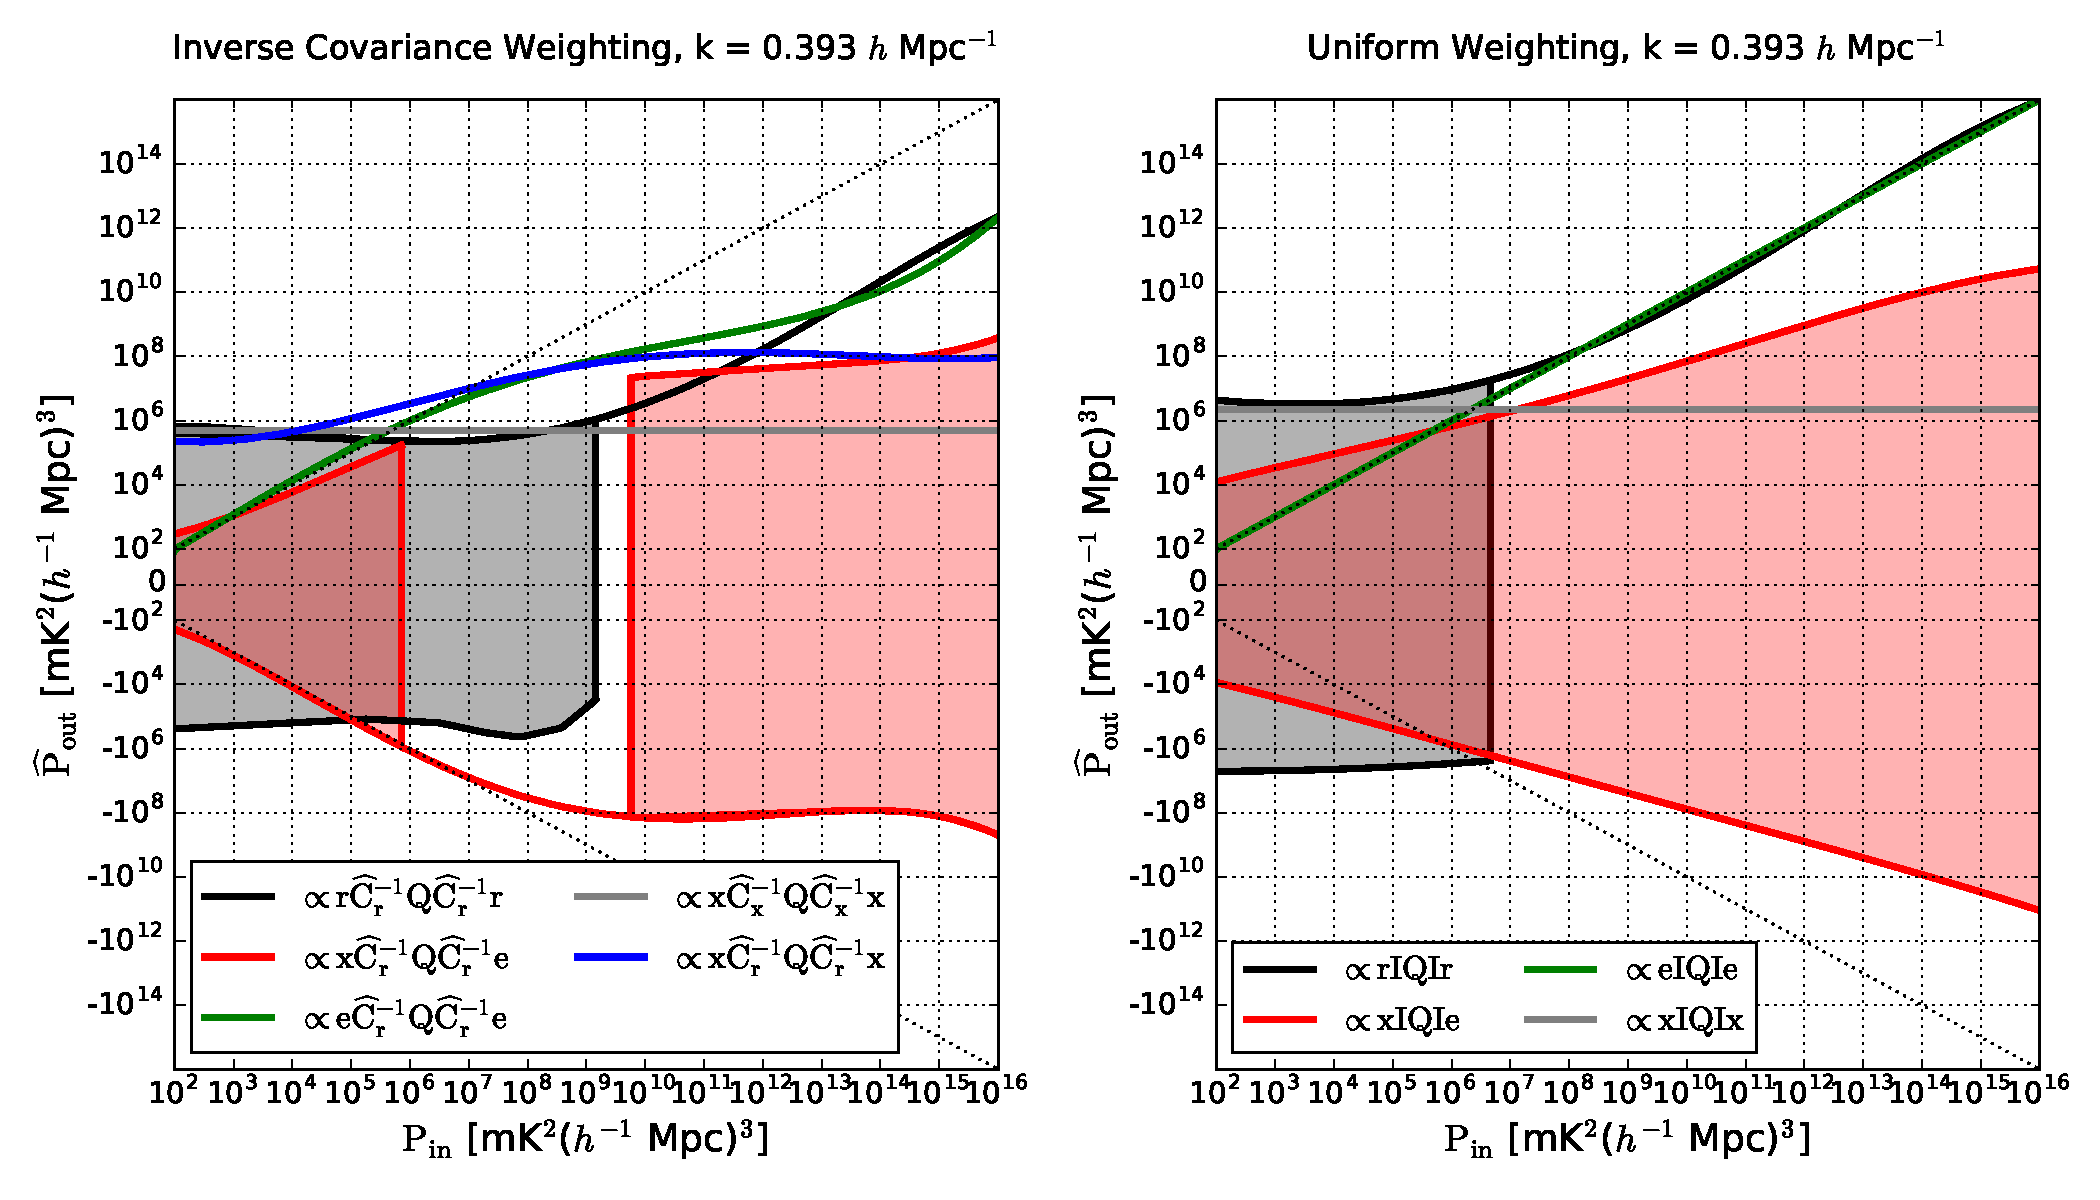
\includegraphics[width=1\textwidth]{plots/sigloss_terms.pdf}
	\caption{Illustration of the power spectrum amplitude of five different power spectrum terms, each a function of visibility data ($\textbf{x}$), simulated injected EoR signal ($\textbf{e}$), or both ($\textbf{r}$). This figure shows how these quantities behave as the power level of the injected EoR signal increases (along the x-axis).  The details of the simulation used to generate the figure is explained in Section \ref{sec:Practice}; here we sample a larger $P_{\rm in}$ range and fit smooth polynomials to our data points to make an illustrative example. We emphasize that the output power spectrum in black ($\widehat{P}_{\rm out}=\widehat{\textbf{P}}_r$) approximates the (lossy) power spectrum estimate that is output by our analysis pipeline prior to any signal loss adjustments. Roughly speaking, it can be compared to the input signal level ($P_{\rm in}$) to estimate the amount of signal loss. Left: Empirical inverse covariance weighting is used in power spectrum estimation, as done in \citetalias{ali_et_al2015}. The dotted diagonal black line indicates perfect 1:1 input-to-output mapping (no signal loss). The gray horizontal line is the power spectrum value of data alone, $\widehat{\textbf{P}}_{x}$ (it does not depend on injected power). The green signal-signal component is the term used in \citetalias{ali_et_al2015} to estimate signal loss. It is significantly higher than $\widehat{\textbf{P}}_{r}$ (black) when the cross-terms (red) are large and negative (black $=$ green $+$ red $+$ blue). In the regime where cross-correlations between signal and data are not dominant (small and large $P_{\rm in}$), the cross-terms have a noise-like term with width $\sqrt{\widehat{\textbf{P}}_e}\sqrt{\widehat{\textbf{P}}_x}$. However, at power levels comparable to the data (the middle region), the cross-terms can produce large, negative estimates due to couplings between $\textbf{x}$ and $\textbf{e}$ which affect $\widehat{\textbf{C}}_{r}$. This causes the difference between the green curve (which exhibits negligible loss at the data-only power spectrum value) and the black curve (which exhibits $\sim4$ orders of magnitude of loss). Right: The same power spectrum terms illustrated for the uniform weighted case.}
\label{fig:sigloss_terms}
\end{figure*}

The source of the strong negative cross-term is not immediately obvious, however it is an explainable effect. 
When $\textbf{R}_{r}$
is taken to be $\widehat{\textbf{C}}_{r}^{-1}$, the third term of Equation \eqref{eq:crossterm} is a cross-correlation between $\widehat{\textbf{C}}_{r}^{-1}\textbf{x}$ and
$\widehat{\textbf{C}}_{r}^{-1}\textbf{e}$. As shown in \citet{switzer_et_al2015}, this cross-correlation term is non-zero, and in fact negative in expectation. 
This negative cross-term power arises from a coupling between the inverse of 
$\widehat{\textbf{C}}_{r}$ and $\mathbf{x}$. 
Intuitively, we can see this by expanding the empirical covariance of $\textbf{r}=\textbf{x}+\textbf{e}$:

\begin{eqnarray}
\widehat{\textbf{C}}_{r} &=& \langle \textbf{rr}^{\dagger} \rangle_{t} \nonumber \\ 
&=& \langle \textbf{xx}^{\dagger} \rangle_{t} + \langle \textbf{xe}^{\dagger} \rangle_{t} + \langle \textbf{ex}^{\dagger} \rangle_{t} + \langle 
\textbf{ee}^{\dagger} \rangle_{t},
\end{eqnarray}

\noindent where we can neglect the first term because $\textbf{x}$ is small (i.e., the large negative cross-term power in the left panel of Figure \ref{fig:sigloss_terms} occurs when the injected amplitude surpasses the level of the data-only power spectrum).  Without loss of generality, we will assume
an eigenbasis of $\textbf{e}$, so that $\langle 
\textbf{ee}^{\dagger} \rangle_{t}$ is diagonal. The middle 
two terms, however, can have power in their off-diagonal terms due to the fact that, when averaging over a finite
ensemble, $\langle\textbf{xe}^\dagger\rangle_t$ is not zero.  As shown in Appendix C of \citet{parsons_et_al2014}%\footnote{This same appendix also gives a now-prescient warning about signal loss and the dangers of noise and sample variance in inverse covariance.}
, to leading order the inversion of a diagonal-dominant matrix like $\widehat{\textbf{C}}_{r}$ (from $\langle 
\textbf{ee}^{\dagger} \rangle_{t}$) with smaller
off-diagonal terms results in a new diagonal-dominant matrix with negative off-diagonal terms. These off-diagonal
terms depend on both $\textbf{x}$ and $\textbf{e}$. Then, when $\widehat{\textbf{C}}^{-1}_{r}$ is multiplied into $\textbf{x}$,
the result is a vector that is similar to $\textbf{x}$ but
contains a residual correlation to $\textbf{e}$ from the off-diagonal components of $\widehat{\textbf{C}}^{-1}_{r}$. The
correlation is negative because the product $\widehat{\textbf{C}}_r^{-1}\textbf{x}$ effectively squares the $\textbf{x}$-dependence
of the off-diagonal terms in $\widehat{\textbf{C}}^{-1}_{r}$ while retaining the negative sign that arose from the inversion
of a diagonal-dominant matrix.
% XXX [ARP: we may want to write this all out explicitly in an appendix]

%The correlation between $\widehat{\textbf{C}}_r^{-1}\textbf{e}$ and $\widehat{\textbf{C}}_r^{-1}\textbf{x}$ means that we cannot compute signal loss using a signal-only 
%simulation, which would yield greater values for $\widehat{P}_{\rm out}$ and thereby underestimate signal loss. This argument is also made in \citet{switzer_et_al2015} in regards to estimating loss associated with the foreground cleaning of Green Bank Telescope (GBT) data. Therefore, in our revised 
%signal loss computation we use the full quantity for $\widehat{P}_{\rm out}$ as defined in Equation \eqref{eq:crossterm_full}.
%weighted power spectrum of the data from the weighted power spectrum of data plus EoR. 

%\dcj{This paragraph has me confused.}
%The conclusion is that signal loss generically arises because of couplings between $\widehat{\textbf{C}}^{-1}_{r}$ and $\mathbf{x}$. In principle, using $\widehat{\textbf{C}}^{-1}_{r}$ in place of the true inverse covariance $\textbf{C}^{-1}$ provides yet another source of multiplicative bias, which results in a modification to the treatment shown here. Such a modification is accounted for in the demonstration of Appendix \ref{sec:sigloss_appendix}, where we additionally discard the assumption that $|\textbf{x}|\ll|\textbf{e}|$. However, despite the loosening of these approximations, one sees that the qualitative message (of anti-correlations resulting in signal loss) remains intact.

{\bf In general:} Another way to phrase the shortcoming of the empirical inverse covariance estimator is that it is not properly normalized. Signal loss due to couplings between the data and its weightings arise because our unnormalized quadratic estimator from Equation \eqref{eq:qhat} ceases to be a quadratic quantity, and instead contains higher order powers of the data. However, the normalization matrix $\mathbf{M}$ is derived assuming that the unnormalized estimator is quadratic in the data. The power spectrum estimate will therefore be incorrectly normalized, which manifests as signal loss. We leave a full analytic solution for $\mathbf{M}$ for future work, since our simulations already capture the full phenomenology of signal loss and have the added benefit of being more easily generalizable in the face of non-Gaussian systematics.

\subsection{Signal Loss in Practice}
\label{sec:Practice}

We now shift our attention towards computing upper limits on the EoR signal for the fringe-rate filtered PAPER-64 dataset in a way that accounts for signal loss. While our methodology 
outlined below is independent of weighting scheme, here we demonstrate the computation using empirically estimated inverse covariance weighting 
($\textbf{R} \equiv \widehat{\textbf{C}}^{-1}$), the weighting scheme used in \citetalias{ali_et_al2015} which leads to substantial loss. %With this weighting, our 
%expressions for $\widehat{P}_{\rm in}$ and $\widehat{P}_{\rm out}$ become:

%\begin{eqnarray}
%\widehat{P}_{\rm in}^{\alpha} &=&  \text{M}^{\alpha}_{\rm in}\textbf{e}^{\dagger}\textbf{I}\textbf{Q}^{\alpha}\textbf{I}\textbf{e} \\
%\widehat{P}_{\rm out}^{\alpha} &=&  \text{M}^{\alpha}_{r}\textbf{r}^{\dagger}\widehat{\textbf{C}}_{r}^{-1}\textbf{Q}^{\alpha}%\widehat{\textbf{C}}_{r}^{-1}\textbf{r}.% \nonumber \\
%\end{eqnarray}

%The treatment we outlined in the previous section implicitly assumed that signal loss corrections could be treated in expectation. In practice, however, the signal loss itself is a random variable --- some realizations of the cosmological signal may be more correlated with foreground modes than others, leading to more signal loss. This leads to two issues. The first is that Equation \eqref{eq:LinearPspecSum} may not hold. In particular, a third term that is a quadratic combination of $\f$ and $\s$ (e.g., $\f^\dagger \C^{-1} \s$) may appear. However, we can circumvent this issue by decomposing $\f$ into a sum of two vectors, one that is proportional to $\s$ and one that is orthogonal to $\s$. The former can be absorbed into the EoR term (part of the signal loss estimate), while the latter can be absorbed into the foreground term. In other words, suppose that we have
%\begin{equation}
%\phat_x \approx \ell_{\rm fg} |\mathbf{f}|^2 + \ell_{\rm eor} |\mathbf{e}|^2 + \ell_{\rm fe} \mathbf{f} \cdot \mathbf{e}.
%\end{equation}
%in place of Equation \eqref{eq:LinearPspecSum}. Now, split $\mathbf{f}$ into $\mathbf{ f}_\parallel +\mathbf{ f}_\perp$, which are the components of the foregrounds that couple to the EoR versus those that do not. Further parameterize $\mathbf{ f}_\parallel \equiv \rho \mathbf{e}$, where $\rho$ is some correlation coefficient that quantifies the degree of correlation between the foregrounds and the EoR. This then gives
%\begin{equation}
%\label{eq:fperpfpara}
%\phat_x \approx \ell_{\rm fg} |\mathbf{f}|^2 +( \ell_{\rm eor} + \rho  \ell_{\rm fe} ) |\mathbf{e}|^2 + \ell_{\rm fe} \mathbf{f}\cdot \mathbf{f}_\perp.
%\end{equation}
%Since $|\mathbf{e}|^2$ would be a lossless estimate of the true EoR power spectrum, this expression recovers the linear relation between the true EoR power spectrum and the lossy estimate.
%\dcj{Wait what? I think you are saying essentially that some x can remain in Pout which is what we are seeing. Or is this some extra bit of method which has been added to the analysis...} \acl{I'm not sure that's what I'm saying. (And by ``I'm not sure" I don't mean it in the colloquial sense of ``you're not right and I'm just trying to be polite about it", but rather the literal sense of the phrase ``I'm not sure"). What I was trying to say was that if I wrote Equation \eqref{eq:LinearPspecSum} without the ensemble average, I could say
%\begin{equation}
%\phat_x \approx \ell_{\rm fg} f^2 + \ell_{\rm eor} e^2 + \ell_{\rm fe} fe.
%\end{equation}
%(Note that even this is an approximation. In principle there is an infinite series containing all possible powers of 
%$e$ and $f$). Now, we split $f$ into $ f_\parallel + f_\perp$, which are the components of the foregrounds that 
%couple to the EoR versus those that do not. Further parameterize $f_\parallel \equiv \rho e$, where $\rho$ is 
%some correlation coefficient that quantifies the degree of correlation between the foregrounds and the EoR. 
%Under this parameterization, one can write the $fe$ term in terms of $e^2$ (which gets absorbed into the other 
%EoR term, plus residual foregrounds that we don't care about).}\acl{Just promoted this last part to something in 
%the main text.}\dcj{I will admit to being a little lost here.  Doesn't changing the basis just convert the unknown f 
%dot s term into other unknown terms. Isn't the whole point of Eq 24 supposed to be that we can subtract off the 
%$g(x)$ to estimate $\hat{\ell}_{\rm eor}$?  How do we subtract off $f\dot f_\perp$? Don't we want to know $
%\ell_{\rm eor}$ not $(\ell_{\rm eor} + \rho\ell_{\rm fe})$? }
%\acl{I think what we are trying to say here is that actually the thing we want \emph{is} $(\ell_{\rm eor} + \rho\ell_{\rm fe})$. Essentially, the potential coupling between the injected EoR and the foregrounds means that we lose the nice form of Equation \eqref{eq:LinearPspecSum}, which justified what is basically a multiplicative correction to signal loss. What we are suggesting here is that even when there is a coupling, the estimator can be parameterized as $\alpha  |\mathbf{e}|^2 + \beta$. So essentially we are defining an effective $
%\ell_{\rm eor}$, which is given by $(\ell_{\rm eor} + \rho\ell_{\rm fe})$.}

One issue to address is how one incorporates the randomness of $\widehat{P}_{\rm out}$ into our signal loss corrections. A different realization of the mock EoR signal is injected with each bootstrap run, causing the output to vary in three ways ---  there is noise variation from the bootstraps, there is cosmic variation from generating multiple realizations of the mock EoR signal, and there is a variation caused by whether the injected signal looks more or less ``like'' the data (i.e., how much coupling there is, which affects how much loss results). 

For each injection level, the true $P_{\rm in}$ is simply the average of our bootstrapped estimates $\widehat{P}_{\rm in}$, since $\widehat{P}_{\rm in, \alpha}$ is by construction an unbiased estimator. Phrased in the context of Bayes' rule, we wish to find the posterior probability distribution $p(P_{\rm in} | 
\widehat{P}_{\rm out})$, which is the probability of $P_{\rm in}$ given the uncorrected/measured power spectrum estimate $\widehat{P}_{\rm out}$.  Bayes' rule relates the posterior, which we don't know, to the likelihood, which we can forward model. In other words,

\begin{equation}
\label{eq:Bayes}
p(P_{\rm in} | \widehat{P}_{\rm out}) \propto {\mathcal{L} (  \widehat{P}_{\rm out} | P_{\rm in})}\,p(P_{\rm in}) ,
\end{equation}

\noindent where $\mathcal{L} $ is the likelihood function defined 
as the distribution of data plus signal injection ($\widehat{P}_{\rm out}$) given the injection $P_{\rm in}$.  We construct this distribution  
by fixing $P_{\rm in}$ and simulating our analysis pipeline for many realizations of the injected EoR signal 
consistent with this power spectrum. The resulting distribution is normalized such that the sum over $\widehat{P}_{\rm out}$ is unity, and the 
whole process is then repeated for a different value of $P_{\rm in}$. 

%\subsubsection{Signal Loss Implementation Details}
%\label{sec:Implementation}

The implementation details of the injection process require some more detailed explanation. In our code, we add a new realization of EoR to each independent bootstrap of data (see Section \ref{sec:Boot} for a description of PAPER's bootstrapping routine) with the goal of simultaneously capturing cosmic variance, noise variance, and signal loss. To limit computing time we perform $20$ realizations of each $P_{\rm in}$ level. We also run $50$ total EoR injection levels, yielding $P_{\rm in}$ values that range from $\sim$$10^{5}$\,mK$^{2}$ ($h^{-1}$ Mpc)$^{3}$ to $\sim$10$^{11}$\,mK$^{2}$ ($h^{-1}$ Mpc)$^{3}$, resulting in a total of $1000$ data points on our $P_{\rm in}$ vs. $\widehat{P}_{\rm out}$ grid. 

Going forward, we treat every $k$-value separately in order to determine an upper limit on the EoR signal per $k$. We bin our simulation outputs along the $P_{\rm in}$ axis (one bin per injection level) and, since they are well-approximated by a Gaussian distribution in our numerical results, we smooth the distribution of $\widehat{P}_{\rm out}$ values by fitting Gaussians for each bin based on its mean and variance (and normalize them). Stitching all of them together results in a 2-dimensional transfer function --- the likelihood function in Bayes' rule, namely $\mathcal{L} (  \widehat{P}_{\rm out} | P_{\rm in})$. We then have a choice for our prior, $p(P_{\rm in})$, and we choose to invoke a Jeffreys prior (\citealt{jaynes1968}) because it is a true uninformative prior. %For a derivation and more details about the Jeffreys prior used in our analysis, see Appendix \ref{sec:jeffreys}.

Finally, our transfer functions are shown in Figure \ref{fig:sigloss_transfercurve} for both the weighted (left) and unweighted (right) cases. Our bootstrapped power spectrum outputs are shown as black points and the colored heat-map overlaid on top is the likelihood function modified by our prior. Although we only show figures for one $k$-value, we note that 
the shape of the transfer curve is similar for all $k$'s. We then invoke Bayes' interpretation and re-interpret it as the posterior $p(P_{\rm in}|\widehat{P}_{\rm out})$ where we recall that $\widehat{P}_{\rm out}$ represents a (lossy) power spectrum. To do this we make a horizontal cut across at the data value $\widehat{\textbf{P}}_{x}$ (setting $\widehat{P}_{\rm out} = \widehat{\textbf{P}}_{x}$), shown by the gray solid line, to yield a posterior distribution for the signal. We normalize this final distribution and compute the $95\%$ confidence interval (an upper limit on EoR).

%We note that the distribution of $\phat_{x}$ has a variance determined from the bootstrapping process and is peaked around the power spectrum value computed from the no-bootstrapping case. We smooth its distribution using 1D kernel density estimators (and normalize to unity) before multiplying it with the transfer function. Performing a summation and normalization for the entire distribution of $\phat_{x}$ yields a final $P_{\rm in}$ distribution --- the distribution of our data as seen through the signal loss lens. We compute power spectrum points from the peak of the histograms, and power spectrum errors from $95\%$ confidence intervals. 

By-eye inspection of the transfer function in Figure \ref{fig:sigloss_transfercurve} gives a sense of what the signal loss result should be. The power spectrum value of our data, $
\widehat{\textbf{P}}_{x}$ is marked by the solid gray horizontal lines. From the left plot (empirically estimated inverse covariance weighting), one can eyeball that a data value of $10^{5} \,$mK$^{2}$ ($h^{-1}$ Mpc)$^{3}$, for example, would map approximately to an upper limit of $\sim10^{9} \,$mK$^{2}$ ($h^{-1}$ Mpc)$^{3}$, implying a signal loss factor of $\sim10^{4}$. 

%As a final complication to our procedure, we note that there will be some scatter in our likelihood due to our having only a finite number of simulations. Ideally, running many simulations would lead to convergence; however, our desire to be able to quickly and easily estimate signal loss for a variety of weighting schemes and datasets means having a finite sample in practice. \dcj{This dependence on injection count was checked with a run having 10x the usual number of integrations.} To separate the intrinsic stochasticity of signal loss from that which arises due to simulation sample variance, we repeat our analysis for a power spectrum estimator without signal loss ($\textbf{R} = \textbf{I}$), shown as the right plot in Figure \ref{fig:sigloss_transfercurve}. Here the scatter, evident as deviations from unity-transfer, is entirely due to finite sample variance. To remove this effect we measure the width of this lossless case and then de-convolve that extra width from the likelihood for the lossy scenario. Specifically, we de-convolve Gaussian distributions of $\widehat{P}_{\rm out}$ in the uniform-weighted case from those of the weighted case (vertical cuts through the plots in Figure \ref{fig:sigloss_transfercurve}), for every $P_{\rm in}$. By doing this, we are left with only the intrinsic scatter in signal loss, or scatter that stems from how much the random EoR signal $\textbf{e}$ happens to 
%look like the data $\textbf{x}$, a quantity we do not know offhand but one that we would like to correct for. As an extreme example, if we are very unlucky, one realization of $\textbf{e}$ would have the same shapes, or eigenvectors, as $\textbf{x}$. An empirically-derived covariance would then down-weight these shapes, destroying the entire EoR signal. On the other hand, the less that $\textbf{e}$ looks like $\textbf{x}$, the less signal loss that would result. The intrinsic scatter we can get is not a dominant factor in this case but it is important to correct for the fact that a particular $\widehat{P}_{\rm out}$ value could arise from a range of $P_{\rm in}$ values. 

%The solid black diagonal line in Figure \ref{fig:sigloss_transfercurve} shows unity-transfer, which we expect to occur for the 
%nweighted case ($\textbf{R} = \textbf{I}$). Therefore, it is worth thinking about the spread, or scatter, around this black line that 
%we see in the right plot (the colored `heat-map'). One might imagine that there should be one true $\widehat{P}_{\rm out}$ value for every 
%$P_{\rm in}$, implying one well-determined signal loss factor for every data value. Focusing on the unweighted case alone, the 
%scatter observed arises from the fact that the values of the cross-terms involving $\textbf{e}$ and $\textbf{x}$ in Equation 
%\eqref{eq:pout_expand} change for different mock EoR signals, $\textbf{e}$. Since we draw different random $\textbf{e}$'s for 
%every bootstrap (for reasons made clear in the next paragraph), there is a range of $\widehat{P}_{\rm out}$ values that results from the same 
%$P_{\rm in}$. This randomness causes the spread seen in the right plot of Figure \ref{fig:sigloss_transfercurve}, as well as most of 
%the spread in the weighted case (left plot).

\begin{figure*}
	\centering
	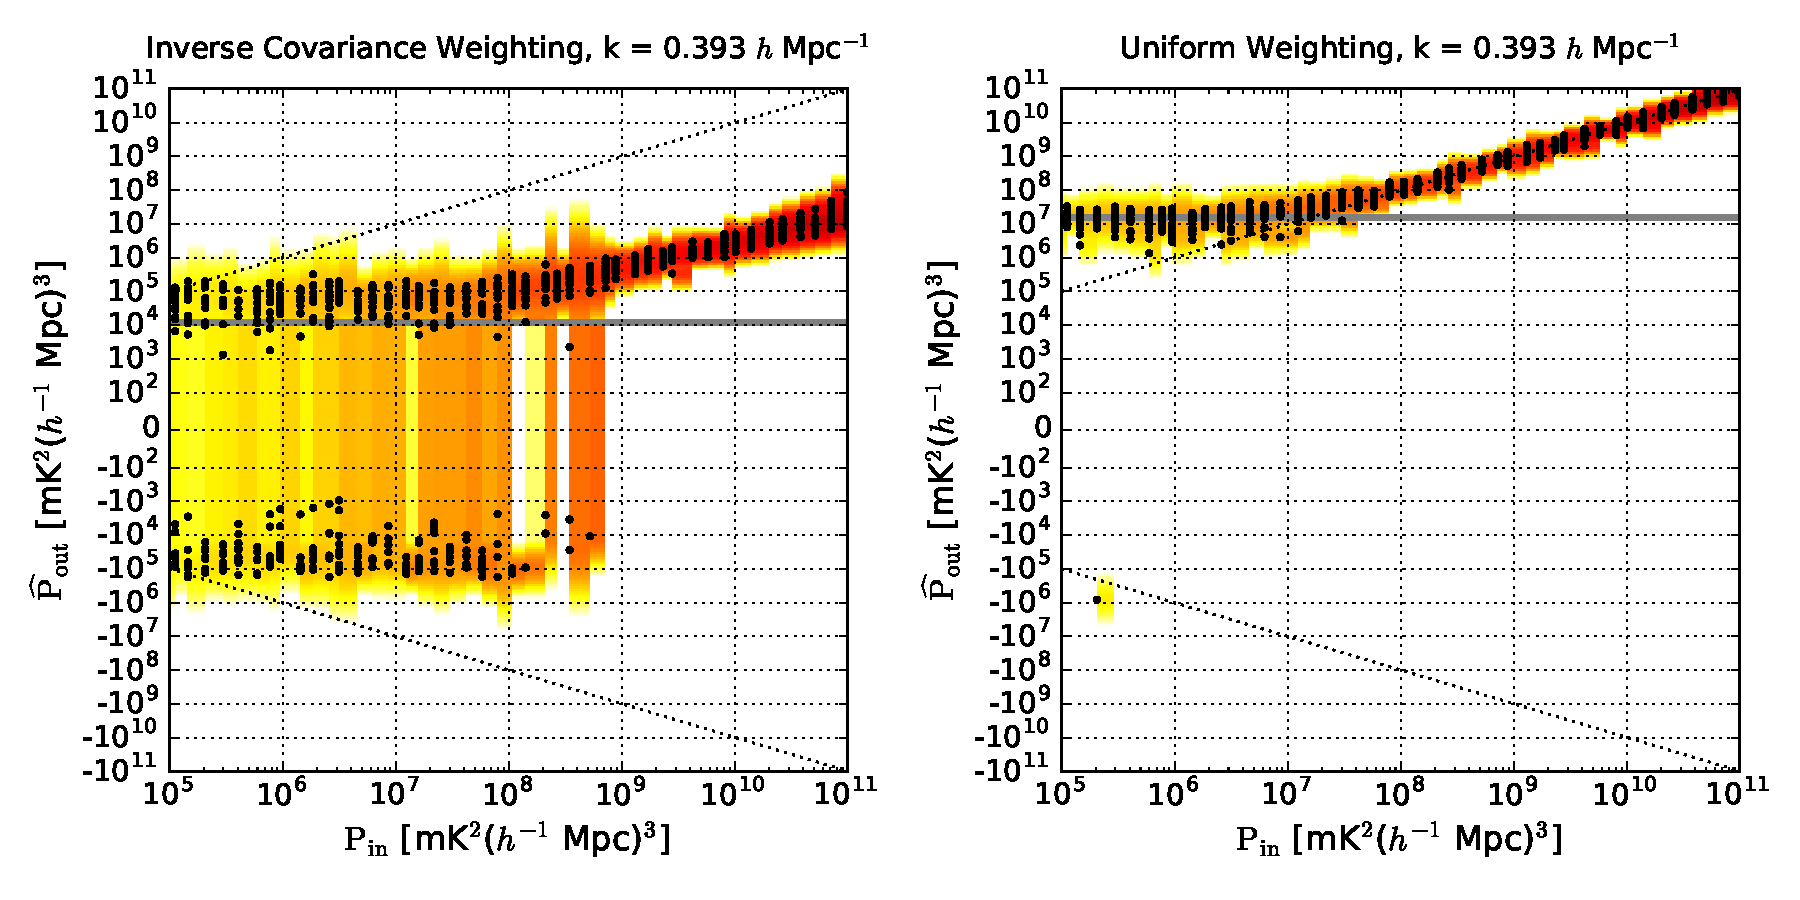
\includegraphics[width=1\textwidth]{plots/sigloss_transfercurve_posneg.pdf}
	\caption{Signal loss transfer functions showing the relationship of $P_{\rm in}$ and $\widehat{P}_{\rm out}$, as defined by Equations \eqref{eq:Pin} and \eqref{eq:sigloss}. Power spectra values (black points) are generated for $20$ realizations of $\textbf{e}$ per signal injection level. Since our $\widehat{P}_{\rm out}$ values are well-approximated by a Gaussian distribution, we fit Gaussians to each injection level based on the mean and variance of the simulation outputs. This entire likelihood function is then multiplied by a Jeffreys prior for $p(P_{\rm in}$), with the final result shown as the colored 
heat-maps on top of the points. Two cases are displayed: empirically estimated inverse covariance weighted PAPER-64 data (left) and uniform-weighted data (right). The dotted black 
diagonal lines mark a perfect unity mapping, and the solid gray horizontal line denotes the power spectrum value of the data $\widehat{\textbf{P}}_{x}$, from which a posterior distribution for the signal is extracted. From these plots, it is clear that the weighted case results in $\sim4$ orders of magnitude of signal loss at the data-only power spectrum value, whereas the uniform-weighted case does 
not exhibit loss. The general shape of these transfer functions are also shown by the black curves in Figure \ref{fig:sigloss_terms} for comparison.}
	\label{fig:sigloss_transfercurve}
\end{figure*}

%One peculiar aspect of Figure \ref{fig:sigloss_transfercurve} is the fact that at low $P_{\rm in}$ values it appears that we can have signal gain ($\widehat{P}_{\rm out} > P_{in}$). \cc{This is a log-plotting effect and is under-construction!}.
%This is unphysical in nature but caused due to the dominating cross-terms involving $\textbf{e}$ and $\textbf{x}$ in Equation \eqref{eq:pout_expand} once $\textbf{e}$ becomes small. 
%
%The shape of our signal loss transfer function can be described as follows. At low injection levels, for small $\textbf{e}$, we are dominated by the cross-terms involving $\textbf{e}$ and $\textbf{x}$ in Equation \eqref{eq:pout_expand}. As $\textbf{e}$ increases, we move 
%into a regime where $\widehat{P}_{\rm out} \sim P_{in}$, and then eventually into a regime where $\widehat{P}_{\rm out} < P_{in}$ when $\textbf{e}$ is 
%large enough to be destroyed if weighting the data using itself. Although we only show figures for one $k$ value, we note that 
%the shape of the transfer curve is nearly identical for all $k$'s (though we treat each $k$ separately).

%\begin{figure*}
%	\centering
%	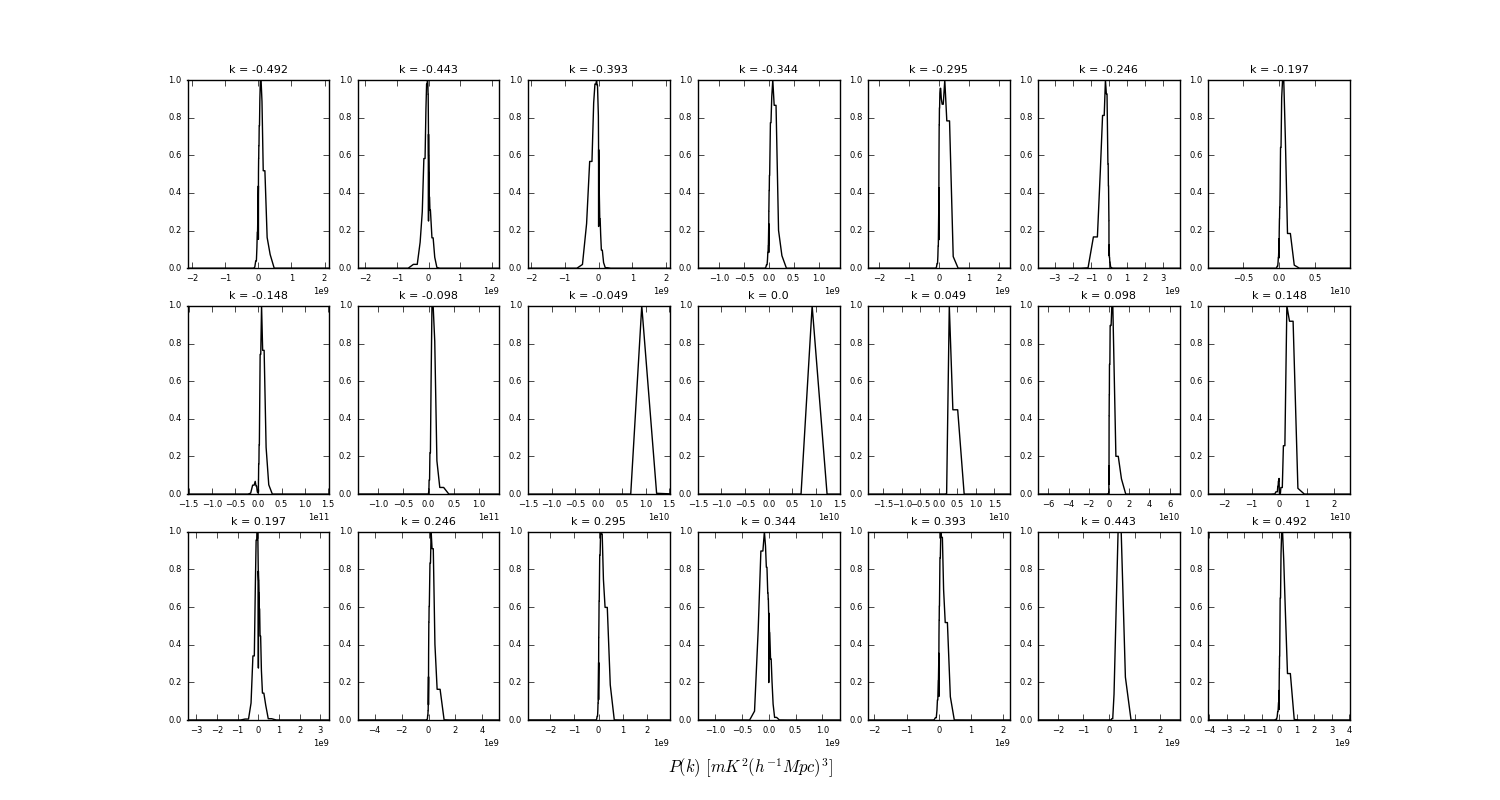
\includegraphics[trim={1cm 0cm 1cm 1cm},width=1\textwidth]{plots/sigloss_datadist_inversecovariance.png}
%	\caption{Normalized histograms of the power spectra that result from using inverse covariance weighting on %PAPER-64 data after signal loss correction. Power spectrum points are computed from the peak of the distributions. Errors are computed using $95\%$ confidence intervals.}
%	\label{fig:sigloss_datadist_inversecovariance}
%\end{figure*}

The loss-corrected power spectrum limit for empirically estimated inverse covariance weighted PAPER-64 data is shown in Figure \ref{fig:ps2_data} (solid red), which we can compare to the original lossy result (dashed red). %There are a few important checks to examine. First, we see that the uniform-weighted power spectrum $2\sigma$ upper limit (dashed blue) is identical in both panels. This is an important check, as we expect no signal loss for this case. Any difference here would indicate an error in the pipeline or discrepancy in the range of data included. Additionally, it is clear that the power spectrum, prior to signal loss estimation, is inconsistent with the (now revised) theoretical noise level prediction. 
Post-signal loss estimation, the power spectrum limits are higher than both the theoretical noise level (green) and uniform-weighted power spectrum (which is shown three ways: black and gray points are positive and negative power spectrum values, respectively, with $2\sigma$ error bars from bootstrapping, the solid blue is the upper limit on the EoR signal using the full signal injection framework, and the shaded gray is the power spectrum values with thermal noise errors). We elaborate on this point in the next section, as well as investigate alternate 
weighting schemes to inverse covariance weighting, with the goal of finding one that balances the aggressiveness of down-weighting contaminants and minimizing the loss of the EoR signal. 

\begin{figure*}
	\centering
	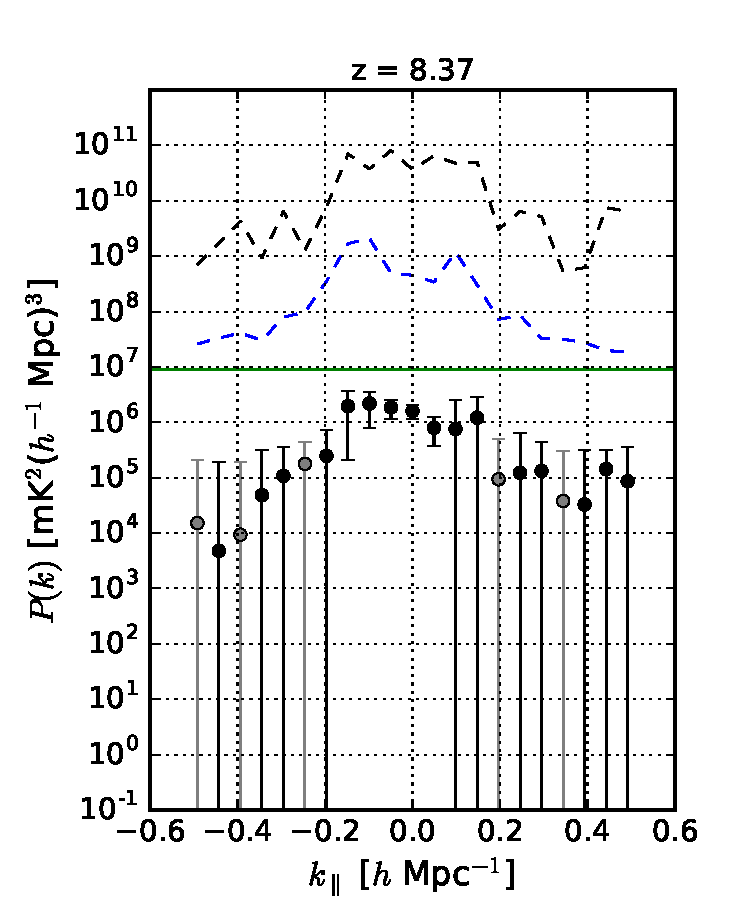
\includegraphics[width=0.4\textwidth]{plots/ps1_data.pdf}
	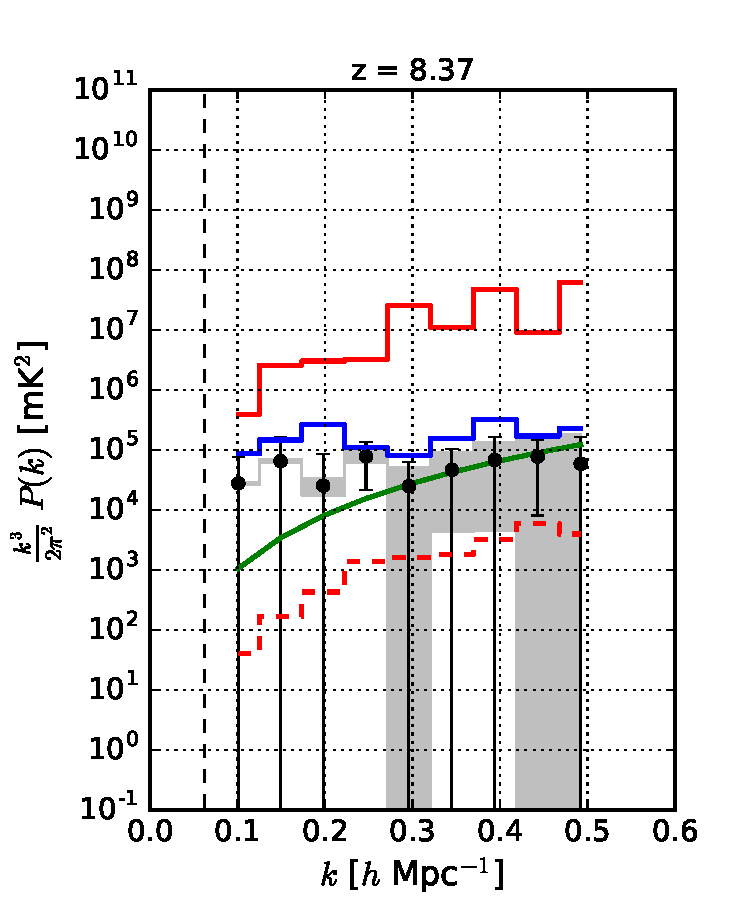
\includegraphics[width=0.4\textwidth]{plots/ps2_data.pdf}
	\caption{A power spectrum of a subset of PAPER-64 data illustrating the use of empirical inverse covariance weighting. The solid red curve is the $2\sigma$ upper limit on the EoR signal estimated from our signal injection framework using empirical inverse covariance weighting. Shown for comparison is the lossy limit prior to signal loss estimation (dashed red). The theoretical $2\sigma$ thermal noise level prediction based on observational parameters is in green, whose calculation is detailed in Section \ref{sec:Error}. Additionally, the power spectrum result for the uniform weighted case is shown in three different ways: power spectrum values (black and gray points as positive and negative values, respectively, with $2\sigma$ error bars from bootstrapping), the $2\sigma$ upper limit on the EoR signal using our full signal injection framework (solid blue), and the measured power spectrum values with $2\sigma$ thermal noise errors (gray shaded regions). The vertical dashed black lines signify the horizon limit for this analysis using $30$\,m baselines. In this example, we see that the lossy power spectrum limit is $\sim 4$ orders of magnitude too low when using empirical inverse covariance weighting.}
\label{fig:ps2_data}
\end{figure*}


\subsection{Minimizing Signal Loss}
\label{sec:Weight}

With a signal loss formalism established, we now have the capability of experimenting 
with different weighting options for $\textbf{R}$. Our goal here is to choose a weighting method that successfully down-weights 
foregrounds and systematics in our data without generating large amounts of signal loss as we have seen with the inverse covariance estimator. We have found that the balance 
between the two is a delicate one and requires a careful understanding and altering of empirical covariances. 

We saw in Section \ref{sec:otherweight} how limiting the number of down-weighted eigenmodes (i.e., flattening out part of the 
eigenspectrum and effectively decoupling the lowest-valued eigenmodes, which are typically EoR-dominated, from the data) can help minimize signal loss. We experiment with this idea on PAPER-64 data, dialing the number of modes 
that are down-weighted from zero (which is equivalent to identity-weighting, or the uniform-weighted case) to $21$ (which is the full inverse 
covariance estimator). The power spectrum results for one $k$-value, both before and after signal loss 
estimation, are shown in the top panel in Figure \ref{fig:sigloss_modeloop}. We see that the amount of signal loss increases as weighting 
becomes more aggressive (dashed red). In other words, more EoR-dominated fluctuations are being overfit and 
subtracted as more modes are down-weighted. We also find that the power spectrum upper limit, post-signal loss estimation, 
increases with the number of down-weighted modes (solid red). The more modes we use in down-weighting, the stronger the coupling between the weighting and the data, and the greater the error we have in estimating the power spectrum. \citet{switzer_et_al2013} took a similar approach in determining the optimal number of modes to down-weight in GBT data, finding similar trends and noting that removing too few modes is limited by residual foregrounds and removing too many modes is limited by large error bars and signal loss.

Optimistically, we expect there to be a ``sweet spot" as we dial our regularization knob; a level of regularization where weighting 
is beneficial compared to uniform weighting (blue). In other words, we would like a weighting scheme that down-weights eigenmodes that predominantly describe foreground modes, but not EoR modes. We see in Figure \ref{fig:sigloss_modeloop} that this occurs roughly when 
only the $\sim3$ highest-valued eigenmodes are down-weighted and the rest are given equal weights (though for the case shown, weighting only slightly outperforms uniform weighting). For a similar discussion on projecting out modes (zeroing out eigenmodes, rather than just ignoring their relative weightings as we do in this study), see \citet{switzer_et_al2013}. 

We also saw in Section \ref{sec:otherweight} how adding the identity matrix to the empirical covariance can minimize signal loss. We experiment with this idea as well, shown in the bottom panel of Figure \ref{fig:sigloss_modeloop}. The dashed red and solid red lines represent power spectrum limits pre and post-signal loss estimation, respectively, as a function of the strength of $\textbf{I}$ that is added to $\widehat{\textbf{C}}$, quantified as a percentage of Tr($\widehat{\textbf{C}})\textbf{I}$ added to $\widehat{\textbf{C}}$. We parameterize this ``regularization strength" parameter as $\gamma$, namely $\widehat{\textbf{C}} \equiv \widehat{\textbf{C}} + \gamma$Tr$(\widehat{\textbf{C}})\textbf{I}$. From this plot we see that only a small percentage of Tr($\widehat{\textbf{C}})$ is needed to significantly reduce loss. We expect that as the strength of $\textbf{I}$ is increased (going to the left), both the red curves will approach the uniform-weighted case. We also notice that the post-signal loss limit hovers around the uniform-weighted limit for a large range of regularization strengths and while an overall trend from high-to-low signal loss is seen as the strength increases, there does not appear to be a clear ``minimum" that produces the least loss.

\begin{figure*}
	\centering
	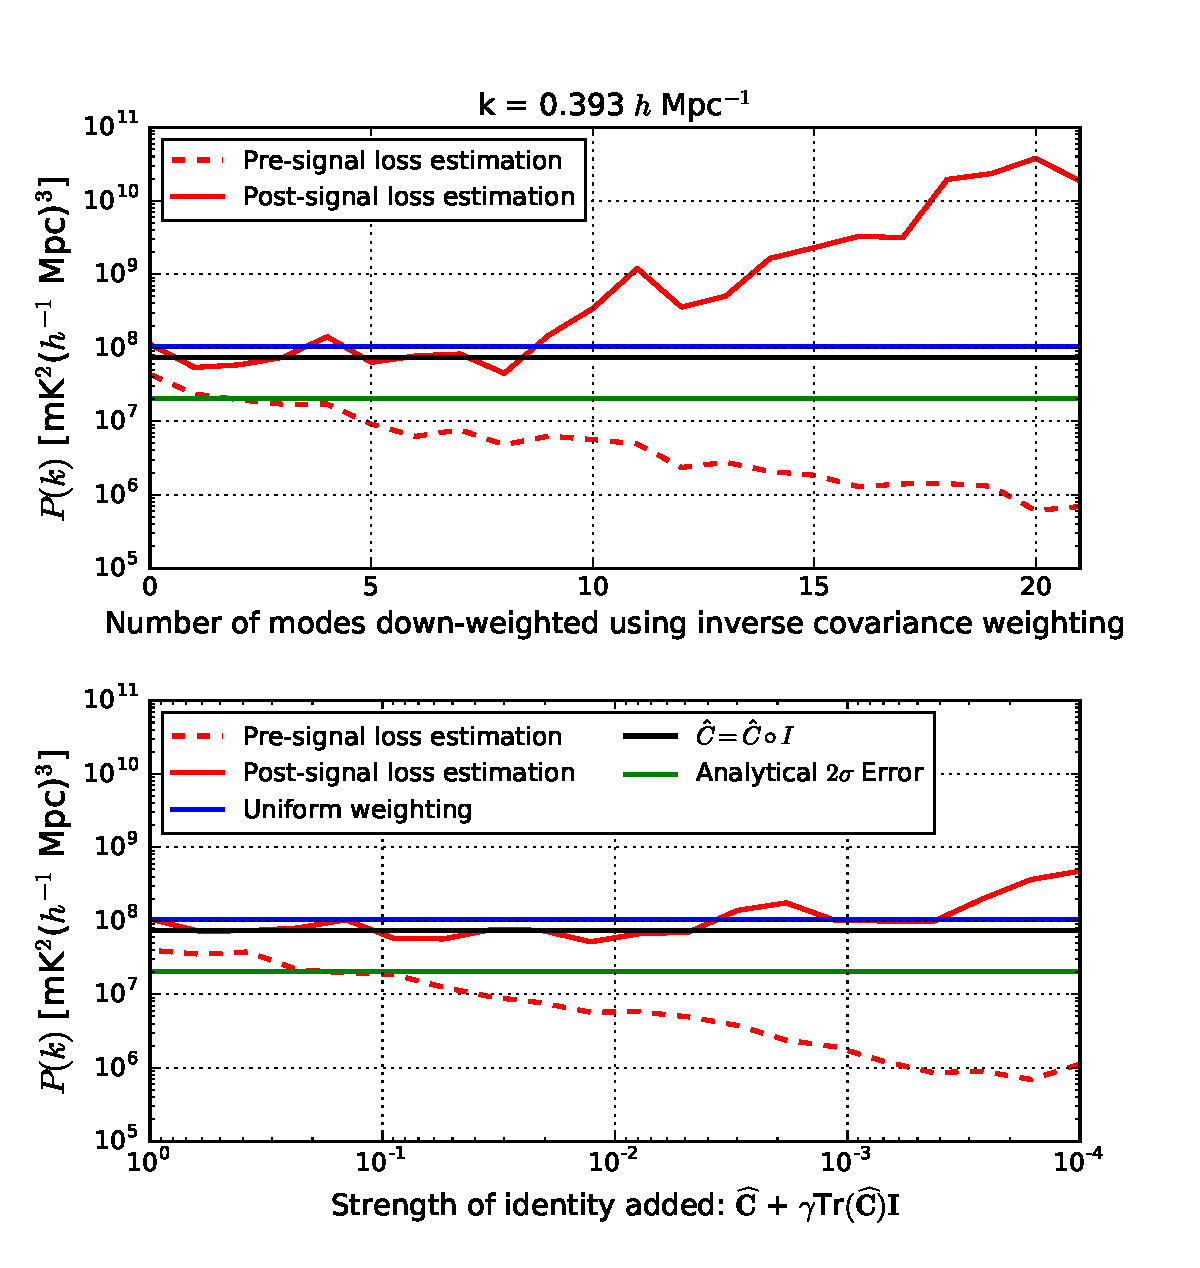
\includegraphics[width=1\textwidth]{plots/sigloss_modeloop_2panel.pdf}
	\caption{Power spectra $2\sigma$ upper limits for $k=0.393$\,$h$ Mpc$^{-1}$ for fringe-rate filtered PAPER-64 data. Top: Values 
are shown before (dashed red) and after (solid red) signal loss estimation via our signal injection framework as a function of number of eigenmodes of $\widehat{\textbf{C}}$ that 
are down-weighted. This regularization knob is tuned from $0$ modes on the left (i.e., unweighted) to $21$ modes on the right (i.e., the full inverse 
covariance estimator). $\sim4$ orders of magnitude of signal loss results when using empirically estimated inverse covariance weighting. Bottom: Power spectrum upper limits before (dashed red) and after (solid red) signal loss estimation as a function of identity added to the empirical covariance. This regularization knob is tuned from $\gamma = 10^{-4}$ on the right (i.e., very little regularization) to $\gamma = 1$ on the left (see main text for the definition of $\gamma$). Also 
plotted in both panels for comparison are $2\sigma$ power spectrum upper limits for the uniform-weighted case (blue) and inverse variance 
weighted case (black); both are after signal loss estimation. Finally, a theoretical prediction for noise ($2\sigma$ error) is plotted 
as green. In the PAPER-64 analysis in this paper, we choose to use a regularization scheme of $\widehat{\textbf{C}}_{\rm eff} \equiv 0.09 \, $Tr($\widehat{\textbf{C}})\textbf{I} + \widehat{\textbf{C}}$ ($\gamma = 0.09$) as a simple example of regularization that minimizes loss, and note that the power spectrum limits using this type of regularization are roughly constant across a large range of values of $\gamma$.}
	\label{fig:sigloss_modeloop}
\end{figure*}

In addition to our thermal noise prediction (green) and uniform-weighted power spectrum limit (blue), one additional horizontal line is shown in Figure \ref{fig:sigloss_modeloop} 
in both panels and represents a third regularization technique. This line (black) denotes the power spectrum value, post-signal loss estimation, for inverse variance weighting (multiplying an identity 
matrix element-wise to $\widehat{\textbf{C}}$). This result is single-valued and not a function of the horizontal axis. We see that all three regularization schemes shown (solid red top panel, solid red bottom panel, black) perform similarly at 
their best (i.e., when $\sim3$ eigenmodes are down-weighted in the case of the top panel's solid red curve). However, for the remainder of this paper, we choose to use the weighting option of $\widehat{\textbf{C}} + 0.09 \,$Tr($\widehat{\textbf{C}})\textbf{I}$, or $\gamma = 0.09$, which we will denote as $\widehat{\textbf{C}}_{\rm eff}$. We choose this weighting scheme merely as a simple example of regularizing PAPER-64 covariances, noting that the power spectrum upper limit remains roughly constant for a broad range of values of $\gamma$. 

It is important to note that our signal injection methodology for assessing loss makes the assumption that we know the true signal's strength and structure. Realistically, these details about the EoR signal are unknown and our signal loss framework is limited by our simulations. Therefore, while this paper employs this methodology as an example of one way of estimating loss, Kolopanis et al. (\textit{in prep.}) use uniform weightings in order to produce more trustworthy, straightforward power spectrum limits that do not suffer from loss.

The power spectrum result for our subset of PAPER-64 data (using only one baseline separation type, $10$ baselines, and $\widehat{\textbf{C}}_{\rm eff}$) using the analysis presented in this paper is shown in Figure 
\ref{fig:ps1_data}. Again, the solid red curve represents our upper limit on the EoR signal using the full signal injection framework. The uniform weighted case is shown as the black and gray points, which correspond to positive and negative power spectrum values respectively (with 
$2\sigma$ errors bars from bootstrapping). It is also shown as an upper limit using the signal injection framework (solid blue), which is interestingly larger than the errors computed from bootstrapping, likely because the full injection framework takes into account additional sample variance whereas the bootstrapped errors do not. Finally, the gray shaded regions combine the measured uniform weighted power spectrum values with thermal noise errors. We show this power spectrum result as one example of how a simple regularization of an empirical covariance matrix can minimize signal loss, though we also note that this weighting does not produce more stringent limits than the uniform weighted case, thus further motivating uniform-weighting for Kolopanis et al. (\textit{in prep.}). 

\begin{figure*}
	\centering
	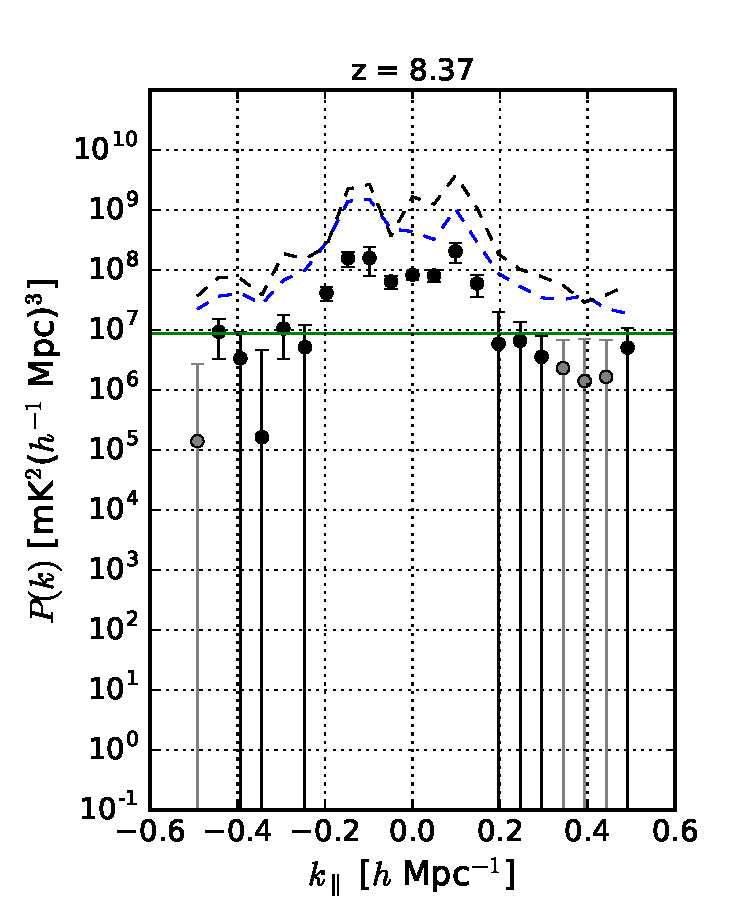
\includegraphics[width=0.4\textwidth]{plots/ps1_data_add.pdf}
	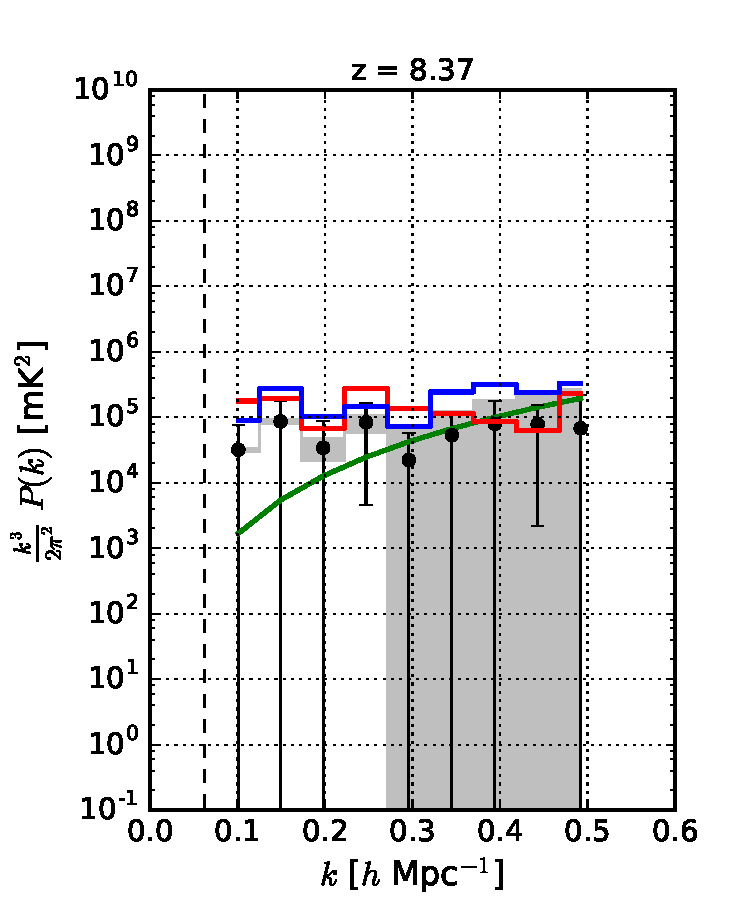
\includegraphics[width=0.4\textwidth]{plots/ps2_data_add.pdf}
	\caption{A power spectrum of a subset of PAPER-64 data illustrating the use of $\widehat{\textbf{C}}_{\rm eff}$ to minimize signal loss. The solid red curve is the $2\sigma$ upper limit on the EoR signal estimated from our signal injection framework. The theoretical $2\sigma$ thermal noise level prediction based on observational parameters is in green. Additionally, the power spectrum result for the uniform weighted case is shown in three different ways: power spectrum values (black and gray points as positive and negative values, respectively, with $2\sigma$ error bars from bootstrapping), the $2\sigma$ upper limit on the EoR signal using our full signal injection framework (solid blue), and the measured power spectrum values with $2\sigma$ thermal noise errors (gray shaded regions). The vertical dashed black lines signify the horizon limit for this analysis using $30$\,m baselines. This power spectrum result does not use the full dataset's sensitivity as in \citetalias{ali_et_al2015} and Kolopanis et al. (\textit{in prep.}), though we include all analysis changes which have mostly stemmed from revisions regarding signal 
loss, bootstrapping, and the theoretical error computation. We see that the regularization scheme used here produces limits similar to the unweighted limits.}
	\label{fig:ps1_data}
\end{figure*}

In this section we have shown three simple ways of regularizing $\widehat{\textbf{C}}$ to minimize signal loss using PAPER-64 
data. There are many other weighting schemes that we leave for consideration in future work. For example, one could estimate 
$\widehat{\textbf{C}}$ using information from different subsets of baselines. For redundant arrays this might mean calculating $
\widehat{\textbf{C}}$ from a different but similar baseline type, such as the $\sim30$\,m diagonal PAPER baselines (instead of the 
horizontal E/W ones). Alternatively, covariances could be estimated from all baselines except the two being cross-multiplied 
when forming a power spectrum estimate. This method was used in \citet{parsons_et_al2014} (a similar method was also used in \citet{dillon_et_al2015}) in order to avoid suppressing the 
21\,cm signal, and it is worth noting that the PAPER-32 results are likely less impacted from the issue of signal loss underestimation 
because of this very reason (however, they are affected by the error estimation issues described in Section \ref{sec:Error}, so 
we also regard those results as suspect and superseded by those of Kolopanis et al. (\textit{in prep.})).

Another possible way to regularize $\widehat{\textbf{C}}$ is to use information from different ranges of LST. For example, one could 
calculate $\widehat{\textbf{C}}$ with data from LSTs where foregrounds are stronger (earlier or later LSTs than the ``foreground-quiet" range typically used in forming power spectra) --- doing so may yield a better description of the foregrounds that we desire to 
down-weight, especially if residual foreground chromaticity is instrumental in origin and stable in time. Fundamentally, each of these examples are similar in that they rely on a computation of $\widehat{\textbf{C}}$ from 
data that is similar but not exactly the same as the data that is being down-weighted. Ideally this would be effective in down-weighting shared contaminants yet avoid signal loss from overfitting EoR modes in the power spectrum dataset itself. 

In Section \ref{sec:CaseStudy}, we have detailed several aspects of signal loss in PAPER-64: how the loss arises, how it can be estimated from an injection framework, and ways it can be minimized. We again emphasize that these lessons learned about signal loss are largely responsible for shaping our revised analysis of PAPER data. In the remainder of this paper, we will transition to other aspects of our analysis that have been revised since \citetalias{ali_et_al2015}.

% SECTION 4 OTHER ERRORS ---------------------------------------------------------------------------------

\section{Additional PAPER-64 Revisions}
\label{sec:OtherErrors}

Underestimated signal loss is the main reason for the revision of the power spectrum limits from \citetalias{ali_et_al2015}. It is interesting to note that --- had all the other aspects of the original analysis been correct --- the underestimated limits may have been more easily caught. Unfortunately, two related power spectrum components, namely the error bars on the power spectrum data points and the theoretical noise prediction, were also calculated incorrectly.

In this section, we summarize multiple inconsistencies and errors that have been found since the previous analysis in terms of error estimation. We first describe updated methods regarding bootstrapping, which determines the error bars on our limits. We then highlight an updated calculation for the theoretical noise sensitivity of PAPER-64 and illustrate how our revised calculation has been verified through simulations. 

\subsection{Bootstrapping}
\label{sec:Boot}

Broadly speaking, we desire robust methods for determining accurate 
confidence intervals for our measurements. For PAPER's analysis, we choose a data-driven method of error estimation, computing error bars that have been derived from the inherent 
variance of our measurements. A common technique used to do this is bootstrapping, which we first define below and then discuss its application to PAPER.

Bootstrapping uses sampling with replacement to estimate a posterior distribution. For example, bootstrap measurements (of power spectra, for example) can be made from different random samples of data. Each of these bootstraps is a different realization drawn from some underlying distribution, and realizations are correlated with each other to a degree set by the fraction of sampled points that are held in common between them. Through the process of re-sampling and averaging along different axes of a dataset, such as along baselines or times, we can estimate error bars for our results which represent the underlying distribution of values that are allowed by our measurements (\citealt{efron_tibshirani1994}; \citealt{andrae2010}).

%Suppose we have $N$ different measurements targeting the same quantity (for example, $N$ power spectrum measurements). Bootstrapping means that we form $N_{\rm boot}$ (often a large number) bootstraps, where each bootstrap is a random selection of the $N$ measurements. Bootstraps each have dimensions of $N$, and the values populated into each bootstrap are drawn from the original set of measurements with replacement (i.e., every $n^{th}$ slot in $N$ is filled randomly for each bootstrap). Next we take the mean of each bootstrap to collapse it from an array of length $N$ to a single number (we are interested in the mean statistic here, but any function of interest can be applied to each bootstrap as long as it's the same function for each one). The error (on the mean) is then computed as the standard deviation across all bootstraps. 

%We must be careful in distinguishing $N_{\rm boot}$, the number of bootstraps, from $N$, the number of samples, or elements, or values, that comprise a bootstrap. $N_{\rm boot}$ is typically large, and the standard deviation across bootstraps (the error we are computing) converges for large $N_{\rm boot}$. Typically $N$ is a straightforward value to set that just depends on the experiment (i.e., it is simply the number of samples along the axis that is being re-sampled). However, we will see that $N$ depends on sample independence, and it is this dependence that led to the underestimation of errors in \citetalias{ali_et_al2015}.

%Let us first suppose we have a Gaussian random signal dataset of length $N=1000$ and unity variance (zero mean). This could represent $1000$ power spectrum measurements, for which we are interested in its error. We predict that the error on the mean should obey $1/\sqrt{N}$, where $N$ is the number of samples.

%We next form $500$ bootstraps ($N_{\rm boot} = 500$). To create each bootstrap, we draw $N$ samples, with replacement, of the original data, and take the mean over the $N$ samples. The standard deviation over the $500$ bootstraps gives an error estimate for our dataset. This error is indicated by the gray star in Figure \ref{fig:toy_error1} and matches our theoretical prediction (green).

One major caveat of bootstrapping arises when working with correlated data. If, for example, a dataset has many repeated 
values inside it, this would be reflected in each bootstrap. The same value would be present multiple times within a bootstrap 
and also be present between bootstraps, purely because it has a more likely chance of being drawn if there are repeats of 
itself. Therefore, bootstrapping correlated data results in a smaller variation between bootstraps, and hence, underestimates 
errors. 

%As a demonstration, we apply a sliding boxcar average to $10$ samples of our toy model at a time, thus reducing the number of independent data samples to $N/10 = 100$. Bootstrapping this time-averaged noise, using the same method as described earlier (drawing $N=1000$ elements per bootstrap sample), underestimates the error by a factor of $\sim3$ (black points in Figure \ref{fig:toy_error1}, at $N=1000$). This occurs because we are drawing more samples than independent ones available, and thus some samples are repeated multiple times in all bootstraps, leading to less variation between the bootstraps. In fact, the error derived from bootstrapping is a strong function of the number of elements that are drawn per bootstrap (Figure \ref{fig:toy_error1}, black points), and we can both underestimate the error by drawing too many or overestimate it by drawing too few. However, since we know that we have $100$ independent samples in this toy model, the error associated with drawing $N=100$ samples with replacement does match the theoretical prediction as expected (the black points cross the green line at $N=100$ in Figure \ref{fig:toy_error1}).

%\begin{figure}
%	\centering
%	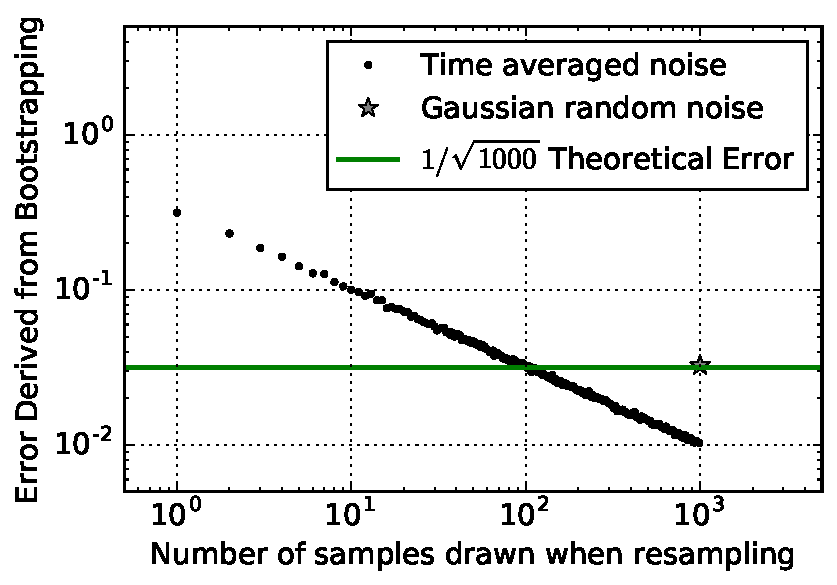
\includegraphics[trim={0cm 0cm 0cm 0cm},width=\columnwidth]{plots/toy_error1.pdf}
%	\caption{Error estimation from bootstrapping as a function of the number of elements drawn per bootstrap when 
%sampling with replacement. The star represents the standard deviation of $N_{\rm boot}=500$ bootstraps, each created by drawing $1000$ elements (with replacement) from a length $1000$ array of a Gaussian random signal. The black points correspond to time-averaged data (correlated data) which has $100$ independent samples. They illustrate how errors can be underestimated if drawing more elements than there are independent samples in the data. The estimated errors match up with the theoretical prediction only at $N=100$.}
%	\label{fig:toy_error1}
%\end{figure}

This is the precisely how errors were underestimated in PAPER-64. Because of fringe-rate filtering, which averages data in time to increase sensitivity, PAPER-64 data is correlated along the time axis. Hence, there are fewer independent samples after filtering, thus decreasing the variance of the bootstraps.

More specifically, the PAPER-64 pipeline outputs $20$ bootstraps (over baselines), each a $2$-dimensional power 
spectrum that is a function of $k$ and time. In \citetalias{ali_et_al2015}, a second round of bootstrapping occurred over the time axis, and a total of $400$ bootstraps were created in this step, each comprised of randomly selected values sampled with replacement (i.e., each of these bootstraps contained the same number of values as the number of time integrations, which, at $\sim$
$700$, greatly exceeds the approximate number of independent samples after fringe-rate filtering).
Means were then taken of the values in each bootstrap. Finally, power 
spectrum limits were computed by taking the mean and standard deviation over all the bootstraps. We emphasize again that in 
this previous analysis, the number of elements sampled per bootstrap greatly 
exceeded the number of independent LST samples, underestimating errors. A random draw of $700$ 
measurements from this dataset has many repeated values, and the variance between hundreds of these random 
samples is smaller than the true underlying variance of the data. 

Given our new understanding of the sensitivity of bootstraps to the number of elements sampled, we have removed the second 
bootstrapping step along time entirely and now simply bootstrap over the baseline axis. Power spectrum $2\sigma$ errors (computed from bootstrap variances) with and without this bootstrapping change for a fringe-rate filtered noise simulation are shown in Figure 
\ref{fig:data_errors} in black and gray, respectively. The estimates are uniformly weighted in order to disentangle the effects of bootstrapping from signal loss. As 
shown in the figure, when more elements are drawn for each bootstrap than the number of 
independent samples (by over-sampling elements along the time axis), repeated values begin to crop up and the apparent variation between bootstraps drops, resulting in limits (gray) below the predicted noise level (green). Using the revised bootstrapping method, where bootstrapping only occurs over the baseline axis, the limits (black) are shown to agree with the analytic prediction for noise. While Figure \ref{fig:data_errors} implies that errors, computed prior to our bootstrapping change (gray), are underestimated by a factor of $\sim$ $5$ in mK$^{2}$ for the noise simulation (whose creation details are outlined in the next section), in practice this factor is lower for the case of real data (a factor of $\sim$ $3$ in mK$^{2}$ instead), possibly due to the data being less correlated in time than the fringe-rate filtered noise in the simulation. 

In addition to learning how sample independence affects bootstrapped errors, we have made three additional changes to our bootstrapping procedure since \citetalias{ali_et_al2015}, summarized here:

\begin{itemize}

\item{A second change to our bootstrapping procedure is that we now bootstrap over baseline cross-products, instead of the baselines themselves. In the previous analysis, baselines were bootstrapped prior to forming cross power spectra, and using this particular ordering of operations (bootstrapping, then cross-multiplication) yields variances that have been found to disagree with predicted errors from bootstrapping using simulations. On the contrary, bootstrapping over cross power spectra ensures that we are estimating the variance of our quantity of interest (i.e., the power spectrum). This change, while fundamental in retaining the integrity of the bootstrapping method in general, alters the resulting power spectrum errors by factors of $<2$ in practice.}

\item{In \citetalias{ali_et_al2015}, individual baselines were divided into five independent groups, where no baselines were repeated in each group. Then, baselines within each group were averaged together, and the groups were cross-multiplied to form power spectra. This grouping method was used to reduce computational time, however upon closer examination it has been found that the initial grouping introduces an element of randomness into the final measurements --- more specifically, the power spectrum value fluctuates depending on how baselines are assigned into their initial groups. Our new approach removes this element of randomness at the cost of computational expense, as we now perform all baseline cross-products.}

\item{Finally, the last change from the \citetalias{ali_et_al2015} method is that our power spectrum points (previously computed as the mean of all bootstraps), are now computed as the power spectrum estimate resulting from not bootstrapping at all. More specifically, we compute one estimate without sampling, and this estimate is propagated through our signal loss computation (this estimate is $\widehat{\textbf{P}}_{x}$). The difference between taking the mean of the bootstrapped values and using the estimate from the no-bootstrapping case is small, but doing the latter ensures that we are forming results that reflect the estimate preferred by all our data.}

\end{itemize}

In summary, we have learned several lessons regarding bootstrapping and have revised our analysis procedure in order to determine error bars that correctly reflect the variance in our power spectrum estimates. Bootstrapping can be an effective and straightforward way to estimate errors of a dataset, however, bootstrapping as a means of estimating power spectrum errors from real fringe-rate filtered data requires knowledge of the number of independent samples, which is not always a trivial task. We have thus avoided this issue by removing one of our bootstrap axes, as well as updated several other details of our procedure to ensure accurate re-sampling and error estimation.

\begin{figure}
	\centering
	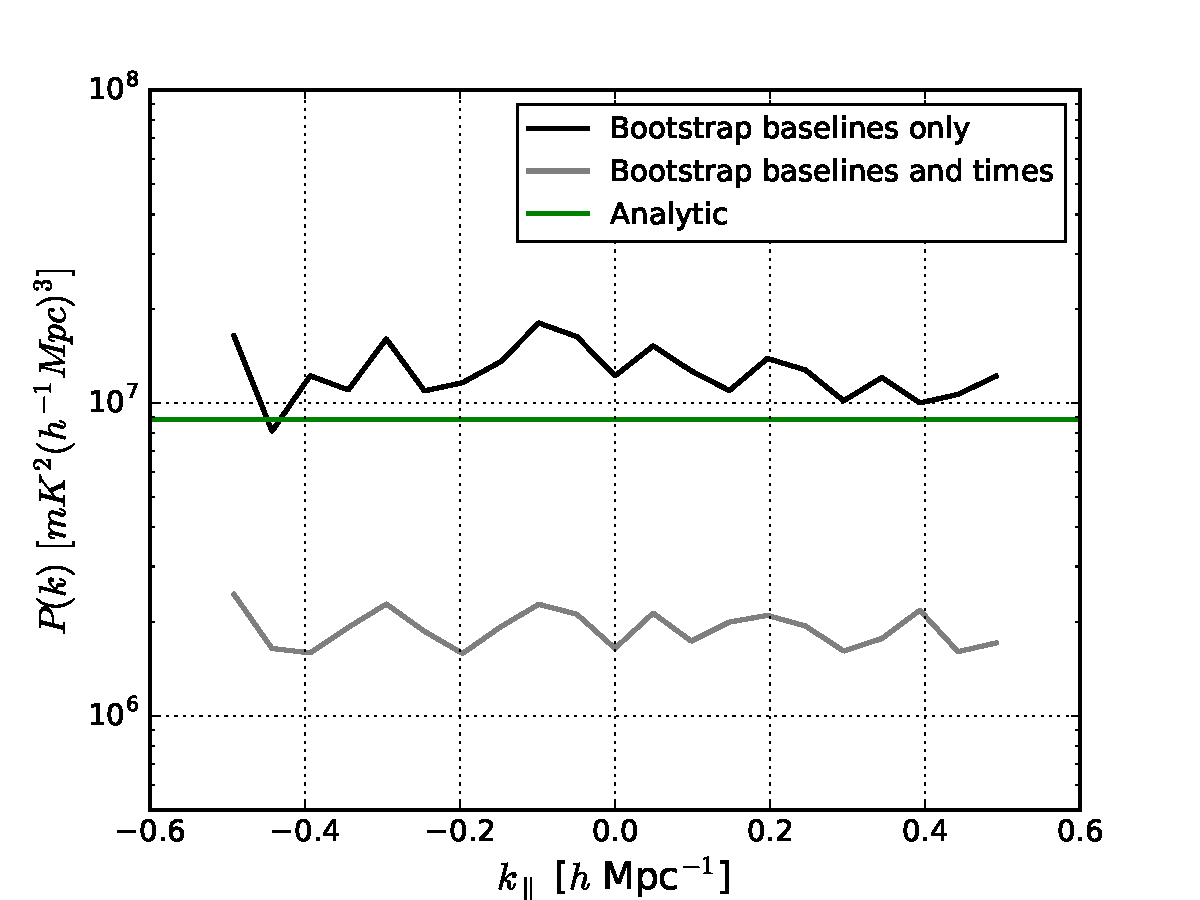
\includegraphics[trim={0.3cm 0cm 0.3cm 0.3cm},width=\columnwidth]{plots/noise_errors.pdf}
	\caption{$2\sigma$ power spectrum errors (from bootstrap variances) for a noise simulation (computed via Equation \eqref{eq:noise} using PAPER-64 observing parameters) using two different bootstrapping 
methods. The noise is fringe-rate filtered and a weighting matrix of $\textbf{I}$ (uniform-weighted) is used in order to disentangle the 
effects of bootstrapping from signal loss. The bootstrapping method used in \citetalias{ali_et_al2015} is shown in gray, where bootstrapping occurs along both the baseline and time axes. This underestimates errors by sampling more values than independent ones in the dataset (fringe-rate filtering reduces the number of independent samples along time). We use the method illustrated by the black curve in our updated analysis, where bootstrapping only occurs along the baseline axis. We find that these revised limits agree with the $2\sigma$ analytic prediction for noise (green).}
	\label{fig:data_errors}
\end{figure}

\subsection{Theoretical Error Estimation}
\label{sec:Error}

One useful way of cross-checking measured power spectrum values and errors is to compute a theoretical estimation of thermal noise based on observational parameters. Although a theoretical model often differs from true errors, it is helpful to understand the ideal case and the factors that affect its sensitivity. Upon re-analysis of PAPER-64, we have discovered that this estimate was also underestimated in previous analyses. 

To compute our theoretical noise estimate, we use an analytic sensitivity calculation. Through detailed studies using several independently generated noise simulations, what we found was that our simulations all agreed but were discrepant with the previous calculations. The analytic 
calculation is only an approximation and attempts to combine a large number of pieces of information in an approximate way; however, when re-considering some of the approximations, the differences were large enough (factors of $10$ in some cases) to warrant a 
careful investigation. What follows here is an 
accounting of the differences which have been discovered. We note that our theoretical error estimate, which is plotted as the solid green curve in many of the previous power spectrum plots in this paper, is computed with these changes accounted for.

The noise prediction $n(k)$ (\citealt{parsons_et_al2012a}; \citealt{pober_et_al2013}) for a power spectral analysis of 
interferometric 21\,cm data, in temperature-units, is:

\begin{equation}
\label{eq:sense}
N(k) = \frac{X^{2}Y \Omega_{\rm eff} T_{\rm sys}^{2}}{\sqrt{2N_{\rm lst}N_{\rm seps}}\,t_{\rm int}N_{\rm days}N_{\rm bls}N_{\rm pols}}.
\end{equation}
We will now explain each factor in Equation \eqref{eq:sense} and highlight key differences from the numbers used in \citetalias{ali_et_al2015}.

\begin{itemize}
\item $X^{2}Y$: Conversion factors from observing coordinates (angles on the sky and frequency) to cosmological coordinates (co-moving 
distances). For $z=8.4$, $X^{2}Y = 5 \times 10^{11} \, h^{-3}$ Mpc$^{3}$ str$^{-1}$ GHz$^{-1}$.
\item $\Omega_{\rm eff}$: The effective primary beam area in steradians (\citealt{parsons_et_al2010}; \citealt{pober_et_al2012}). 
The effective beam area changes with the application of a fringe-rate filter, since different parts of the beam are up-weighted and down-weighted. Using numbers from Table 1 in \citet{parsons_et_al2016}, $\Omega_{\rm eff} = 0.74^{2}/0.24$ for an optimal fringe-rate 
filter and the PAPER primary beam. 
\item $T_{\rm sys}$: The system temperature is set by:

\begin{equation}
\label{eq:sys}
T_{\rm sys} = 180\Big(\frac{\nu}{0.18}\Big)^{-2.55} + T_{\rm rcvr},
\end{equation}

where $\nu$ are frequencies in GHz (\citealt{thompson_et_al2001}). We use a receiver temperature of $144$\,K, yielding $T_{\rm sys} = 431$\,K at $150$\,MHz. 
This is lower than the $T_{\rm sys}$ of $500$\,K used in \citetalias{ali_et_al2015} because of several small miscalculation errors that were 
identified\footnote{For example, there was a missing a square root in going from a variance to a standard deviation.}.
\item $\sqrt{2}$: This factor in the denominator of the sensitivity equation comes from taking the real part of the power spectrum 
estimates after cross-multiplying two independent visibility measurements. In \citetalias{ali_et_al2015}, a factor of $2$ was mistakenly used.
\item $N_{\rm lst}$: The number of independent LST bins that go into a power spectrum estimation. The sensitivity scales as the square root 
because we integrate incoherently over time. For PAPER-64, $N_{\rm lst} = 8$.
\item $N_{\rm seps}$: The number of baseline separation types (where baselines of a unique separation type have the same orientation and length) averaged incoherently in a final power spectrum estimate. For the 
analysis in this paper, we only use one type of baseline (PAPER's 30\,m East/West baselines). However, both the updated limits in Kolopanis et al. (\textit{in prep.}) and the sensitivity prediction in Figure \ref{fig:sense_check} use three separation types ($N_{\rm seps}=3$) to match \citetalias{ali_et_al2015}.
\item $t_{\rm int}$: Length of an independent integration of the data. It is crucial to adapt this number if filtering is applied along the time axis (i.e., a 
fringe-rate filter). We compute the effective integration time of our fringe-rate filtered data by scaling the original integration time $t_{i}$
using the following:
\begin{equation}
t_{\rm int} = t_{i} \frac{\int1 \, df}{\int w^{2}(f) \,df},
\end{equation}
where $t_{i}=43$ seconds, $t_{\rm int}$ is the fringe-rate filtered integration time, $w$ is the fringe-rate profile, and the integral is 
taken over all fringe-rates. For PAPER-64, this number is $t_{\rm int} = 3857$\,s. 
\item $N_{\rm days}$: The total number of days of data analyzed. In \citetalias{ali_et_al2015}, this number was set to $135$. However, because we 
divide our data in half (to form ``even" and ``odd" datasets, or $N_{\rm datasets} = 2$), this number should reflect the number of days in each individual dataset instead of the total. Additionally, this number should be adjusted to reflect the actual number of cross-multiplications that occur between datasets (``even" with ``odd" and ``odd" with ``even", but not ``odd" with ``odd" or ``even" with ``even" in order to avoid noise biases). Finally, because our LST coverage is not $100\%$ complete (it doesn't overlap for every single day), we incorporate a root-mean-square statistic in computing a realistic value of 
$N_{\rm days}$. Our expression therefore becomes:
\begin{equation}
N_{\rm days} = \sqrt{\langle N_{i}^{2}\rangle} \sqrt{(N_{\rm datasets}^{2}-N_{\rm datasets})}
 %\frac{1}{N_{\rm days}} = \sqrt{\Big\langle\frac{1}{N_{i}^{2}} \Big\rangle_{i}},
 \end{equation}
\noindent where $i$ indexes LST and frequency channel over all datasets (\citealt{jacobs_et_al2015}). For PAPER-64, our revised estimate of $N_{\rm days}$ is $\sim47$ 
days.
\item $N_{\rm bls}$: The number of baselines contributing to the sensitivity of a power spectrum estimate. In \citetalias{ali_et_al2015}, this number was 
the total number of $30$\,m East/West baselines used in the analysis. However, using the total number of baselines ($N_{\rm bls\_total} = 51$) neglects 
the fact that the \citetalias{ali_et_al2015} analysis averages baselines into groups for computational speed-up when cross-multiplying data. Our revised estimate for the parameter is:
\begin{equation}
N_{\rm bls} = \frac{N_{\rm bls\_total}}{N_{\rm gps}}\sqrt{\frac{N_{\rm gps}^{2}-N_{\rm gps}}{2}},
\end{equation}
\noindent where, in the \citetalias{ali_et_al2015} analysis, $N_{\rm gps} = 5$. Each baseline group averages down linearly as the number of baselines 
entering the group ($N_{\rm bls\_total}/N_{\rm gps}$) and then as the square root of the number of cross-multiplied pairs \Big($\sqrt{\frac{N_{\rm gps}^{2} - 
N_{\rm gps}}{2}}$\Big). A revised \citetalias{ali_et_al2015} analysis should therefore use $N_{\rm bls} \sim 32$ instead of $51$, and this change is taken into account in Figure \ref{fig:sense_check}. However, the analysis in this paper and in Kolopanis et al. (\textit{in prep.}) no longer averages baselines into groups ($N_{\rm gps} = 1$). For the subset of data presented in this paper, $N_{\rm bls} = 10$.
\item $N_{\rm pols}$: The number of polarizations averaged together. For the case of Stokes I, $N_{\rm pols}=2$.
\end{itemize}

An additional factor of $\sqrt{2}$ is gained in sensitivity when folding together positive and negative $k$'s to form $\Delta^{2}(k)$.

Our revised sensitivity estimate for the \citetalias{ali_et_al2015} analysis of PAPER-64 is shown in Figure \ref{fig:sense_check}. 
Together, the revised parameters yield a decrease in sensitivity (higher noise floor) by a factor of $\sim7$ in mK$^{2}$. 

\begin{figure}
	\centering
	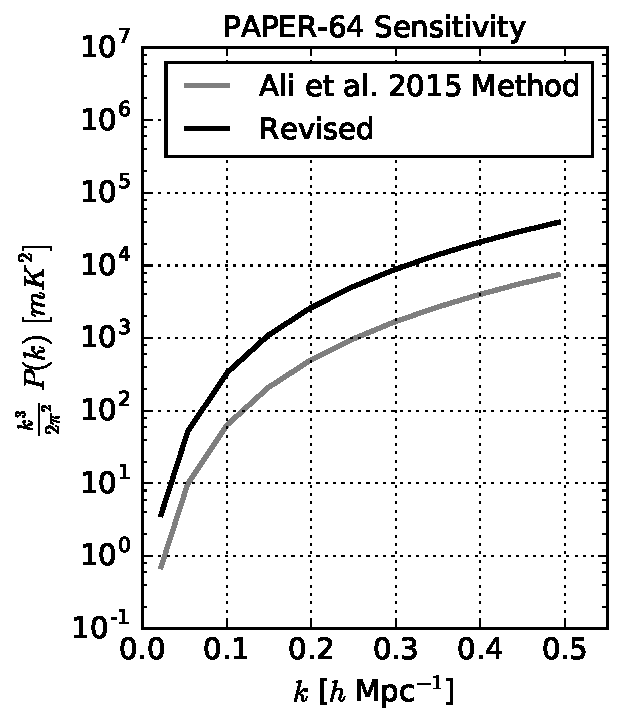
\includegraphics[width=\columnwidth]{plots/sense_check.pdf}
	\caption{An updated prediction for the thermal noise level of PAPER-64 data (black) is shown in comparison to previously 
published sensitivity limits (gray), both computed for the parameters and methods used in \citetalias{ali_et_al2015}. Major factors that contribute to the discrepancy are $
\Omega_{\rm eff}$, $N_{\rm days}$ and $N_{\rm bls}$, as in Equation \eqref{eq:sense} and described in Section \ref{sec:Error}, which when combined decreases our 
sensitivity (higher noise floor) by a factor of $\sim7$ in mK$^{2}$.}
	\label{fig:sense_check}
\end{figure}

To verify our thermal noise prediction, we form power spectra estimates using a pure noise simulation. We create Gaussian 
random noise assuming a constant $T_{\rm rcvr}$ (translated into $T_{\rm sys}$ via Equation \eqref{eq:sys}) but accounting for the true $N_{\rm days}$ as determined 
by LST sampling counts for each time and frequency in the LST-binned data. We convert $T_{\rm sys}$ into a root-mean-square variance statistic 
using:

\begin{equation}
\label{eq:noise}
T_{\rm rms} = \frac{T_{\rm sys}}{\sqrt{\Delta\nu \Delta t N_{\rm days} N_{\rm pols}}},
\end{equation}

\noindent where $\Delta\nu$ is the channel spacing, $\Delta t$ is the integration time, $N_{\rm days}$ is the number of daily counts for a 
particular time and frequency that went into our LST-binned set, and $N_{\rm pols}$ is the number of polarizations ($2$ for Stokes 
I). This temperature sets the variance of the Gaussian random noise.

Power spectrum results for the noise simulation, which uses our full power spectrum pipeline, are shown in Figure 
\ref{fig:ps_noise}. We highlight that the bootstrapped data (black and gray points, with $2\sigma$ error bars) and thermal noise prediction (solid green) show good agreement, as bootstrapping provides an accurate estimate of the noise variance. However, the limits from the full signal loss framework (weighted and unweighted in red and blue, respectively) are inflated, likely due to the additional inclusion of sample variance that comes from the EoR simulations. While the noise simulation provides an important indicator about the accuracy of our theoretical noise calculation, we note that the calculation did not take into account additional sources of error associated with earlier analysis steps (for example, \citet{trott_wayth_2017} show how calibration specifically can add errors to visibilities). Additionally, we recommend that future work investigate possible error correlations between baseline pairs and any interaction effects between signal and noise that may effect error calculations. Because of these reasons, we therefore interpret our noise prediction as the sensitivity floor for our measurements.

\begin{figure*}
	\centering
	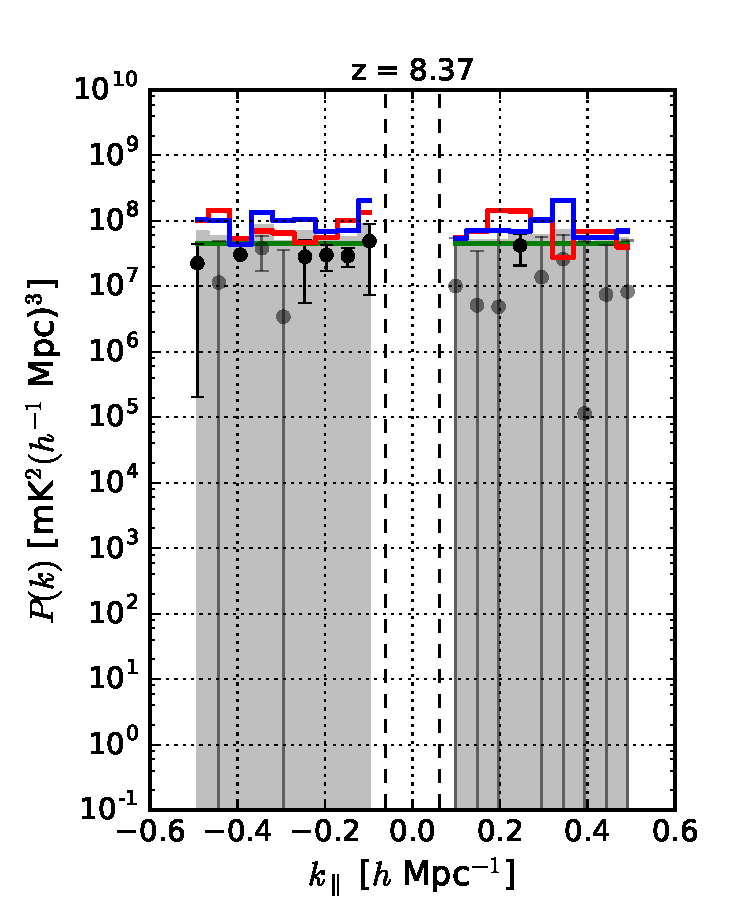
\includegraphics[width=0.4\textwidth]{plots/ps1_noise_add.pdf}
	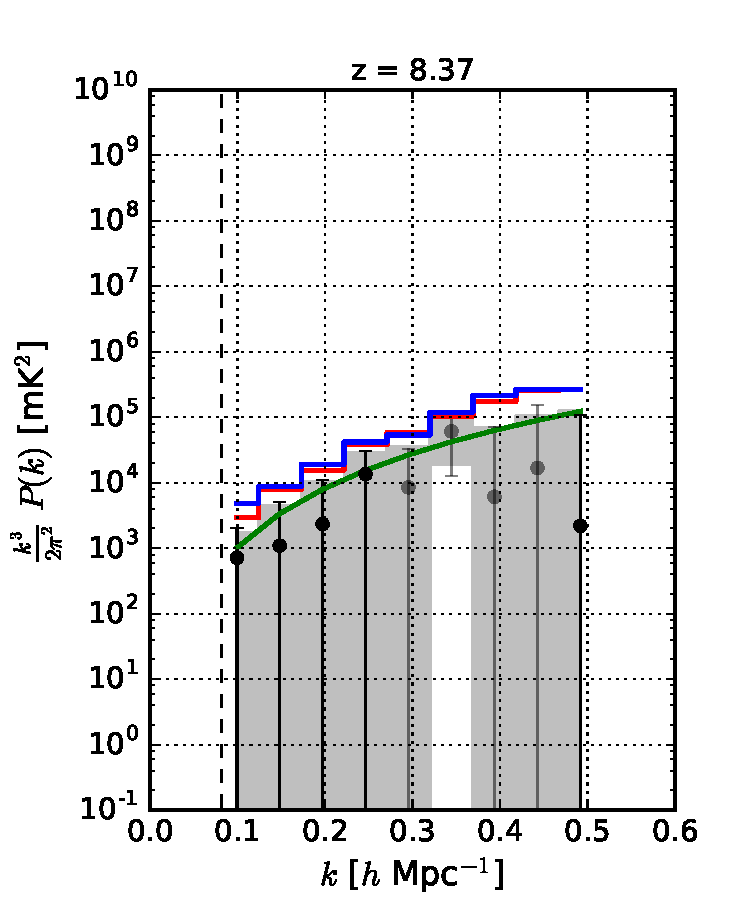
\includegraphics[width=0.4\textwidth]{plots/ps2_noise_add.pdf}
	\caption{The power spectrum for a noise simulation that mimics the noise level of a subset of PAPER-64 data, where the solid red curve is the $2\sigma$ upper limit on the EoR signal estimated from our signal injection framework using $\widehat{\textbf{C}}_{\rm eff}$. The theoretical $2\sigma$ thermal noise level prediction based on observational parameters (calculated by Equation \eqref{eq:sense}) is in green. Additionally, the power spectrum result for the uniform weighted case is shown in three different ways: power spectrum values (black and gray points as positive and negative values, respectively, with $2\sigma$ error bars from bootstrapping), the $2\sigma$ upper limit on the EoR signal using our full signal injection framework (solid blue), and the measured power spectrum values with $2\sigma$ thermal noise errors (gray shaded regions). The vertical dashed black lines signify the horizon limit for this analysis using $30$\,m baselines. We highlight that the bootstrapped data points and thermal noise prediction show good agreement, while the limits from the full injection framework (red and blue) are inflated due to the additional inclusion of sample variance that comes from the injection simulations.}
	\label{fig:ps_noise}
\end{figure*}


% CONCLUSION ---------------------------------------------------------------------------------

\section{Conclusion}
\label{sec:Con}

Although current 21\,cm published power spectrum upper limits lie several orders of magnitude above predicted EoR levels, 
ongoing analyses of deeper sensitivity datasets from PAPER, MWA, and LOFAR, as well as next generation instruments like 
HERA, are expected to continue to push towards EoR sensitivities. As the field progresses towards a detection, we have shown 
that it is crucial for future analyses to have a rigorous understanding of signal loss in an analysis pipeline and be able to accurately 
and robustly calculate both power spectrum and theoretical errors.

In particular, in this paper we have investigated the subtleties and tradeoffs of common 21\,cm power spectrum techniques on 
signal loss and error estimation, which can be summarized as follows:

\begin{itemize}
\item Substantial signal loss can result when weighting data using empirically estimated covariances due to couplings with the data realizations (Section 
\ref{sec:SiglossOverview}). Loss of the 21\,cm signal is especially significant the fewer number of independent modes that
exist in the data. Hence, there exists a trade-off between sensitivity driven 
time-averaging techniques such as fringe-rate filtering and signal loss when using empirically estimated covariances. 
\item Signal injection and recovery simulations can be used to quantify signal loss (Section \ref{sec:siglossmethod}). However, a 
signal-only simulation (i.e., comparing a uniformly weighted vs. weighted power spectrum of EoR only) can underestimate loss by 
failing to account for correlations between the data and signal which can be large and negative.
\item Errors that are estimated via bootstrapping can be underestimated if samples in the dataset are significantly correlated 
(Section \ref{sec:Boot}). However, if the number of independent samples in a dataset is well-determined, bootstrapping is a 
simple and accurate way of estimating errors.
\end{itemize}

As a consequence of our investigations, we have also used a subset of PAPER-64 data to make a new power spectrum analysis. This serves as an illustrative example of using a signal injection framework, correctly computing errors via bootstrapping, and accurately estimating thermal noise. Our revised PAPER-64 limits are presented in Kolopanis et al. (\textit{in prep.}), which supersede all previously published PAPER limits. Because of the many challenges associated with signal loss and its estimation as described in this paper, Kolopanis et al. (\textit{in prep.}) use a straightforward power spectrum estimation approach that is not lossy. However, the main reasons for a previously underestimated limit (\citealt{ali_et_al2018}) and 
ways in which our new analysis differs can still be summarized by the following:

\begin{itemize}
\item Signal loss, previously found to be $<2\%$ in \citetalias{ali_et_al2015}, was underestimated by a factor of $>$$1000$ for the case of empirically estimated inverse 
covariance weighting. Using a regularized covariance weighting method can minimize loss (Section 
\ref{sec:Weight}), however, because a regularized weighting method is not as aggressive as the former, it produces limits that are still higher than the lossy empirical inverse covariance limits. Underestimated signal loss therefore represents the bulk of our revision. 
\item Power spectrum errors, originally computed by bootstrapping, were underestimated for the data by a factor of $\sim2$ in mK due to oversampling data whose effective number of independent samples was reduced from fringe-rate filtering (Section \ref{sec:Boot}). Several other errors were also found regarding error estimation, though with smaller effects.
\item Several factors used in an analytic expression to predict the noise-level in PAPER-64 data were revised, yielding a 
decrease in predicted sensitivity level by a factor of $\sim3$ in mK (Section \ref{sec:Error}). We note that our sensitivity prediction is revised by a factor less than our overall
power spectrum result, implying that if taken at face value, the theoretical prediction for noise in \citetalias{ali_et_al2015} was too high for its data 
points.
\end{itemize}

The future of 21\,cm cosmology is exciting, as new experiments have sensitivities that expect to reach and surpass EoR levels, improved 
foreground mitigation and removal strategies are being developed, and simulations are being designed to better understand 
instruments. On the power spectrum analysis side, robust signal loss simulations and precise error calculations will play critical roles in accurate 21\,cm results. With strong foundations being established now, it is safe to say that we can expect to learn much about reionization and our early Universe in the coming years.


% ACKNOWLEDGEMENTS ---------------------------------------------------------------------------------

\section{Acknowledgements}
CC would like to acknowledge the UC Berkeley Chancellor's Fellowship and National Science Foundation Graduate Research 
Fellowship (Division of Graduate Education award 1106400). She would also like to thank Phil Bull, Bryna Hazelton, Miguel Morales, and Eric Switzer for helpful discussions. PAPER and HERA 
are supported by grants from the National Science Foundation (awards 1440343, and 1636646). ARP, DCJ, and JEA would 
also like to acknowledge NSF support (awards 1352519, 1401708, and 1455151, respectively). AL acknowledges support for this work by NASA through Hubble Fellowship grant \#HST-HF2-51363.001-A awarded by the Space Telescope Science Institute, which is operated by the Association of Universities for Research in Astronomy, Inc., for NASA, under contract NAS5-26555. SAK is supported by the University of Pennsylvania School of Arts and Sciences Dissertation Completion Fellowship. JSD acknowledges NSF AAPF
award 1701536. GB acknowledges support from the Royal Society and the Newton Fund under grant NA150184. This work is based on research supported in part by the National Research Foundation of South Africa (award 103424). We graciously thank SKA-SA for site infrastructure and observing support.
\label{sec:Ack}

% APPENDIX ---------------------------------------------------------------------------------

%\color{blue}

\begin{comment}

\appendix
\section{A toy model for inverse covariance weighting}
\label{sec:icw_appendix}

%AAAXXX

In this Appendix, we focus on the optimal quadratic estimator, Equation \eqref{eq:OQE}, and mathematically illustrate its role in estimating the power spectrum of EoR. While there exists detailed literature about quadratic estimators in general (e.g., \citealt{liu_tegmark2011}; \citealt{trott_et_al2012}; \citealt{liu_et_al2014b}; \citealt{dillon_et_al2014}), here we focus on two simple cases in order to outline one situation where the estimator successfully suppresses contamination and one where it does not. By describing these two cases, we hope to clarify and motivate the desire to use OQE while also understanding its limitations.

We specifically choose toy models where the data covariance is diagonal, as indeed we expect the EoR signal to be. We assume we have $N$ data points $\Delta_i$ which are the sum of a desired signal $\sigma_i$ and an undesired contaminant $\upsilon_i$
\begin{equation}
\Delta_i = \sigma_i + \upsilon_i
\end{equation}
with 
\begin{equation}
\langle \sigma_i \rangle = 0; \; \langle \sigma^2_i \rangle = s; \; {\rm and}~\langle \bm{\sigma \sigma}^T \rangle = s \mathbf{I}_{N \times N} \equiv \mathbf{S},
\end{equation}
where we wish to estimate $s$.  The contaminant in this first case has a similar structure (as the EoR) for its covariance, and is assumed uncorrelated with the signal
\begin{equation}
\label{eq:IdealToyModelCovariance}
\langle \upsilon_i \rangle = 0; \; 
\langle \upsilon^2_i \rangle = u; \; 
\langle \bm{\upsilon \upsilon}^T \rangle = u \mathbf{I}_{N \times N} \equiv \mathbf{U}; {\rm and}~ 
\langle \sigma_i \upsilon_j \rangle = 0.
\end{equation}
With the covariance matrix given by $\C = \mathbf{S} + \mathbf{U}$, the estimator for $s$ using only the quadratic part of Equation \eqref{eq:OQE} is
\begin{equation}
\label{eq:IdealToyModelEstimator}
\hat{s} = \frac{ \bm{\Delta^T \Delta}}{N} 
\end{equation}
and its expectation is
\begin{equation}
\langle \hat{s} \rangle = s + u.
\end{equation}
Thus, {\it when the covariance structure of the contaminant is identical to the signal} ($\PDeriv{\mathbf{S}}{s} = \PDeriv{\mathbf{U}}{u} =  \PDeriv{\C}{s}$), the information available to the quadratic portion of the estimator to distinguish between the two is degenerate, and knowledge only of $\C$ and $\PDeriv{\C}{s}$ is inadequate.  In order to obtain an unbiased estimate of $s$, one must also use knowledge of $\mathbf{U}$.  Indeed, computing the linear bias from Equation \eqref{eq:OQELinear}, one finds $b = u$.   

Now consider a case, chosen to be very similar to the toy model in \ref{sec:toymodel},  in which the data again have an additive contaminant, now given by
\begin{equation}
\Delta_i = \sigma_i + \upsilon m_i
\end{equation}
where the properties of $\sigma_i$ are as before, but now $\upsilon$ is a random variable and $m_i$ is a fixed function of $i$ with
\begin{equation}
\langle \upsilon \rangle = 0; \;
\langle \upsilon^2 \rangle = u; \; 
 \langle \bm{\upsilon \upsilon}^T \rangle = u \mathbf{m m}^T \equiv \mathbf{U}; \;
 \mathbf{m}^T \mathbf{m} = 1; \; {\rm and}~ 
\langle \sigma_i \upsilon \rangle = 0.
\end{equation}
Here $\mathbf{m}$ represents a mode which is correlated across many data points (i.e., we are assuming $\mathbf{U}$ need {\it not} be diagonal), with amplitude given by  $\upsilon$.  The normalization of $\mathbf{m}$ is a matter of convention, and can be absorbed in the variance $u$; the choice above will be convenient for understanding the limiting case $u \gg s$.

We can calculate the quadratic portion of the estimator explicitly by using the Sherman-Morrison identity to invert the covariance matrix.  Defining
\begin{equation}
\xi \equiv \frac{u/s}{1+u/s},
\end{equation} 
we have
\begin{equation}
\invC  =   \frac{1}{s} \left(\I - \xi \mathbf{m m}^T \right)
\end{equation}
and
\begin{equation}
\hat{s} = 
%\half {\F}^{-1} \left(\bm \Delta^T \invC \PDeriv{\C}{s}  \invC \bm \Delta \right) = 
\frac{ \bm \Delta^T  (\I +  (\xi^2 - 2 \xi)  \mathbf{m m}^T)  \bm \Delta}{N + \xi^2 - 2 \xi} 
\end{equation}
with expectation
\begin{equation}
\langle \hat{s} \rangle = 
s + \frac{1 - 2 \xi + \xi^2}{N + - 2 \xi + \xi^2} u. 
\end{equation}
It is worth observing immediately that there is no multiplicative bias on $s$, and that the additive bias is strictly $< u/N$.

An instructive limit is $u \gg s$, $\xi \to 1$, in which case the virtue of weighting by $\invC$ becomes clearer, as it becomes
\begin{equation}
\invC  = \frac{1}{s} \left(\I - \mathbf{m m}^T \right)
\end{equation}
where $\I - \mathbf{m m}^T$ is the projection operator, projecting out $\mathbf{m}$ from any vector it acts on, and further, the linear bias tends to 0 as $\xi \to 1$ (i.e., the projection is ``perfect'' and not ``undone'' by the Fisher matrix normalization).

This is the ideal case for the inverse covariance weighting performed in the PAPER analysis, where removal of contamination with a known covariance can be suppressed by a kind of projection of the offending modes.  But even in this case, it is worth pointing out that the estimator still has a linear bias for finite $u$.  We have also assumed that the contaminating mode $\mathbf{m}$ is known perfectly; the next appendix takes up the case where the modes are estimated from the data.

\color{black}

%\appendix
\section{A toy model for signal loss}
\label{sec:sigloss_appendix}

In this Appendix, we examine a toy model for signal loss. Our goal is to derive an analytic formula for power spectrum signal loss. While this model does not apply generally to all the scenarios presented in this paper, it provides some analytic intuition for how the coupling between data and an empirical covariance can result in signal loss.

The minimum-variance quadratic estimator $\widehat{P}^\alpha$ for the $\alpha$th bandpower of the power spectrum is given by 
\begin{equation}
\widehat{P}^\alpha = \frac{1} {2 \F^{\alpha \alpha} }\x^t \C^{-1} \Q^{\alpha} \C^{-1} \x,
\end{equation}
where
\begin{equation}
F^{\alpha \alpha} \equiv \frac{1}{2} \textrm{tr} \left( \C^{-1} \Q^\alpha \C^{-1} \Q^\alpha \right)
\end{equation}
is the $\alpha$th diagonal element of the Fisher matrix. For this section only, with no loss of generality, we assume that the data $\textbf{x}$ are real. We also assume for simplicity that $\mathbf{x}$ is the data from a single instant in time, so that it is of length $N_f$, where $N_f$ is the number of frequency channels.

In our case, we do not have \emph{a priori} knowledge of the covariance matrix. Thus, we deviate from the true minimum-variance quadratic estimator and replace $\C$ with $\Chat$, its data-derived approximation. Our estimator then becomes
\begin{equation}
\label{eq:phatloss}
\widehat{P}^\alpha_\textrm{loss} = \frac{1} {2 \widehat{\F}^{\alpha \alpha} }\x^t \Chat^{-1} \Q^{\alpha} \Chat^{-1} \x,
\end{equation}
where
\begin{equation}
\widehat{F}^{\alpha \alpha} \equiv \frac{1}{2} \textrm{tr} \left( \Chat^{-1} \Q^\alpha \Chat^{-1} \Q^\alpha \right),
\end{equation}
with the label ``loss" to foreshadow the fact that this will be an estimator with signal loss (i.e., a multiplicative bias of less than unity). We will now provide an explicit demonstration of this by modeling the estimated covariance as
\begin{equation}
\label{eq:ChatDef}
\Chat = (1-\eta) \C + \eta \x \x^t,
\end{equation}
where $\eta$ is a parameter quantifying our success at estimating the true covariance matrix. If $\eta = 0$, our covariance estimate has perfectly modeled the true covariance and $\Chat = \C$. On the other hand, if $\eta =1$, then our covariance estimate is based purely on the one realization of the covariance that is our actual data, and we would expect a high level of overfitting and signal loss.

Our strategy for computing the signal loss will be to insert Equation \eqref{eq:ChatDef} into Equation \eqref{eq:phatloss} and to express the resulting estimator $\widehat{P}^\alpha_\textrm{loss}$ in terms of $\widehat{P}^\alpha$. We begin by expressing $\Chat^{-1}$ in terms of $\C^{-1}$ using the Woodbury identity so that
\begin{equation}
\Chat^{-1} = \frac{\C^{-1}}{1-\eta} \left[ \I - \frac{\eta \x \x^t \C^{-1}}{1+ \eta (g-1)}\right],
\end{equation}
where we have defined $g \equiv \x^t \C^{-1} \x$. Inserting this into our Fisher estimate we have
\begin{equation}
\widehat{F}^{\alpha \alpha} = \frac{F^{\alpha \alpha}}{(1-\eta)^2} \left[ 1 -\frac{\eta }{1+ \eta (g-1)} \frac{h^{\alpha \alpha}}{F^{\alpha \alpha}} + \frac{1}{2} \left( \frac{\eta }{1+ \eta (g-1)} \right)^2 \frac{(h^{\alpha})^2}{F^{\alpha \alpha}}\right],
\end{equation}
where $h^\alpha \equiv \x^t \C^{-1} \Q^\alpha \C^{-1} \x $ and $h^{\alpha \alpha} \equiv \x^t \C^{-1} \Q^\alpha \C^{-1} \Q^\alpha \C^{-1}\x $. Note that $g$, $h^\alpha$, and $h^{\alpha \alpha}$ are all random variables, since they depend on $\x$. Inserting these expressions into our estimator gives
\begin{equation}
\label{eq:phatlossexpanded}
\widehat{P}^\alpha_\textrm{loss} = \frac{1}{2} \frac{h^\alpha}{F^{\alpha \alpha}} \left[ 1 - \frac{\eta g}{1+ \eta (g-1)}\right]^2  \left[ 1 -\frac{\eta }{1+ \eta (g-1)} \frac{h^{\alpha \alpha}}{F^{\alpha \alpha}} + \frac{1}{2} \left( \frac{\eta }{1+ \eta (g-1)} \right)^2 \frac{(h^\alpha)^2}{F^{\alpha \alpha}}\right]^{-1}.
\end{equation}
Both for the purposes of analytical tractability and to provide intuition, we expand this expression to leading 
order in $\eta$. This approximates the limiting case where the covariance $\Chat$ is close to the ideal and the 
lossy covariance is a small perturbation.  The result is
\begin{equation}
\widehat{P}^\alpha_\textrm{loss} \approx \frac{1}{2} \frac{h^\alpha}{F^{\alpha \alpha}} \left[ 1 - \eta \left( g - \frac{h^{\alpha \alpha}}{F^{\alpha \alpha}}\right)\right].
\end{equation}
Taking the ensemble average of both sides and noting that the true power spectrum $P^\alpha$ is equal to $\langle h^\alpha \rangle / 2 F^{\alpha \alpha}$, we obtain
\begin{equation}
\langle \widehat{P}^\alpha_\textrm{loss} \rangle \approx (1- \eta N_f) P^\alpha + 4 \eta \frac{\rm{tr} (\C^{-1} \Q^\alpha \C^{-1} \Q^\alpha \C^{-1} \Q^\alpha )}{\left[ \rm{tr} (\C^{-1} \Q^\alpha \C^{-1} \Q^\alpha  ) \right]^2} \approx (1- \eta N_f) P^\alpha,
\end{equation}
where recall that $N_f$ is the length of $\x$, or the number of frequency channels. In the last step we dropped the final term, since it scales as $\eta P^\alpha$ (without the factor of $N$) and is therefore typically small compared to the terms that have been retained.

Recalling that $P^\alpha$ is the \emph{true} power spectrum, one sees that when the covariance in the optimal quadratic estimator is naively replaced by an empirical covariance, the resulting power spectrum estimate is biased low, i.e., there is signal loss. This occurs because of couplings between $\widehat{\C}$ and $\x$, which formally means that what was originally a quadratic estimator is no longer quadratic, but contains higher-order correlations. This violates the assumptions implicit in the derivation of $F^{\alpha \alpha}$ as the normalization factor for converting unnormalized bandpowers $\frac{1}{2} \x^t \C^{-1} \Q^{\alpha} \C^{-1} \x$ into properly normalized power spectrum estimates, where the unnormalized bandpowers are assumed to be two-point (i.e., quadratic) statistics \citep{liu_tegmark2011}. The result is an improperly normalized---and thus lossy---power spectrum estimate.

\section{Derivation of the Jeffreys Prior}
\label{sec:jeffreys}

The Jeffreys prior is an objective, non-informative prior distribution for a parameter space using Bayesian probability (\citealt{jaynes1968}). For the signal injection framework outlined in Section \ref{sec:Practice}, we wish to compute the prior $p(P_{\rm in})$, or the probability density of the power spectrum of the EoR signal. 

The Jeffreys prior is defined as: 

\begin{equation}
\label{eq:jeffreys}
p(P_{\rm in}) \propto \sqrt {\Bigg\langle \Bigg(\frac{\partial \mathcal{L}}{\partial P_{\rm in}} \Bigg)^{2}\Bigg\rangle},
\end{equation}

\noindent where

\begin{equation}
\label{eq:logprob}
\mathcal{L} = \mathrm{ln} \, p(\widehat{P}_{\rm out} | P_{\rm in}),
\end{equation}

\noindent recalling that in our framework $P_{\rm in}$ is the power spectrum of the EoR signal (uniformly weighted), and $\widehat{P}_{\rm out}$ is the weighted output power spectrum of the data plus EoR.

For a single injection amplitude, our bootstrapped $\widehat{P}_{\rm out}$ values are well-approximated by a Gaussian distribution. Simplifying our notation so that $x = P_{\rm in}$ and $y = \widehat{P}_{\rm out}$:

\begin{equation}
\label{eq:prob}
p(y | x) = \frac{1}{\sigma(x) \sqrt{2\pi}} e^{-\frac{1}{2}\big(\frac{y-\bar y(x)}{\sigma}\big)^{2}},
\end{equation}

\noindent where $\sigma$ is the standard deviation of $\widehat{P}_{\rm out}$ and $\bar y$ is the mean of $\widehat{P}_{\rm out}$, and they are both functions of $P_{\rm in}$. Combining Equations \eqref{eq:jeffreys}, \eqref{eq:logprob}, and \eqref{eq:prob} the Jeffreys prior simplifies to become:

%\begin{eqnarray}
%\Big(\frac{\partial \mathcal{L}}{\partial x} \Big)^{2} &=& \frac{1}{\sigma^{2}}\Big(\frac{\partial \sigma}{\partial x}\Big)^{2} -  \Big(\frac{2(y-\bar y)}{\sigma^{3}}\Big)\frac{\partial \sigma}{\partial x}\frac{\partial \bar y}{\partial x} - \Big(\frac{2(y-\bar y)^{2}}{\sigma^{4}}\Big)\Big(\frac{\partial \sigma}{\partial x}\Big)^{2} \nonumber \\
%&+& \Big(\frac{(y-\bar y)^{2}}{\sigma^{4}}\Big)\Big(\frac{\partial \bar y}{\partial x}\Big)^{2} + \Big(\frac{2(y-\bar y)^{3}}{\sigma^{5}}\Big)\frac{\partial \sigma}{\partial x}\frac{\partial \bar y}{\partial x} + \Big(\frac{(y-\bar y)^{4}}{\sigma^{6}}\Big)\Big(\frac{\partial \sigma}{\partial x}\Big)^{2}.
%\end{eqnarray}

%Taking the expectation value then removes all terms with odd powers of $(y - \bar y)$ because those Gaussian moments evaluate to zero. Additionally, the second moment can be simplified since $\langle (y - \bar y)^{2} \rangle = \sigma^{2}$ and the fourth moment can be simplified since $\langle (y - \bar y)^{4} \rangle = 3\sigma^{4}$. Finally, after some additional simplification the Jeffreys prior becomes:

\begin{equation}
\label{eq:jeffreys_final}
p(x) \propto \sqrt{ \frac{1}{\sigma^{2}}\Big(2\Big(\frac{\partial \sigma}{\partial x}\Big)^{2} + \Big(\frac{\partial \bar y}{\partial x}\Big)^{2}\Big) }.
\end{equation}

When we simulate our full injection framework as in Section \ref{sec:Practice}, we sample 50 $P_{\rm in}$ values that range from $\sim$ $10^{5}$\,mK$^{2}$ ($h^{-1}$ Mpc)$^{3}$ to $\sim$ 10$^{11}$\,mK$^{2}$ ($h^{-1}$ Mpc)$^{3}$, and we note that the prior is set to zero outside those regions. For the injections that we do sample, we can simply fit analytic functions to the mean and standard deviations of $\widehat{P}_{\rm out}$ ($\bar y$ and $\sigma$) as functions of $P_{\rm in}$. %An example of the typical shape of these functions for the PAPER-64 analysis is shown in Figure \ref{fig:jeffreys1}, though in practice we fit solutions for every $k$-value and simulation independently.

%\begin{figure}
%	\centering
%	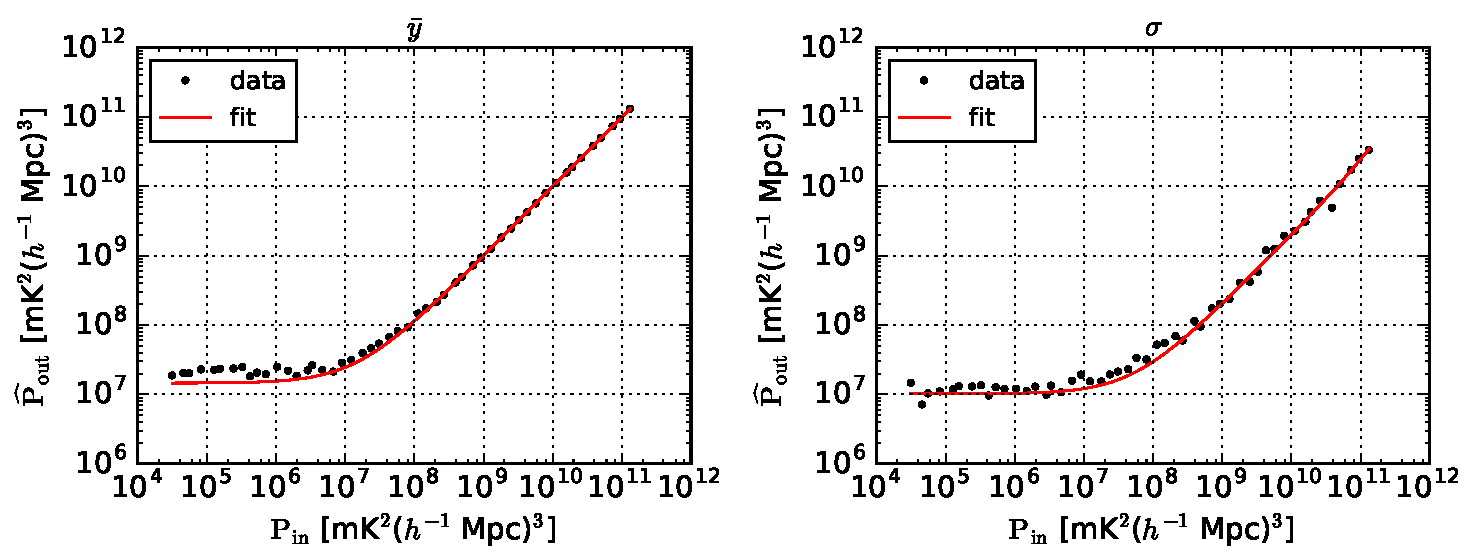
\includegraphics[width=\columnwidth]{plots/jeffrey_fits.pdf}
%	\caption{An illustrative example (for the PAPER-64 analysis using uniform weighting and $k=0.393$\,$h$ Mpc$^{-1}$) of how the mean of $P_{\rm out}$ (left) and standard deviation of $P_{\rm out}$ (right) behave as a function of $P_{\rm in}$. Polynomials are fit to each (red) to describe how $\bar y$ and $\sigma$ evolve with $x$ (injection level), respectively, for the computation of the Jeffreys prior as defined in Equation \eqref{eq:jeffreys_final}. The polynomial fits for this example are $y = (-5.1 \times 10^{-15})x^{2} + x + (1.5 \times 10^{7})$ and $y = (5.0 \times 10^{-13})x^{2} + 0.2 x + 10^{7}$ for $\bar y$ and $\sigma$, respectively.}
%	\label{fig:jeffreys1}
%\end{figure}

We show the typical shape of the Jeffreys prior used in our analysis in Figure \ref{fig:jeffreys2}, as computed by Equation \eqref{eq:jeffreys_final}. Most noticeably, it is not constant with $P_{\rm in}$, meaning a uniform prior, which is often used for simplicity, is informative in our application. Therefore, due to its objective nature we choose to use a Jeffreys prior in our analysis, multiplying our likelihood functions by Equation \eqref{eq:jeffreys_final} before computing posterior distributions.

\begin{figure}
	\centering
	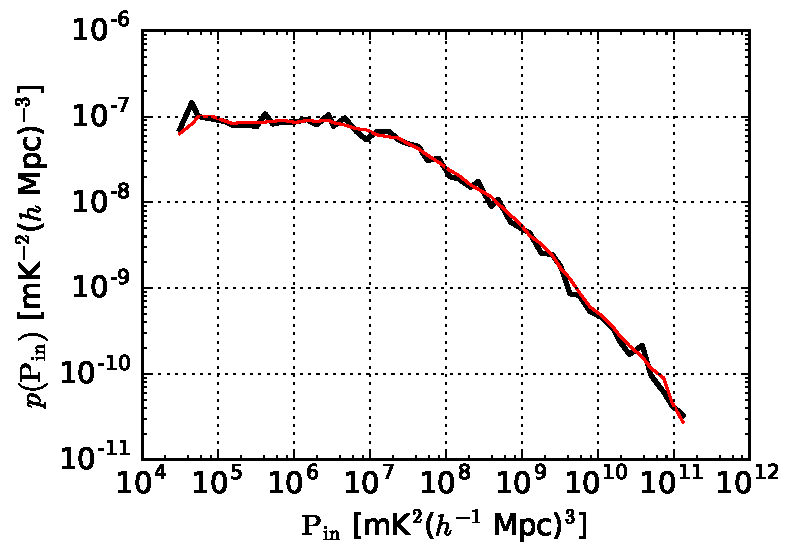
\includegraphics[width=10cm]{plots/jeffrey_prior.pdf}
	\caption{An example of the typical Jeffreys prior shape for the PAPER-64 analysis as computed by Equation \eqref{eq:jeffreys_final} (black). We smooth the prior using a sliding boxcar average over every $5$ injection levels (red). Most noticeably, the Jeffreys prior is not constant with $P_{\rm in}$, meaning a uniform prior would be an informative prior.}
	\label{fig:jeffreys2}
\end{figure}

\end{comment}

\bibliographystyle{apj}
\bibliography{refs}

\end{document}

